\documentclass[pdftex,11pt]{book}
\usepackage[pdftex]{graphicx}
\usepackage[activeacute,spanish]{babel}
\usepackage[T1]{fontenc}
\usepackage[protrusion=true,expansion=true]{microtype}
\usepackage{enumitem}
\usepackage{lmodern}
\usepackage[latin1]{inputenc}
\usepackage{geometry}
\geometry{verbose,dvips,paperwidth=5in,paperheight=8in,tmargin=.65in,bmargin=.9in, left=0.80in, right=0.65in}
\usepackage{lettrine}
\usepackage[raggedright]{titlesec}

\newcommand{\degree}{\ensuremath{^\circ}}

\setcounter{secnumdepth}{0} 
\setcounter{tocdepth}{2}

\titleformat{\section}
  {\raggedright\normalfont\scshape}{\thesection}{1em}{}
	
\titleformat{\subsection}
  {\raggedright\normalfont\slshape}{\thesection}{1em}{}	
	
\widowpenalty=10000
\clubpenalty=10000
\brokenpenalty=10000\relax

\setlist[itemize]{leftmargin=*, noitemsep}

\makeatletter
\def\@makechapterhead#1{%
  \vspace*{20\p@}%
  {\parindent \z@ \raggedright
    \Large
    \ifnum \c@secnumdepth >\m@ne
        \textsc{\Large#1}
        \par\nobreak    
    \fi
    \interlinepenalty\@M
    \vskip 110\p@
  }}
  
  \def\notesname{}%


\def\@makeschapterhead#1{%
  \vspace*{20\p@}%
  {\parindent \z@ \raggedright
    \Large
    \ifnum \c@secnumdepth >\m@ne
        \textsc{\Large#1}
        \par\nobreak    
    \fi
    \interlinepenalty\@M
    \vskip 110\p@
  }}
  
  \def\notesname{}%

\makeatletter

\usepackage{fancyhdr}
\fancyhead[LE,RO]{}
\fancyhead[CE,CO]{}
\fancyhead[RE,LO]{}
\fancyfoot[LO,RE]{}
\fancyfoot[CE,CO]{}
\fancyfoot[LE,RO]{\thepage}

\usepackage{hyperref}

\begin{document}

\renewcommand{\headrulewidth}{0pt}

\normalsize

\newpage
\thispagestyle{empty}
\mbox{}

\newpage
\thispagestyle{empty}
\mbox{}

\begin{frontmatter}
\pagestyle{empty}

\vspace*{3cm}
\begin{center}
\Large{\emph{Introducci�n a los Sistemas de Informaci�n Geogr�fica}}
\end{center}
\newpage

\null
\vfill
\scriptsize
\noindent
Introducci�n a los Sistemas de Informaci�n Geogr�fica\\
Copyright \copyright 2016 V�ctor Olaya\\

\vspace{10mm}
\noindent Versi�n revisada el \today{}\\

\vspace{6mm}
\noindent
Se concede permiso para copiar, distribuir o modificar esta obra bajo los t�rminos expresados en la licencia Creative Common Atribuci�n, la cual puede encontrarse en \url{www.creativecommons.org}. La licencia se aplica a todo el texto, as� como las im�genes creadas por el propio autor, que ser�n aquellas para las que no se especifique de modo expl�cito una distinta procedencia. Este libro puede descargarse y consultarse de forma libre en varios formatos, incluyendo formatos editables, en la direcci�n Web \url{http://victorolaya.com}.\\

\noindent
Los nombre de productos o corporaciones que aparecen en el texto pueden constituir marcas registradas y se emplean sin otro af�n que el meramente identificativo. Asimismo, la inclusi�n o no de uno de tales productos no expresa recomendaci�n alguna por parte del autor.\\

\vspace{5mm}
\noindent \rule{\textwidth}{1pt}

\newpage

\makeatletter
\newlength\drop
\newcommand*{\titleGM}{%
\thispagestyle{empty}
\begingroup% Gentle Madness
\drop = 0.1\textheight
\vspace*{\baselineskip}
\vfill
\hbox{%
\hspace*{0.1\textwidth}%
\rule{1pt}{\dimexpr\textheight-28pt\relax}%
\hspace*{0.05\textwidth}% 
\parbox[b]{0.75\textwidth}{%
\vbox{%
    \vspace{\drop}
    {\Large\textsc{V�ctor Olaya}\par}\vskip3.5\baselineskip
    {\Huge\bfseries\raggedright{Introducci�n a los Sistemas de Informaci�n Geogr�fica}\par}
    \vspace{2.5cm}
    \vspace{0.4\textheight}
}% end of vbox
}% end of parbox
}% end of hbox
\vfill
\null
\endgroup}
\makeatother
\titleGM

\cleardoublepage
\normalsize

\chapter*{Pr�logo}

Hace ahora m�s de cinco a�os que se public� la primera versi�n de \emph{Sistemas de Informaci�n Geogr�fica}, un libro libre sobre fundamentos de SIG en espa�ol, y apenas unos meses desde que apareci� la segunda. El libro ha tenido una acogida excelente, y mi intenci�n es seguir manteni�ndolo actualizado en la medida que sea posible, reflejando los avances que, a buen seguro, van a producirse en el campo de los SIG.

Existe, no obstante, un obst�culo importante para que el libro alcance a todos los p�blicos: su tama�o. Por su completitud, y por la complejidad propia de la disciplina, el libro es un volumen de m�s de 800 p�ginas cargadas de detalle. La segunda versi�n se presenta en un �nico tomo, frente a los dos en que consist�a la primera, pero a�n as� sigue quedando como una obra de consulta demasiado extensa para leerse de principio a fin. Para el lector que comienza a introducirse en el ambito de los SIG y no busca especializarse, resulta un volumen intimidante y es, no hay duda, dif�cil de abordar.

Este libro intenta ser una alternativa a la obra completa, de tal forma que resulte m�s accesible para quienes desean tener una perspectiva global de la disciplina de los SIG, sin entrar en detalles demasiado espec�ficos. Es, basicamente, una versi�n resumida de aquel, pensada con la idea de usarse no como libro de consulta, sino como libro de lectura. Adem�s de ser m�s breve, se presenta en un formato m�s adecuado para esta clase de prop�sito, con algunas modificaciones en su enfoque y con menos contenido gr�fico.

He respetado en l�neas generales la estructura de los cap�tulos, de modo que es f�cil para el lector que desee profundizar en uno de ellos encontrar este en el libro completo. Desde ese punto de vista, puede entenderse este libro como una especie de <<�ndice>> de su hermano mayor, un �ndice, no obstante, prolijo y con suficiente informaci�n como ofrecer al lector una visi�n detallada del mundo de los SIG.

Este es tambi�n, por supuesto, un libro libre, que espero que progrese de una forma din�mica gracias a la contribuci�n de sus lectores. Si encuentras cualquier error o quieres colaborar en mejorar estas p�ginas, no dudes en escribirme a \texttt{volayaf@gmail.com}.

\end{frontmatter} 
\pagestyle{empty}

\cleardoublepage
\vspace*{3cm}
\begin{center} 
{\Large\scshape Introducci�n a los Sistemas de Informaci�n Geogr�fica}
\end{center}

\begin{mainmatter}

\chapter{�What is a GIS?}

\pagestyle{fancy}

Most of the information that we use nowadays is georeferenced. That is, it is information to which a geographical position can be assigned, and it's thus information that has some ancillary information related to its location.


A \textbf{Geographical Information System} (GIS) is a tool to work with feoreferenced information. In particular a GIS is a system that allows the following operations:

\begin{itemize}
	\item \textbf{Reading, editing storing}, and, generally speaking, \textbf{managing} spatial data.
	\item \textbf{Analyzing} those data. That includes from simple queries to complex models, which can be performed using whether the \textbf{spatial component} of the data (the location of each value or element), the \textbf{thematic component} (the value or element itself), or both.
	\item Generating \textbf{documents} such as maps, reports, plots, etc.
\end{itemize}


A GIS is a step further from traditional maps. A map represents a rendering of a set of spatial data, and, while this rendering has a great importance within a GIS, is it but one of its many components. A GIS includes not only data and its rendering, but also all the operations that can be perform on it, which are part as well of the system.

A GIS is a flexible and versatile tool, and most disciplines today use GIS in one way or another. One of the main reasons for this is the integrative nature of GIS. The following ones are some of the main contexts in which GIS plays this integrative role.



\begin{itemize}
\item \textbf{GIS as a tool to integrate information}. A common link between most disciplines is that they study something which can be located. This allows to combine them and get results from a joint analysis. In this context, GIS provides the framework to which that information from different disciplines can be added and in which we can work with it. 

\item \textbf{GIS as a tool to integrate technologies}. A large part of the technologies that have appeared in the last years (and most likely of those that will appear in the near future) is based on using spatial information, and are connected to some extent to a GIS to extend their capabilities and their reach. Due to its central position in this group of technologies, GIS plays a central role in linking them and allowing them to establish a fluent comunication, center around its own functionalities.


\item \textbf{GIS as a tool to integrate technologies}. GIS functionalities cover a broad range of users, most of which would not have such a well-defined framework if it was not for GIS itself. As a consequence of that, there is  better coordination between them.

\item \textbf{GIS as a tool to integrate theoretical areas}}. We can understand GIS as the sum of two disciplines: geography and computer science. However, a more detailed analysis reveals that a GIS incorporates elements from many different scientific fields, such as those related to technology and data management (computer science, database design, digital image analysis), those that study the Earth from a physical point of view (geology, oceanography, ecology) or from a social and human one (antropology, geography, sociology), those that study human behaviour and understanding (psicology) or those that have themselves traditionally integrated knowledge from different fields, such as the already mentioned geography.

The term \textbf{geomatics}, derived from \emph{geography} e \emph{informatics}, is frequently used to refer to the array of scientific areas related to GIS.
\end{itemize}

With this, we have that a GIS is a system that integrates technology, informatics, people and geographical information, and whose main purpose is to capture, analize, store edit and visualize georeferenced data.


From a different point of view, a GIS can be considered as composed of five main elements:


\begin{itemize}
 \item \textbf{Data.} Data is needed for the rest of the components to make sense and be able to serve a given purpose. Geographical information, the core of GIS, lives in the data, and a detailed knowledge of the data that we use, its quality, its origin, its characteristics, and how to manage and store it is paramount to correctly understand GIS itself.

\item \textbf{Analysis.} Analysis is one of the main strengths of GIS, and one of the reasons why the first GIS were developed. Most GIS include analysis capabilities. They include formualtions that were already used with traditional cartography, others that existed but were not feasible to use without computers, and new approaches that were developed specifically after GIS appeared.

\item \textbf{Visualization}. All types of information can be represented graphically, which makes it easier to interpret it. In the particular case case of geographic information, visualizing it is not only a different way of working with that information, but indeed the main one, since it's the one we are more used to.

While maps are graphical entities, in a GIS we work with raw alphanumeric data. In order to have the same capabilities of a printed map, a GIS must be able to create visual representations from that data, including map-like ones.

The same cartographic principles that apply when designing a printed map are also valid when rendering geographic data within a GIS, and GIS users must be familiar with them. 

\item \textbf{Technology.} That includes both the GIS software and the hardware that runs it. Additional elements that are common when working with GIS data, such as peripherics user for data entering or for creating printed cartography, are also included in here.

\item \textbf{Organization.} This icludes the elements related to ensure a proper coordination between people, data and technology. As GIS gets more complex, managin the relations between its elements becomes more important.
\end{itemize}

In the following chapters, we will describe these elements in detail.




\pagestyle{empty}

\chapter{Historia de los SIG}


\pagestyle{fancy}

El desarrollo sufrido por los SIG desde sus or�genes hasta nuestros d�as es enorme. La popularizaci�n de las tecnolog�as y los esfuerzos de desarrollo llevados a cabo por un amplio abanico de ciencias beneficiarias de los SIG, todos han contribuido a redefinir la disciplina e incorporar elementos impensables entonces. 

Podemos situar el origen de los SIG al inicio de la d�cada de los \textbf{60}, como resultado de unos factores que convergen para dar lugar al desarrollo de estos. Estos factores son principalmente dos: la \textbf{necesidad creciente de informaci�n geogr�fica} y de una gesti�n y uso �ptimo esta, y la \textbf{aparici�n de los primeros computadores}. 

Las bases para la futura aparici�n de los SIG las encontramos algunos a�os antes de esa d�cada de los 60, con el desarrollo de nuevos enfoques en cartograf�a, tales como la \textbf{geograf�a cuantitativa}, que parecen predecir las necesidades futuras que un manejo informatizado de esta traer�. 

La primera experiencia relevante en la que se combinan geograf�a e inform�tica la encontramos en 1959, cuando Waldo Tobler define los principios de un sistema denominado MIMO (map in--map out) con la finalidad de aplicar los ordenadores al campo de la cartograf�a. En �l, establece los principios b�sicos para la creaci�n de datos geogr�ficos, su codificaci�n, an�lisis y representaci�n dentro de un sistema informatizado. 

El primer Sistema de Informaci�n Geogr�fica formalmente desarrollado aparece en Canad�. Este sistema, denominado CGIS (Canadian Geographical Information Systems), fue desarrollado a principios de los 60 por Roger Tomlinson, popularmente conocido como el <<padre del SIG>>.

A mediados de los 60, las aplicaciones SYMAP y GRID sientan respectivamente las bases de los dos principales enfoques a la hora de manejar informaci�n geogr�fica: el enfoque \textbf{raster} y el enfoque \textbf{vectorial}, Ambas alternativas ser�n explicadas con detalle m�s adelante en este libro. Los conceptos b�sicos para el an�lisis dentro del SIG r�ster los establece poco despues Dana Tomlin, desarrollando lo que se conoce como \textbf{�lgebra de mapas}.

Durante los a�os sesenta, se produce un gran desarrollo de los SIG a partir de esos elementos iniciales, y el SIG comienza a incorporarse a la comunidad cartogr�fica, dejando de ser una herramienta experimental.

La evoluci�n de los SIG desde entonces recorre sucesivas etapas, avanzando muy r�pidamente ante la influencia de numerosos factores externos. Esta evoluci�n tiene lugar en el propio SIG como disciplina, en las tecnolog�as que lo sustentan, en los datos, as� como en las t�cnicas y formulaciones.

\section{La evoluci�n de los SIG como disciplina}

Los SIG eran en origen una mera combinaci�n de elementos de cartograf�a cuantitativa, enlazados con los sistemas inform�ticos de la �poca. Se trataba de un territorio propio de cart�grafos y ge�grafos que intentaban adaptar sus conocimientos y necesidades a las tecnolog�as que por aquel entonces comenzaban a surgir. No obstante, desde aquellos or�genes los cambios han sido muy grandes, y se han incorporado al �mbito de los SIG un gran n�mero de otras disciplinas cuya aportaci�n e influencia puede ser equivalente o incluso superior a la de la cartograf�a o la geograf�a. 

Coincidiendo con la etapa inicial del desarrollo de los SIG, empieza a aparecer una preocupaci�n por el entorno que tiene consecuencias muy favorables para el desarrollo de todas las ciencias relacionadas, la gran mayor�a de las cuales son o ser�n usuarias directas de SIG. El SIG comienza a integrarse paulatinamente en las tareas de \textbf{gesti�n del medio}, como un apoyo imprescindible a la hora de analizar este.

Al principio de la d�cada de los 70, siendo ya claro que los SIG son herramientas con gran futuro, aparecen no solo los esfuerzos de desarrollo y estabilizaci�n de la disciplina, sino todos los restantes que dan entidad propia a la prometedora ciencia de la informaci�n geogr�fica con base inform�tica. Comienzan a celebrarse conferencias y simposios sobre SIG, y estos pasan a formar parte de los \emph{curricula} universitarios. En los a�os 80, se consolidan las revistas y foros especializados, que habr�n de llevar la disciplina a un p�blico m�s amplio.

En el aspecto comercial, la industria del SIG se consolida tambi�n en los a�os 70. \textbf{ESRI} (Environmental Systems Research Institute), empresa  pionera y l�der del sector hasta el d�a de hoy, se funda en 1969, y sus productos tienen gran importancia a la hora de convertir los SIG en un elemento de consumo. El primer SIG de c�digo abierto, \textbf{GRASS} (Geographic Resources Analysis Support System), aparece en 1985.

El mayor avance en la incorporaci�n de los SIG a entornos no profesionales tiene lugar en la primera d�cada del siglo XXI, con la aparici�n de servicios de cartograf�a tales como \emph{Google Maps}. La popularizaci�n de los \textbf{navegadores GPS}, que incorporan tanto elementos de representaci�n como de an�lisis propios de los SIG, son otro buen ejemplo de la proliferaci�n del SIG entre un p�blico no especializado.

\section{La evoluci�n de la tecnolog�a}

Tres son los bloques principales del desarrollo inform�tico con una influencia m�s marcada en el campo de los Sistemas de Informaci�n Geogr�fica:

\begin{itemize}
 \item \textbf{Salidas gr�ficas}. La evoluci�n de las capacidades gr�ficas, intensa desde sus inicios hasta nuestros d�as y a�n muy activa, ha sido seguida de cerca por los SIG, que progresivamente van incorporando mejoras tanto en la representaci�n en pantalla como en la generaci�n de mapas impresos.
\item \textbf{Almacenamiento y acceso de datos.} El aumento en el tama�o de los datos manejados en el SIG ha debido acompa�arse de mejoras en la capacidad de almacenamiento, as� como en la de lectura, para poder garantizar un uso fluido.
\item \textbf{Entrada de datos}. Los datos geogr�ficos utilizados en los primeros a�os de los SIG eran datos en papel que se digitalizaban y almacenaban mec�nicamente en tarjetas perforadas en un �nico proceso mec�nico. Desde esos sistemas mec�nicos de tarjetas hasta los modernos equipos, la aparici�n de \emph{scanners} de gran precisi�n y t�cnicas de digitalizaci�n autom�ticas, entre otros, ha cambiado completamente el �mbito de la entrada de datos para su uso en un SIG.
\end{itemize}

Adem�s del avance de estos factores, la evoluci�n general de los ordenadores afecta a todos los elementos de \emph{software} que se ejecutan sobre ellos. De las grandes computadoras se pasa a los ordenadores personales, y los programas tales como los SIG realizan tambi�n esa transici�n de una a otra plataforma.

La elaboraci�n y an�lisis de cartograf�a se convierte a finales de los a�os 80 en una tarea que puede ya llevarse a cabo en equipos personales (PC) de bajo coste, lejos de las grandes m�quinas y equipos dedicados de alto coste.

La evoluci�n de las plataformas no se detiene ah�. Las tendencias actuales apuntan a llevar los SIG de forma gen�rica a plataformas m�viles tales como tel�fonos o tabletas, especialmente indicadas para la toma de datos en campo. La combinaci�n de estos �ltimos con las tecnolog�as de posicionamiento global como el GPS se demuestra altamente pr�ctica en este aspecto.

La aparici�n de Internet es un hecho que ha modificado todos los aspectos de la sociedad actual, est�n relacionados o no con �mbito cient�fico. El primer uso relacionado con el SIG o la distribuci�n de cartograf�a lo encontramos en 1993, con la aparici�n de \emph{Xerox PARC}, el primer servidor de mapas. El primer atlas digital en linea, el Atlas Nacional de Canad�, se encuentra disponible desde 1994. Mas recientemente, ya en este siglo, los concepto de la Web 2.0 se adaptan al �mbito de los SIG y facilitan la aparici�n de lo que se conoce como \textbf{Web Mapping}.

\section{La evoluci�n de los datos}

Las primeras bases de datos geogr�ficas conten�an mapas escaneados y elementos digitalizados en base a estos. A partir de este punto, van apareciendo nuevas fuentes de datos cuya estructura es m�s adecuada para su tratamiento informatizado, y al tiempo que los SIG se adaptan a estas, surge una relaci�n bidireccional que resulta beneficiosa para ambos.

Un avance primordial en este sentido lo constituye el lanzamiento de los primeros \textbf{sat�lites de observaci�n terrestre}. Las t�cnicas existentes para la toma de fotograf�as a�reas, desarrolladas principalmente con fines militares durante la Primera Guerra Mundial (aunque iniciadas a mitad del siglo XIX con la toma de fotograf�as desde globos aerost�ticos), pasan a aplicarse a escala global con la aparici�n de sat�lites destinados a estos efectos. En 1980 se funda SPOT, la primera compa��a mundial en ofrecer con car�cter comercial im�genes procedentes de sat�lite para toda la superficie terrestre. 

Las tecnolog�as de posicionamiento y localizaci�n son otra fuente de datos de primer orden. En 1981, el sistema GPS\index{GPS} pasa a ser plenamente operativo, y en 2000 se ampl�a la precisi�n de este para uso civil. 

Al igual que las aplicaciones, los distintos tipos de datos geogr�ficos digitales se van asentando y popularizando, recibiendo progresivamente m�s atenci�n y medios. El Servicio Geogr�fico Estadounidense (USGS) publica en 1976 los primeros \textbf{Modelos Digitales de Elevaciones} (MDE), en respuesta a la gran importancia que este tipo de dato tiene dentro del nuevo contexto del an�lisis geogr�fico. En el a�o 2000 se publican los datos de la \emph{Shuttle Radar Topographic Mission}\index{SRTM}\index{Shuttle Radar Topographic Mission} (SRTM), con informaci�n altitudinal de un 80\% de la superficie terrestre a una resoluci�n de un segundo de arco (aproximadamente, 30 metros).

La aparici�n de nuevas t�cnicas tales como el LiDAR abre nuevos caminos en cuanto a la precisi�n que puede obtenerse en la caracterizaci�n del terreno, posibilitando nuevos usos y an�lisis antes no planteados.

La evoluci�n de los datos no es solo una evoluci�n t�cnica, sino tambi�n de car�cter social y organizativo. Se empieza a entender que resulta necesario formular estrategias adecuadas para la gesti�n de los datos espaciales, y se desarrollan las  denominadas \textbf{Infraestructuras de Datos Espaciales} (IDE). El ejemplo m�s destacado de estas es la IDE Nacional de los Estados Unidos (NSDI), de 1994. En Europa, la directiva INSPIRE, de 2007, pretende la creaci�n de una infraestructura similar.

Muchos de estos desarrollos y actividades se adhieren a las especificaciones establecidas por el \emph{Open GIS Consortium}\index{Open GIS Consortium}\index{OGC} (OGC), un consorcio internacional fundado en 1994 para \textbf{homogeneizar} el empleo y difusi�n de los datos geogr�ficos.

\section{La evoluci�n de las t�cnicas y formulaciones}

Una vez que se implementan los primeros SIG y se suplen las necesidades de an�lisis y gesti�n de datos espaciales que motivaron su aparici�n, comienza el proceso de desarrollar nuevas t�cnicas y planteamientos que permiten ir m�s all� en dicho an�lisis. 

Los antecedentes del an�lisis espacial son relativamente recientes. En 1854 John Snow realiz� la que puede considerarse como una de las primeras experiencias cartogr�ficas anal�ticas, al utilizar mapas de puntos para efectuar sus deducciones y localizar en Inglaterra la fuente de un brote de c�lera. 

En su libro \emph{Design with Nature} (1969), Ian McHarg define los elementos b�sicos de la \textbf{superposici�n y combinaci�n de mapas}, que, como veremos m�s adelante, son los que se aplican tanto en el an�lisis como en la visualizaci�n de las distintas \emph{capas} de datos geogr�ficos en un SIG.

Un desarrollo especialmente relevante es el experimentado por el \textbf{an�lisis del relieve}, una disciplina que con la aparici�n de los SIG sufre un salto cualitativo muy importante. La orograf�a cl�sica, con un enfoque tradicionalmente sustentado en la geolog�a y el an�lisis geomorfol�gico, va dando lugar a una ciencia cada vez m�s cuantitativa centrada en el an�lisis morfom�trico del relieve.

Junto con la componente anal�tica, otros elementos de la pr�ctica cartogr�fica evolucionan de forma similar. En 1819, Pierre Charles Dupin crea el primer \textbf{mapa de coropletas}. Con la llegada de los SIG, este tipo de mapas se convertir�n en una forma de representaci�n muy popular.

El avance en el desarrollo de las aplicaciones de dise�o asistido por ordenador (CAD), y en general de las representaciones gr�ficas por ordenador, impuls� igualmente la aparici�n y evoluci�n posterior de una nueva disciplina: la geometr�a computacional. Sobre esta se fundamenta el an�lisis vectorial dentro de un SIG, y tambi�n parte de los mecanismos que este usa para la representaci�n gr�fica de elementos.

\pagestyle{empty}

\chapter{Fundamentos geod�sicos y cartogr�ficos}

Puesto que los SIG heredan conceptos utilizados anteriormente enla elaboraci�n de mapas, es necesario conocer estos para hacer buen uso de las herramientas que un SIG ofrece. En este sentido, resultan fundamentales los elementos de la geodes�a y la cartograf�a, sin los cuales no es posible entender el contexto de un SIG.

\section{Conceptos geod�sicos b�sicos}
\pagestyle{fancy}

La caracter�stica principal de la informaci�n georreferenciada es que tiene una \textbf{localizaci�n en el espacio}, particularmente en el espacio terrestre. Esta localizaci�n se ha de dar por medio de unas \textbf{coordenadas} que la definan de forma adecuada, lo cual implica la necesidad de establecer un sistema en base al cual expresar dichas coordenadas. 

La \textbf{geodesia} es la ciencia encargada de proveer el marco te�rico en el que fundamentar lo anterior, y su objeto de estudio es \textbf{la forma de la Tierra}. La geodesia, en sus diversas ramas, proporciona m�todos y conceptos que permiten la utilizaci�n rigurosa de coordenadas.

La necesidad del estudio geod�sico surge por el hecho de que la Tierra no es plana, y cuando el territorio que pretendemos estudiar es lo suficientemente extenso, la curvatura de la Tierra no puede ser ignorada. Este es el caso que vamos a encontrar cuando trabajemos con un SIG, y es por ello que los SIG implementan los elementos necesarios para poder efectuar un manejo de la informaci�n geogr�fica riguroso y acorde con los conceptos de la geodesia.

Uno de los objetivos principales de la geodesia es establecer un sistema de referencia y definir un conjunto de puntos (conocidos como \textbf{v�rtices geod�sicos}) cuyas coordenadas en dicho sistema sean conocidas con una precisi�n elevada. Posteriormente, y en base a esos puntos, los cuales forman una \textbf{red geod�sica}, se pueden calcular las coordenadas de cualquier punto en el sistema de referencia definido.

\subsection{Superficies de referencia}

Dos conceptos b�sicos para esta tarea: el  \textbf{elipsoide de referencia} y el \textbf{geoide}.

La Tierra tiene forma esf�rica, aunque no es una esfera perfecta, sino que est� achatada, constituyendo lo que se conoce como \textbf{elipsoide}. Sobre un elipsoide, el radio de la Tierra ya no es constante, y depende del emplazamiento. Asimilar la Tierra a un elipsoide es m�s preciso que suponer la Tierra con una forma perfectamente esf�rica, y es necesario a la hora de elaborar cartograf�a de zonas no muy extensas.

Una vez que se dispone de una expresi�n te�rica para la forma de la Tierra, el siguiente paso es la determinaci�n de los par�metros que definen esta. En el caso de utilizar la esfera, hay que calcular su radio. En el caso de asumir el elipsoide como forma de referencia, deben determinarse las medidas de los semiejes menor y mayor. 

Por razones hist�ricas, existen numerosos elipsoides, derivados del trabajo de los geodestas en diferentes �pocas y lugares. Los primeros elipsoides generales, que permiten ser usados en toda la superficie terrestre, aparecen hace aproximadamente un siglo, con objeto de disponer de una referencia internacional que facilite el uso de cartograf�a en las distintas zonas del planeta. El \textbf{elipsoide WGS--84} es uno de los m�s empleados en la actualidad, ya que es el utilizado por el sistema GPS.

El geoide\index{Geoide} es la otra superficie de referencia, definida como la superficie tridimensional en cuyos puntos la atracci�n gravitatoria es constante. Se trata de una superficie equipotencial que resulta de suponer los oc�anos en reposo y a un nivel medio y prolongar estos por debajo de la superficie terrestre. 

Al igual que en el caso de los elipsoides, existen diversos geoides de referencia, y estos no son constantes en el tiempo sino que evolucionan para adaptarse a las modificaciones que tienen lugar sobre la superficie terrestre.

La figura \ref{Fig:Tres_superficies} muestra una comparaci�n esquem�tica entre las tres superficies: superficie real de la Tierra, geoide y elipsoide.

\begin{figure}
\centering
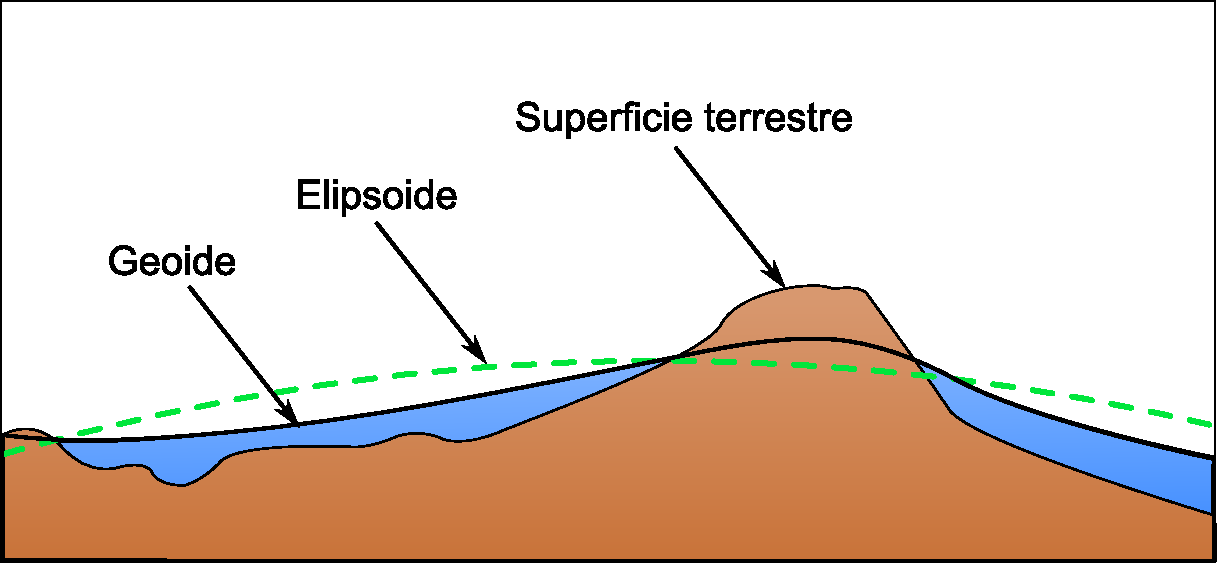
\includegraphics[width=.7\columnwidth]{Fundamentos_cartograficos/Tres_superficies.pdf}
\caption{\small Tres superficies fundamentales: superficie real de la Tierra, geoide y elipsoide (Adaptado de Wikipedia).}
\label{Fig:Tres_superficies} 
\end{figure}

En un elipsoide \textbf{general}, tanto la posici�n de su centro de gravedad como de su plano ecuatorial coinciden con los terrestres. Por el contrario, cuando el elipsoide es \textbf{local}, estas propiedades no han de cumplirse necesariamente, y el elipsoide a solas resulta insuficiente, ya que carecemos de informaci�n sobre su posicionamiento con respecto a la superficie terrestre. 

Surge as� el concepto de \textbf{datum}, que es el conjunto formado por una superficie de referencia (el elipsoide) y un punto en el que <<enlazar>> este al geoide. Este punto se denomina \textbf{punto fundamental}, y en �l el elipsoide es tangente al geoide. La vertical al geoide y al elipsoide son id�nticas en el punto fundamental. 

Para un mismo elipsoide pueden utilizarse distintos puntos fundamentales, que dar�n lugar a distintos datum y a distintas coordenadas para un mismo punto.

\subsection{Sistemas de coordenadas}

Una vez hemos definido un modelo para definir la forma de la Tierra, podemos establecer un sistema de codificar cada una de las posiciones sobre su superficie y asignar a estas las correspondientes coordenadas. Para ello, encontramos dos opciones: utilizar los elementos de la \textbf{geometr�a esf�rica} y con estos definir el sistema de referencia, o utilizar la \textbf{geometr�a plana}, para lo cual ser� necesario un mecanismo de \textbf{proyecci�n} de coordenadas que permita situar los elementos de la superficie del elipsoide sobre una superficie plana.

El sistema de \textbf{coordenadas geogr�ficas} es un sistema de coordenadas esf�ricas mediante el cual un punto se localiza con dos valores angulares: \textbf{latitud} y \textbf{longitud}. Las lineas de igual latitud o longitud se denominan \textbf{paralelos} y \textbf{meridianos} respectivamente.

Las coordenadas geogr�ficas resultan de gran utilidad, especialmente cuando se trabaja con grandes regiones. No obstante, no se trata de un sistema cartesiano, y tareas como la medici�n de �reas o distancias es mucho m�s complicada. Para poder crear cartograf�a y simplificar gran n�mero de operaciones posteriores, necesitamos coordenadas cartesianas. El proceso de asignar una coordenada plana a cada punto de la superficie de la Tierra (que no es plana) se conoce como \textbf{proyecci�n cartogr�fica}.

La superficie de la esfera no es \textbf{desarrollable}, es decir, no puede convertirse en un plano. Por ello, es necesario disponer de una metodolog�a para pasar puntos desde la superficie curva al plano, tal y como el que se muestra en la figura \ref{Fig:Proyeccion}.

\begin{figure}
\centering
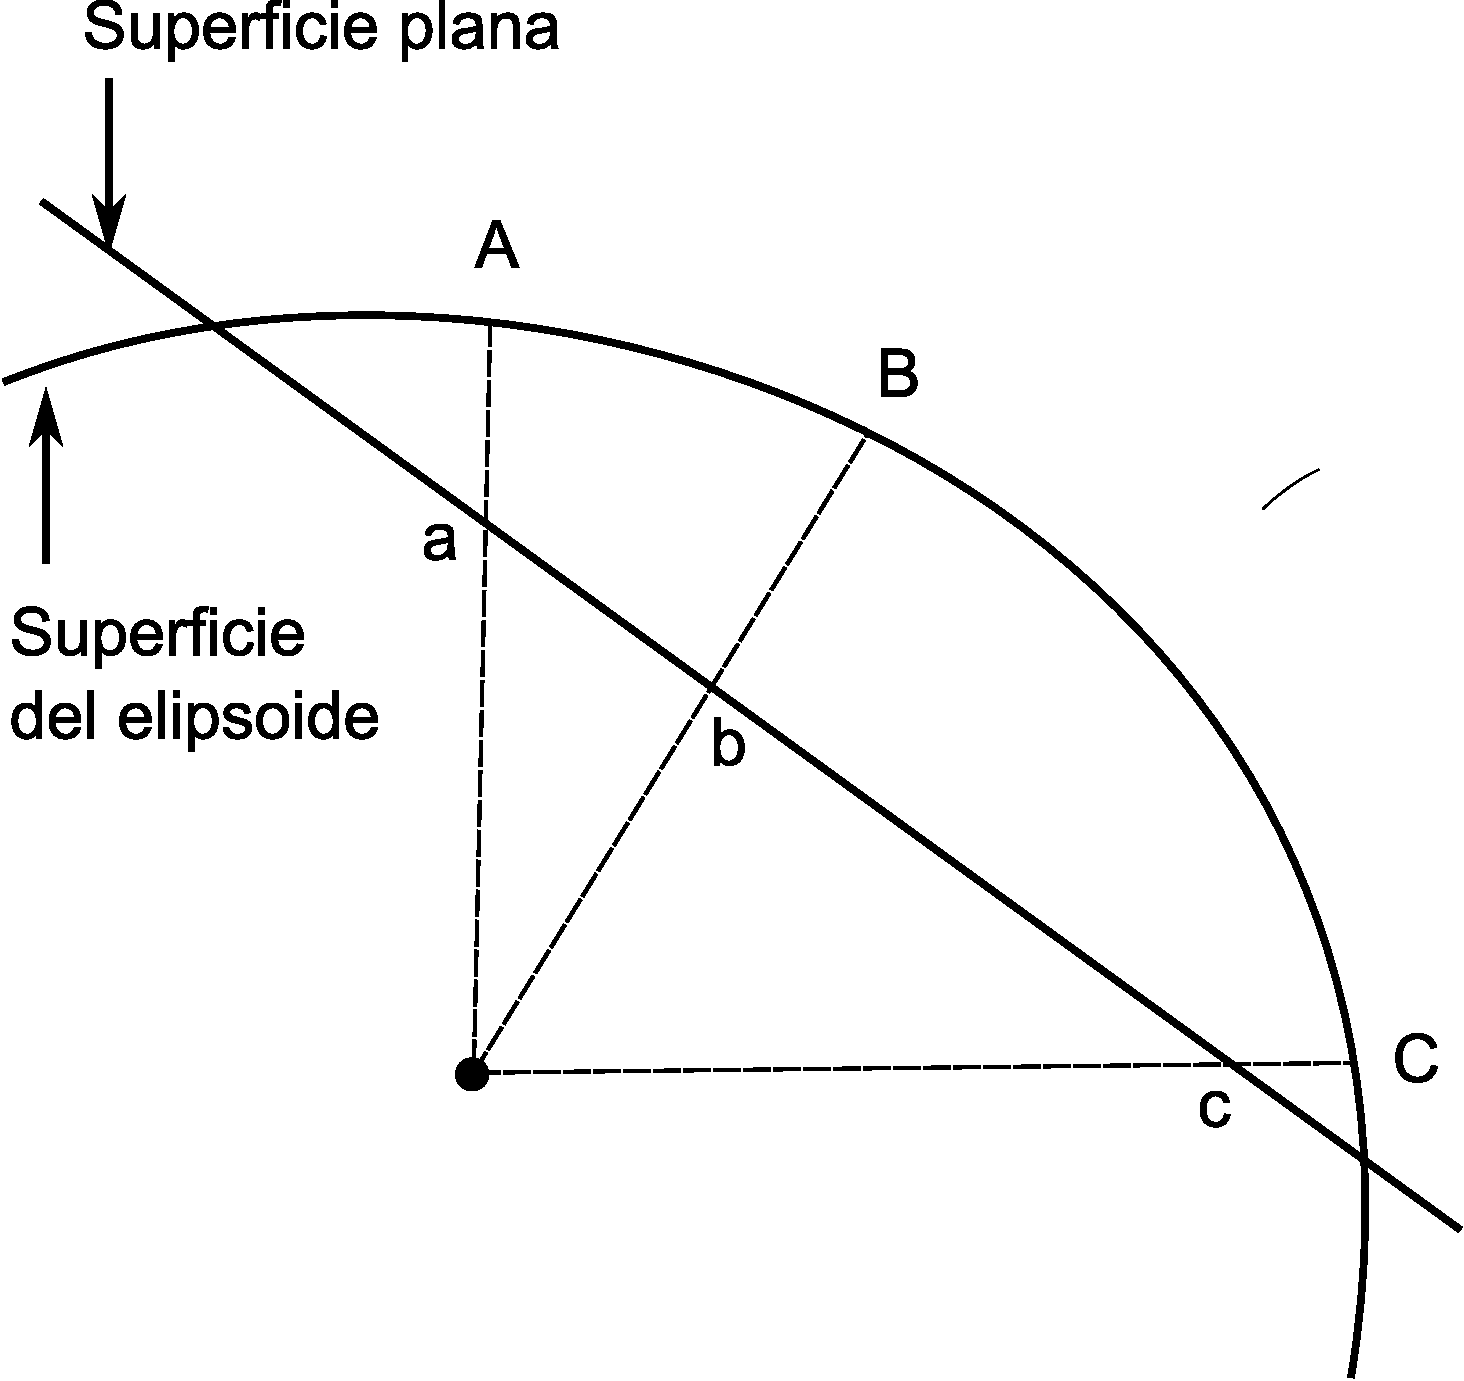
\includegraphics[width=.5\columnwidth]{Fundamentos_cartograficos/Proyeccion.pdf}
\caption{\small Esquema del concepto de proyecci�n. A los puntos $A, B$ y $C$ sobre la superficie del elipsoide se les asocian equivalentes $a, b$ y $c$ sobre un plano.}
\label{Fig:Proyeccion} 
\end{figure}


En el caso de la figura, los puntos se proyectan directamente sobre un plano. Otra opci�n es proyectarlos sobre una superficie tridimensional que, al contrario que la esfera, sea desarrollable. Las m�s habituales son el cilindro y el cono, que dan lugar a las \textbf{proyecciones c�nicas} y \textbf{cil�ndricas}.

Puede apreciarse en la figura que se producen distorsiones al realizar la proyecci�n. Por ejemplo, la distancia entre los puntos $A$ y $B$ no es igual a la existente entre los puntos $a$ y $b$. Con independencia de las caracter�sticas propias de la proyecci�n, siempre existen distorsiones, por ser la de la esfera una superficie no desarrollable. Estas distorsiones se conocen como \textbf{anamorfosis} . 


Seg�n las propiedades m�tricas que se conserven, las proyecciones pueden ser \textbf{equi�rea} (mantienen una escala constante), \textbf{conformes} (mantienen los �ngulos y la forma de los objetos) o \textbf{equidistantes} (mantienen las distancias).

La elecci�n de una u otra proyecci�n es funci�n de las \textbf{necesidades concretas} de cada caso de uso. 

En la actualidad, una de las proyecciones m�s extendidas en todos los �mbitos es la \textbf{proyecci�n universal transversa de Mercator}, la cual da lugar al \textbf{sistema de coordenadas UTM}. Este sistema no es simplemente una proyecci�n, sino un sistema completo para cartografiar la practica totalidad de la Tierra. Para ello, esta se divide en una serie de zonas rectangulares mediante una cuadricula y se aplica una proyecci�n y unos par�metros geod�sicos concretos a cada una de dichas zonas. En su forma actual, emplea un �nico elipsoide (WGS--84).

Con el sistema UTM, las coordenadas de un punto no se expresan como coordenadas terrestres absolutas, sino mediante \textbf{la zona correspondiente y las coordenadas relativas} a la zona UTM en la que nos encontremos.

La cuadricula UTM tiene un total de 60 \textbf{husos} numerados entre 1 y 60, cada uno de los cuales abarca una amplitud de 6\degree de longitud. El huso 1 se sit�a entre los 180\degree y 174\degree O, y la numeraci�n avanza hacia el Este. 

En latitud, cada huso se divide en 20 zonas, que van desde los 80\degree S hasta los 84\degree N. Estas se codifican con letras desde la C a la X, no utiliz�ndose las letras I y O por su similitud con los d�gitos 1 y 0. Cada zona abarca 8 grados de longitud, excepto la X que se prolonga unos 4 grados adicionales. 

Una zona UTM se localiza, por tanto, \textbf{con un n�mero y una letra}, y es en funci�n de la zona como posteriormente se dan las coordenadas que localizan un punto. Estas coordenadas se expresan en metros y expresan la distancia entre el punto y el origen de la zona UTM en concreto. El origen de la zona se sit�a en el punto de corte entre el meridiano central de la zona y el ecuador. 

Para evitar la aparici�n de n�meros negativos, se considera que el origen no tiene una coordenada X de 0 metros, sino de 500000, y una coordenada Y de 10000000 metros, lo cual hace que todas las coordenadas referidas a �l sean positivas.

\subsection{Transformaci�n y conversi�n de coordenadas}

Una situaci�n muy habitual en el trabajo con un SIG es disponer de cartograf�a en \textbf{varios sistemas de coordenadas}, o bien en un mismo sistema pero con par�metros diferentes (por ejemplo, diferente datum). Para poder emplear toda esa cartograf�a de forma conjunta, resulta necesario trabajar en un sistema �nico y bien definido, lo cual hace necesario convertir al menos una parte de ella. Cuando el datum es distinto en los sistemas de origen y destino, la \textbf{conversi�n de coordenadas} se conoce como \textbf{transformaci�n de coordenadas}.

Las operaciones de transformaci�n y conversi�n aparecen en los SIG como funcionalidades que permiten modificar los datos geogr�ficos, reemplazando sus coordenadas por coordenadas en otro sistema de coordenadas. Igualmente, aparecen como funcionalidades de representaci�n, permitiendo la conversi�n \textbf{al vuelo}, es decir, en tiempo real. En este caso, un dato en un sistema de coordenadas se puede representar en cualquier otro sin necesidad de una conversi�n previa, con lo que puede usarse conjuntamente con datos en un sistema de coordenadas distinto.

Para facilitar el uso de sistemas de referencia, existen proyectos de codificaci�n de estos, de forma que cada sistema existente puede identificarse de forma sencilla mediante un c�digo. El m�s extendido de estos es el sistema de codificaci�n \textbf{EPSG}.

\section{Conceptos cartogr�ficos b�sicos}

De entre los conceptos fundamentales de la cartograf�a que todo usuario de SIG ha de conocer, destaca el de \textbf{escala}. La escala  es la \textbf{relaci�n de tama�o} existente entre el mapa que se obtiene al desarrollar nuestra superficie de proyecci�n (de tama�o acorde con el objeto proyectado, esto es la Tierra) y el que finalmente manejamos, de tama�o m�s reducido. Conociendo esta relaci�n podemos conocer las verdaderas magnitudes de los elementos que vemos en el mapa, ya que podemos convertir las medidas hechas sobre el mapa en medidas reales. Es importante recordar que esas medidas no son tan <<reales>>, puesto que la propia proyecci�n las ha distorsionado ---lo cual no debe olvidarse---, pero s� que son medidas en la escala original del objeto cartografiado.

La escala se expresa habitualmente como un denominador que relaciona una distancia medida en un mapa y la distancia que esta medida representa en la realidad. Por ejemplo, una escala 1:50000 quiere decir que 1 cent�metro en un mapa equivale a 50000 cent�metros en la realidad, es decir a 500 metros. Este valor se conoce como \textbf{escala num�rica}.

Independientemente del tipo de proyecci�n, la escala es completamente cierta �nicamente en determinadas partes del mapa. En otros puntos de este, la escala var�a. La relaci�n entre la escala en esos puntos y la escala num�rica se conoce como \textbf{factor de escala}. 

Aunque tradicionalmente se entiende la escala como un concepto asociado a la representaci�n, los datos geogr�ficos tienen una escala inherente que no es funci�n de dicha representaci�n, sino del detalle con que han sido tomados. En este sentido es m�s conveniente entender la escala como un elemento relacionado con la \textbf{resoluci�n} de los datos, es decir, con el \textbf{tama�o m�nimo cartografiado}. Esta concepci�n no es en absoluto propia de los SIG, ya que deriva de las representaciones cl�sicas y los mapas impresos. Se sabe que el tama�o m�nimo que el ojo humano es capaz de diferenciar es del orden de 0,2 mm. Aplicando a este valor la escala a la que queremos crear un mapa, tendremos la m�nima distancia sobre el terreno que debe medirse. 

Es importante ser consciente de la limitaci�n que la escala considerada a la hora de la toma de datos (conocida como \textbf{escala operacional}) impone, especialmente en el contexto de un SIG. En un SIG, podemos aumentar el tama�o en pantalla de una cierta informaci�n geogr�fica, variando la escala de representaci�n (tambi�n conocida como \textbf{escala cartogr�fica}), pero ello no modifica la escala operacional. Por mucho que ampliemos no vamos a ver m�s detalles, ya que para ello ser�a necesario tomar m�s datos. 

Un tipo de datos particulares con los que se trabaja en un SIG, los datos \emph{r�ster}, tienen a su vez un par�metro de resoluci�n (el \textbf{tama�o de celda}) ligado a la escala.

Relacionado con el concepto de escala encontramos la denominada \textbf{generalizaci�n cartogr�fica}. Generalizar implicar expresar alguna idea o informaci�n de forma m�s resumida, de tal modo que esta sea comprensible y pueda aprovecharse de la mejor manera posible. La generalizaci�n es necesaria en un SIG para representar datos a una escala menor que su escala operacional, ya que a las limitaciones de la visi�n humana han de sumarse las limitaciones de resoluci�n que los dispositivos presentan. Por ejemplo, no tiene sentido representar el callejero de una ciudad a una escala peque�a como la que se utilizar�a para representar un mapa mundial, ya que cada peque�o punto de la pantalla contendr�a un gran n�mero de calles. Adem�s de obtener un resultado inservible, se consumir�an recursos en efectuar todos los c�lculos necesarios para producir esa representaci�n.

\begin{figure}[!hbt]
\centering
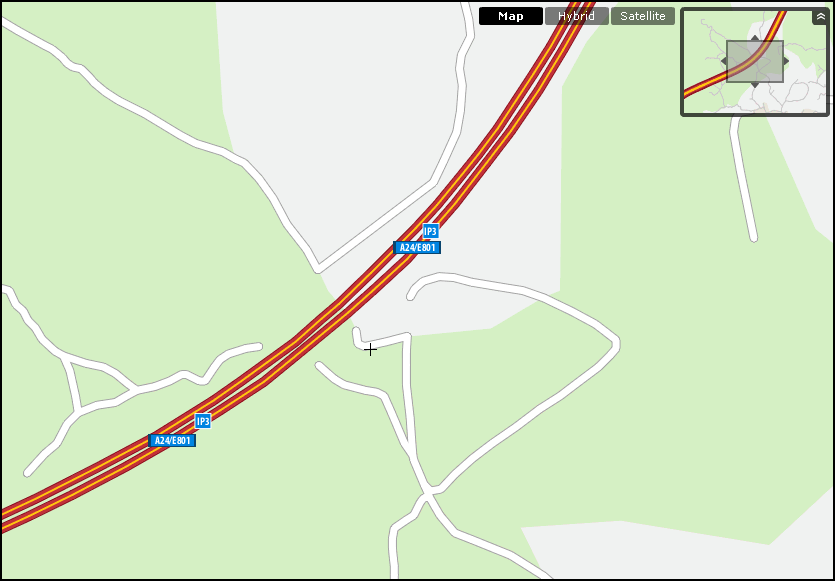
\includegraphics[width=.75\columnwidth]{Fundamentos_cartograficos/Generalizacion_agregacion.png}
\caption{\small Un ejemplo de generalizaci�n por agregaci�n. Dos carreteras pr�cticamente paralelas y unidas se representan como dos elementos en el mapa, pero en el localizador de la parte superior izquierda, a escala de menor detalle, se generalizan como una �nica (Tomado de Yahoo Maps).}
\label{Fig:Generalizacion_agregacion} 
\end{figure}


En ocasiones, el proceso de generalizaci�n es necesario por razones distintas a las anteriores, y requiere operaciones tambi�n distintas. Por ejemplo, podemos crear un mapa del mundo que contenga v�as de comunicaci�n, pero no todas, sino solo las principales autopistas de cada pa�s. En este caso, no vamos a encontrar problemas con distintas carreteras que se solapan en la representaci�n, ni tampoco un volumen excesivo de datos, pero debemos igualmente <<adaptar>> la representaci�n a la escala, es decir, efectuar alg�n tipo de generalizaci�n. En este caso, se representar�an las carreteras con un ancho mayor del real, ya que, de otro modo, no ser�an apenas visibles si las representamos con su ancho correspondiente.

La generalizaci�n, por tanto, es un proceso que tiene como objetivo la producci�n de una \textbf{imagen cartogr�fica legible y expresiva}, reduciendo el contenido del mapa a aquello que sea posible y necesario representar. Para ello, se enfatiza lo que resulta de importancia y se suprime lo que carece de ella. 

Existen diversas operaciones que se emplean en el proceso de generalizaci�n. Algunas de las m�s relevantes son las \textbf{simplificaci�n} (representar un elemento menos complejo), la \textbf{agregaci�n} (representar varios elementos como uno solo ---Figura \ref{Fig:Generalizacion_agregacion}---), la \textbf{exageraci�n} (representar elementos con mayor tama�o del que les corresponde) y el \textbf{desplazamiento} (representar en una posici�n modificada, para garantizar la legibilidad). 


\begin{figure}[!hbt]
\centering
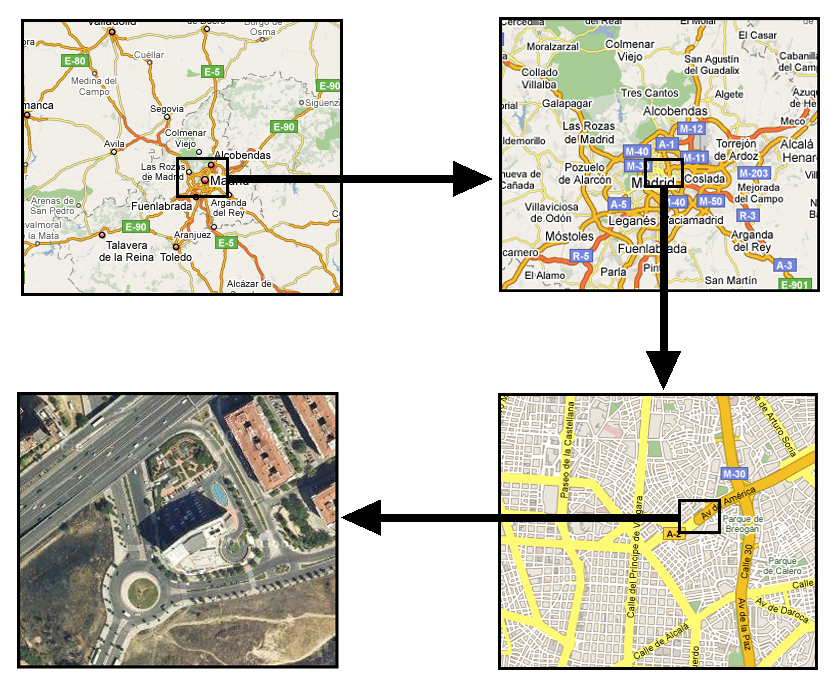
\includegraphics[width=\textwidth]{Fundamentos_cartograficos/SIG_multi_escala.png}
\caption{\small En un SIG es habitual manejar informaci�n a diferentes escalas. En funci�n de la escala de representaci�n, la informaci�n visualizada ser� una u otra.}
\label{Fig:SIG_multi_escala} 
\end{figure}


En un SIG, la generalizaci�n puede incorporarse como parte de los propios mecanismos de representaci�n, aplic�ndose las transformaci�n correspondientes en tiempo real. A partir de un juego de datos, se elaboran las representaciones seg�n la escala a la que se est�n representando. Esta soluci�n tiene el inconveniente de producir resultados que no resultan �ptimos, por ser la generalizaci�n un proceso complejo y dif�cil de automatizar, y, sobre todo, el de consumir gran cantidad de recursos. La generalizaci�n en este caso tiene un objetivo cartogr�fico, pero en lugar de  hacer m�s fluido el trabajo con datos de gran volumen, lo hace m�s lento.

Una soluci�n alternativa y m�s adecuada de incorporar la generalizaci�n dentro de un SIG suele basarse en un enfoque multi--escalar (Figura \ref{Fig:SIG_multi_escala}), en el cual se maneja informaci�n de una misma zona de estudio a diferentes escalas, y se usa en cada momento aquella que resulte m�s conveniente. Si se trabajara con cartograf�a en papel, ser�a equivalente a tener varios mapas de una zona a diferentes escalas.


El concepto de \emph{capa},\index{Capa} que veremos m�s adelante y que es vital para la idea actual de un SIG, permite este manejo simult�neo de informaci�n a distintas escalas.

En el caso de im�genes, este enfoque multi--escalar implica la creaci�n de las denominadas \textbf{pir�mides}. En lugar de una imagen con una determinada resoluci�n, se tiene una colecci�n de estas con distintas resoluciones, y en funci�n de la escala necesaria para la representaci�n, se emplea la m�s adecuada.

\pagestyle{empty}


\chapter{El dato geogr�fico y su almacenamiento}


De todos los subsistemas de un SIG, el correspondiente a los datos es el pilar fundamental que pone en marcha los restantes. Los datos son el combustible que alimenta el SIG. El subsistema de datos es, a su vez, el m�s interrelacionado, y est� conectado de forma inseparable a todos los restantes. 


\pagestyle{fancy}

\section{Datos e Informaci�n. Tipos de informaci�n.}

Existe una importante diferencia entre los conceptos de \textbf{datos} e \textbf{informaci�n}. Un SIG es un Sistema de \emph{Informaci�n} Geogr�fica, pero maneja \emph{datos} geogr�ficos, existiendo diferencias entre estos conceptos.

Entendemos como dato al simple \textbf{conjunto de valores o elementos que utilizamos para representar algo}. Por ejemplo, el c�digo 502132N es un dato. 

El dato anterior podemos interpretarlo como si fuera una referencia geogr�fica, y cuyo significado ser�a entonces una latitud, en particular 50\degree $21'$ $32''$ Norte. Si lo interpretamos como un c�digo que hace referencia a un documento de identificaci�n de una persona, la informaci�n que nos aporta es en ese caso completamente distinta. El dato ser�a el mismo, formado por seis d�gitos y una letra, pero la informaci�n que da es diferente, ya que lo entendemos e interpretamos de manera distinta.

La informaci�n es, por tanto, el resultado de un dato y una \textbf{interpretaci�n}, y el trabajo con datos es en muchos casos un proceso enfocado a obtener de estos toda la informaci�n posible. 

Comprender el significado y las diferencias entre datos e informaci�n permiten entender entre otras cosas que la relaci�n entre los vol�menes de ambos no es necesariamente constante. Por ejemplo, los datos 502132NORTE o CINCUENTA VEINTIUNO TREINTAYDOS NORTE tienen un volumen mayor que el dato 502132N, pero recogen la misma informaci�n espacial que este (suponiendo que los interpretamos como datos de latitud). 

En la informaci�n geogr�fica se distinguen dos componentes: \textbf{espacial} y \textbf{tem�tica}. La componente espacial hace referencia a la posici�n dentro de un sistema de referencia establecido, y responde a la pregunta \emph{�d�nde?}. La componente tem�tica responde a la pregunta \emph{�qu�?}, y define la naturaleza del fen�meno que se produce en la localizaci�n indicada por la componente espacial.


Mientras que la componente espacial va a ser generalmente un valor num�rico, pues son de esa naturaleza los sistemas de coordenadas que permiten expresar una posici�n concreta en referencia a un marco dado, la componente tem�tica puede ser \textbf{num�rica} o \textbf{alfanum�rica} (texto). Una variable num�rica puede a su vez ser de cuatro tipos: \textbf{nominal, ordinal, intervalo} o \textbf{raz�n}.


El tipo de variable condiciona las operaciones que pueden realizarse con un dato geogr�fico en funci�n de c�mo sea su componente tem�tica. 

Las diferentes formas de representar y almacenar la informaci�n, que veremos m�s adelante en este capitulo, dependen del tipo de variable con que se trabaje.

Un concepto a tener en cuenta en relaci�n con las componentes de la informaci�n geogr�fica es la \textbf{dimensi�n}. Los elementos que registramos pueden ir desde sencillos puntos (0D) hasta vol�menes tridimensionales (3D) (Figura \ref{Fig:Dimensiones}).

\begin{figure}[!hbt] 
\centering
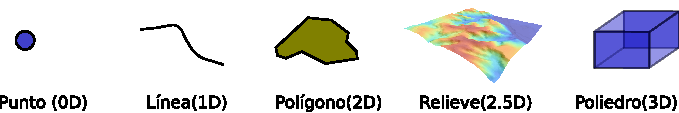
\includegraphics[width=\textwidth]{Datos/Dimensiones.pdf}
\caption{\small Dimensiones de la componente geogr�fica.}
\label{Fig:Dimensiones} 
\end{figure}


\section{Divisi�n de la informaci�n. Capas}

En un SIG, la informaci�n espacial referida a una zona de estudio \textbf{est� dividida en varios niveles}, de tal forma que, pese a coincidir sobre un mismo emplazamiento, la informaci�n sobre distintas variables se encuentra recogida de forma independiente. Es decir, en funci�n de la componente tem�tica se establecen distintos bloques de datos espaciales. Cada uno de estos bloques tem�ticos se conoce como \textbf{capa} (Figura \ref{Fig:Concepto_capa}). 

\begin{figure}[!hbt] 
\centering
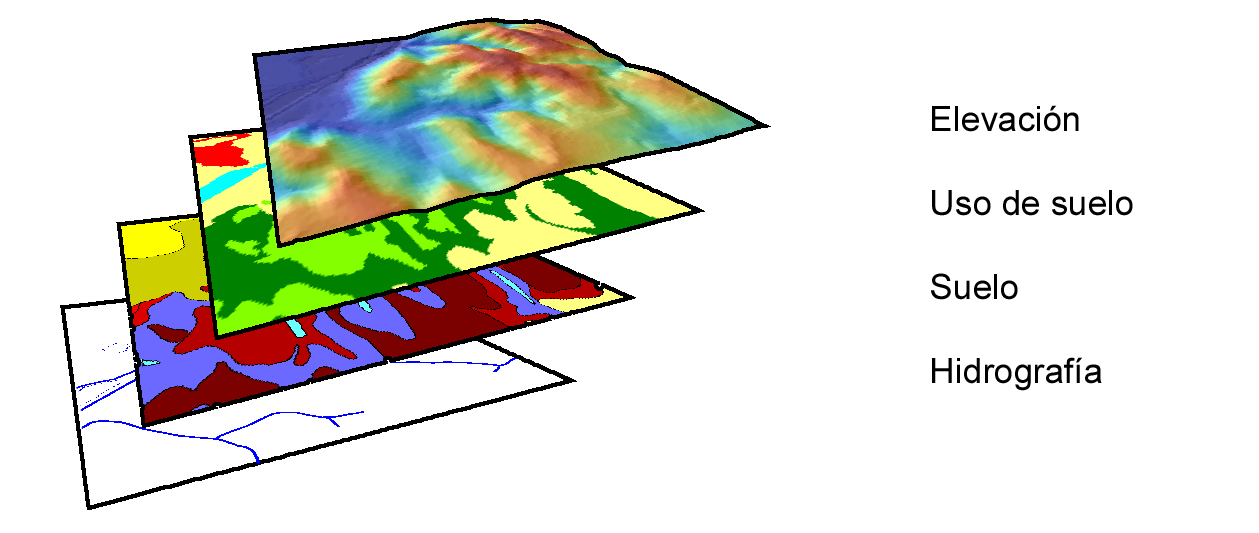
\includegraphics[width=\textwidth]{Datos/Concepto_capa.png}
\caption{\small Concepto de \emph{capa} de informaci�n geogr�fica dentro de un SIG.}
\label{Fig:Concepto_capa} 
\end{figure}

El concepto de capa es imprescindible para comprender todo SIG, y  favorece la correcta estructuraci�n de la informaci�n y el trabajo con ella. Toda la informaci�n geogr�fica con que trabajemos en un SIG va a ser en forma de capas. Cada una de ellas puede abrirse de forma independiente en un SIG y utilizarse por s� misma o en conjunto con otras.

Con la cartograf�a cl�sica, no es posible (o resulta dif�cil e impreciso) combinar distintos tipos de informaci�n, como por ejemplo la contenida en un mapa topogr�fico y la existente en un mapa de tipos de suelo y otro de vegetaci�n potencial. En el caso de un SIG, los distintos tipos de informaci�n se pueden combinar de forma sencilla y limpia, y no aparecen los mismos problemas.

La relevancia del concepto de capa como elemento fundamental de un SIG es enorme, pues constituye el marco b�sico sobre el que se van a llevar a cabo gran parte de las operaciones. Por ejemplo, vimos en el apartado dedicado a la generalizaci�n cartogr�fica c�mo en un SIG podemos utilizar diferentes <<versiones>> de los datos correspondientes a una zona concreta, y representar una u otra de ellas en funci�n de la escala de trabajo. Estas versiones se almacenar�n como distintas capas. La capa es as� la unidad fundamental no solo en t�rminos de un �rea dada, sino tambi�n de una escala concreta, y permite una divisi�n de los datos �ptima a todos los efectos.


La separaci�n de la informaci�n en capas evita asimismo la redundancia de datos, ya que cada capa contiene un tipo de informaci�n concreto. En un mapa cl�sico se presentan siempre varias variables, algunas de ellas presentes con car�cter general, tales como nombres de ciudades principales o v�as m�s importantes de comunicaci�n. En un SIG, al encontrarse estas variables separadas en sus correspondientes capas, es el usuario quien las combina.

El trabajo con capas permite, por tanto, una estructura \textbf{m�s organizada} y una \textbf{mayor atomizaci�n} de los datos, con las consecuentes ventajas en el almacenamiento, manejo y funcionalidad que esto conlleva.


Adem�s de dividir la informaci�n geogr�fica en capas de acuerdo con su contenido, tambi�n dividimos esta con criterios puramente espaciales, <<cort�ndola>> en unidades menores que ocupen una regi�n de amplitud m�s reducida. Este es un procedimiento similar al que encontramos en un mapa impreso, ya que el territorio de un pa�s se encuentra cartografiado en diferentes \emph{hojas}. 

La principal cualidad de un SIG para integrar de forma transparente datos correspondientes a zonas distintas y formar un mosaico �nico es la \textbf{separaci�n que existe entre datos y visualizaci�n}. Los datos son la base de la visualizaci�n, pero en un SIG estos elementos conforman partes del sistema bien diferenciadas. Esto quiere decir que los datos se emplean para crear un resultado visual pero en s� mismos no contienen valores relativos a esa visualizaci�n.

De este modo, es posible combinar los datos y despu�s representarlos en su conjunto. Un proceso as� no puede realizarse con un mapa ya impreso, pues este contiene ya elementos de visualizaci�n e incluso componentes cartogr�ficos tales como una flecha indicando el Norte, una leyenda o una escala. Por ello, aunque puedan combinarse, realmente no se <<funde>> la informaci�n de cada uno de los mapas para conformar uno �nico. En un SIG, por el contrario, la visualizaci�n de cuatro o m�s bloques de datos puede ser id�ntica a la que obtendr�a si todos esos datos constituyeran un �nico bloque. 

\section{Modelos para la informaci�n geogr�fica}

El proceso de convertir un �rea geogr�fica y la informaci�n acerca de ella en un dato susceptible de ser incorporado a un SIG puede dividirse en tres fases:

\begin{itemize}
 \item Establecimiento de un \textbf{modelo geogr�fico}. Es decir, un modelo conceptual de la realidad geogr�fica y su comportamiento.
\item Establecimiento de un \textbf{modelo de representaci�n}. Es decir, una forma de recoger el anterior modelo conceptual y sus caracter�sticas propias, reduci�ndolo a una serie finita de elementos.
\item Establecimiento de un \textbf{modelo de almacenamiento}. Es decir, un esquema de c�mo almacenar los distintos elementos del modelo de representaci�n.
\end{itemize}
\index{Modelo!geogr�fico}\index{Modelo!de representacion}\index{Modelo!de almacenamiento}



Por su mayor importancia, nos centraremos en los modelos de representaci�n. Los modelos de representaci�n que se utilizan principalmente en un SIG son dos: \textbf{modelo raster} y \textbf{modelo vectorial}. Las capas que utilizan estos modelos se conocen como \textbf{capas raster} y \textbf{capas vectoriales}, y esta es la terminolog�a habitual en el �mbito de los SIG para referirse a la naturaleza de una determinada capa. 

\subsection{Modelo r�ster}

El modelo r�ster se basa en una \textbf{divisi�n sistem�tica} del espacio. Todo el espacio queda cubierto y caracterizado como un conjunto de unidades elementales, cada una de ellas con un valor asociado.  

Lo m�s habitual es una divisi�n en una malla de \textbf{celdas cuadradas} o rectangulares. Conociendo la orientaci�n de la malla y las dimensiones de cada una de las celdas, as� como las coordenadas de al menos una de ellas, es posible conocer las coordenadas del resto en virtud de su \textbf{estructura regular}. Con esto, conocemos los valores de la variable en todos los puntos del espacio cubierto por la capa. El \textbf{tama�o de celda} es un par�metro relacionado con la escala de trabajo de la capa, ya que define la resoluci�n de esta y est� en funci�n de la precisi�n con que se han tomado los datos correspondientes.


La figura \ref{Fig:Raster_closeup} muestra un ejemplo de una malla r�ster.

\begin{figure}[!hbt]   
\centering
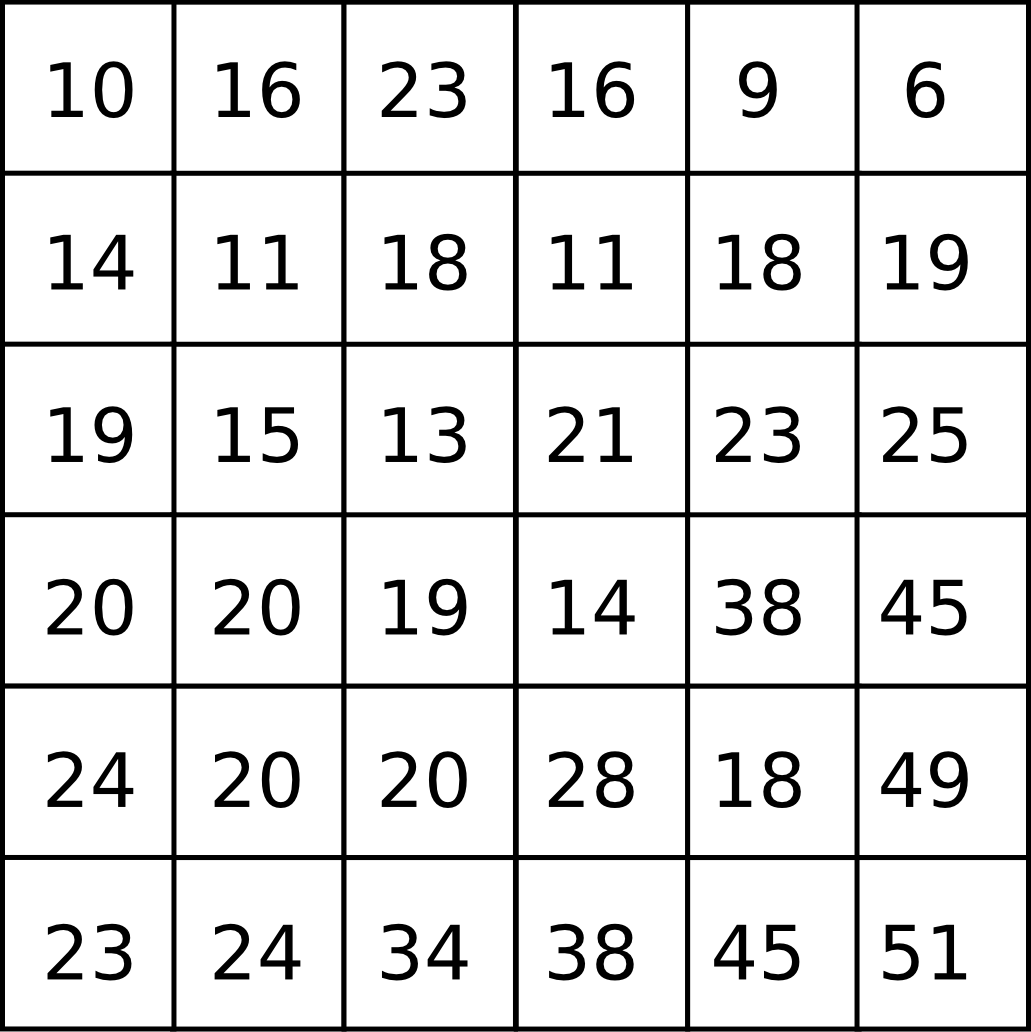
\includegraphics[width=.4\textwidth]{Datos/Raster_closeup.png}
\caption{\small Celdas de una malla r�ster con sus valores asociados.}
\label{Fig:Raster_closeup} 
\end{figure}

El n�mero de valores distintos recogidos para cada celda coincide con el n�mero de las denominadas \textbf{bandas}. Una banda contiene un �nico valor en una capa raster. Puede entenderse una capa raster de m�s de una banda como un conjunto de capas (cada banda ser�a una subcapa de ese conjunto), teniendo en todas ellas la malla de celdas las mismas caracter�sticas espaciales, y presentandose el conjunto como un �nico elemento. 

El ejemplo m�s claro de uso del modelo raster lo encontramos en las im�genes. Una imagen digital se compone de una malla de elementos (denominados \textbf{p�xeles}, cada uno de los cuales tiene un color asociado). El conjunto de estos p�xeles forman la imagen completa. Lo m�s habitual es que las im�genes contengan 3 bandas, correspondientes a las intensidades de los colores rojo, verde y azul, las cuales al combinarse permiten obtener el color de cada p�xel.

Otro uso habitual del modelo raster es en los denominados \textbf{Modelos Digitales de Elevaciones} (MDE), que recogen la topograf�a de un terreno. 

De forma general, los valores de una capa r�ster, en cualquiera de sus bandas, son \textbf{casi exclusivamente num�ricos}, no estando los SIG preparados para manejar otro tipo de valores en la componente tem�tica de una capa r�ster. De esta forma, una capa raster puede equipararse al concepto matem�tico de una \textbf{matriz}, con las ventajas que ello supone para aplicar sobre ella herramientas matem�ticas a la hora de su an�lisis.

\subsection{Modelo vectorial}


El otro modelo principal de representaci�n es el modelo vectorial. En este modelo, no existen unidades fundamentales que dividen la zona recogida, sino que se recoge la variabilidad y caracter�sticas de esta mediante \textbf{entidades}, para cada una de las cuales dichas caracter�sticas son constantes. Las entidades se componen de \textbf{primitivas geom�tricas}, y estas pueden ser de tres tipos: \textbf{puntos, l�neas} y \textbf{pol�gonos} (Figura \ref{Fig:Primitivas_vectoriales}).

\begin{figure}[!hbt]   
\centering
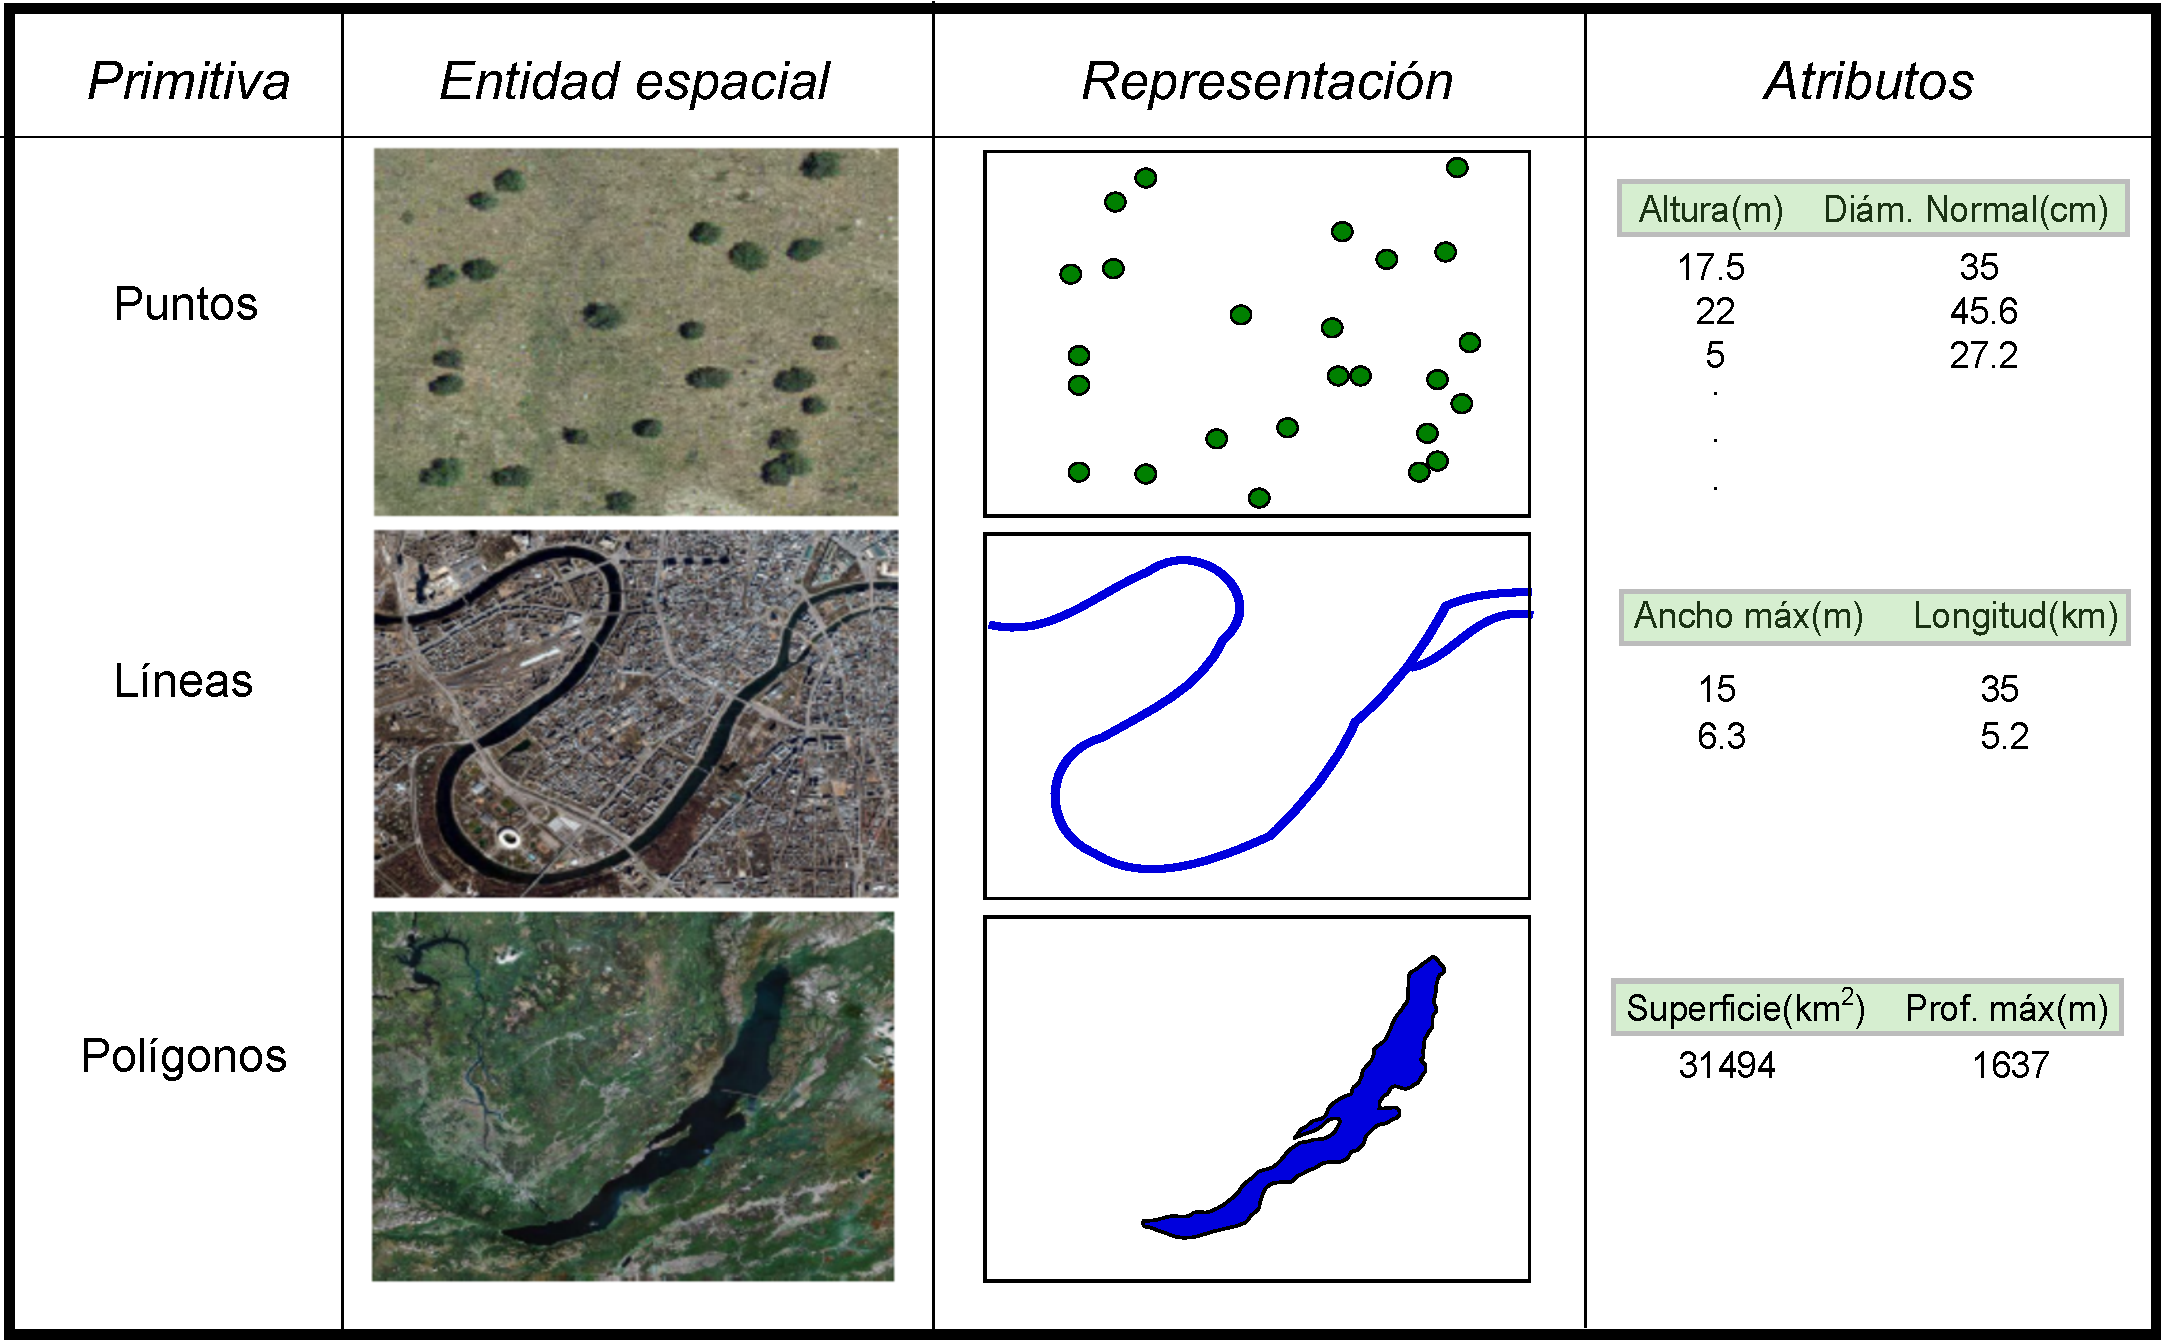
\includegraphics[width=\textwidth]{Datos/Primitivas_vectoriales.pdf}
\caption{\small Primitivas geom�tricas en el modelo de representaci�n vectorial y ejemplos particulares de cada una de ellas con atributos asociados}
\label{Fig:Primitivas_vectoriales} 
\end{figure}

Utilizando puntos, l�neas o pol�gonos, puede modelizarse el espacio geogr�fico si se asocia a estas geometr�as una serie de valores definitorios. Una entidad puede tener \textbf{varias primitivas}. Por ejemplo, en una capa de pa�ses, necesitar�amos varios conjuntos para representar Espa�a si queremos incluir tanto la peninsula como las islas que la forman. Todos estos pol�gonos constituyen una �nica entidad, ya que todos pertenecen al mismo pa�s y tendr�n el mismo conjunto de valores asociados.

A la hora de definir las formas geom�tricas b�sicas, todas ellas pueden en �ltima instancia \textbf{reducirse a puntos}. As�, las l�neas son un conjunto de puntos interconectados en un determinado orden, y los pol�gonos son l�neas cerradas, tambi�n expresables por tanto como una serie de puntos. Todo elemento del espacio geogr�fico queda definido, pues, por una serie de puntos que determinan sus propiedades espaciales y una serie de valores asociados.

Dentro de un SIG, una capa vectorial puede contener \textbf{un �nico tipo de primitiva}. As�, tenemos capas vectoriales de puntos, de l�neas y de pol�gonos, respectivamente. Una variable puede recogerse con varios tipos de primitivas (por ejemplo, puede indicarse una ciudad con un punto o con un pol�gono que delimite su per�metro), y la elecci�n de uno u otro tipo de geometr�a ha de ser funci�n del tipo de fen�meno que se pretende modelizar o la precisi�n necesaria, entre otros factores. 

La componente tem�tica en el modelo vectorial se establece mediante los denominados \textbf{atributos}, que suelen ser m�ltiples, a diferencia de lo que sucede en el modelo raster, donde lo habitual es tener un �nico valor para cada celda. Los atributos de una capa vectorial pueden contener informaci�n de cualqueir clase, siendo m�s vers�tiles que en el caso de las capas r�ster, donde ya vimos que se maneja �nicamente informaci�n num�rica. Por su estructura particular (series de atributos asociados a una entidad), la componente tem�tica en el modelo vectorial se presta especialmente a representarse en tablas y almacenarse en una \textbf{base de datos}, y puede analizarse independientemente de la componente espacial. 

Un elemento particular del modelo de representaci�n vectorial es la \textbf{topolog�a}.  Una capa vectorial contiene topolog�a si en ella se almacenan de alg�n modo las relaciones espaciales que existen entre sus elementos. Disponer de topolog�a en una capa vectorial es de gran importancia a la hora de llevar a cabo ciertos tipos de an�lisis, as� como procedimientos tales como la edici�n de los propios datos geogr�ficos. 

\begin{figure}[!hbt]   
\centering
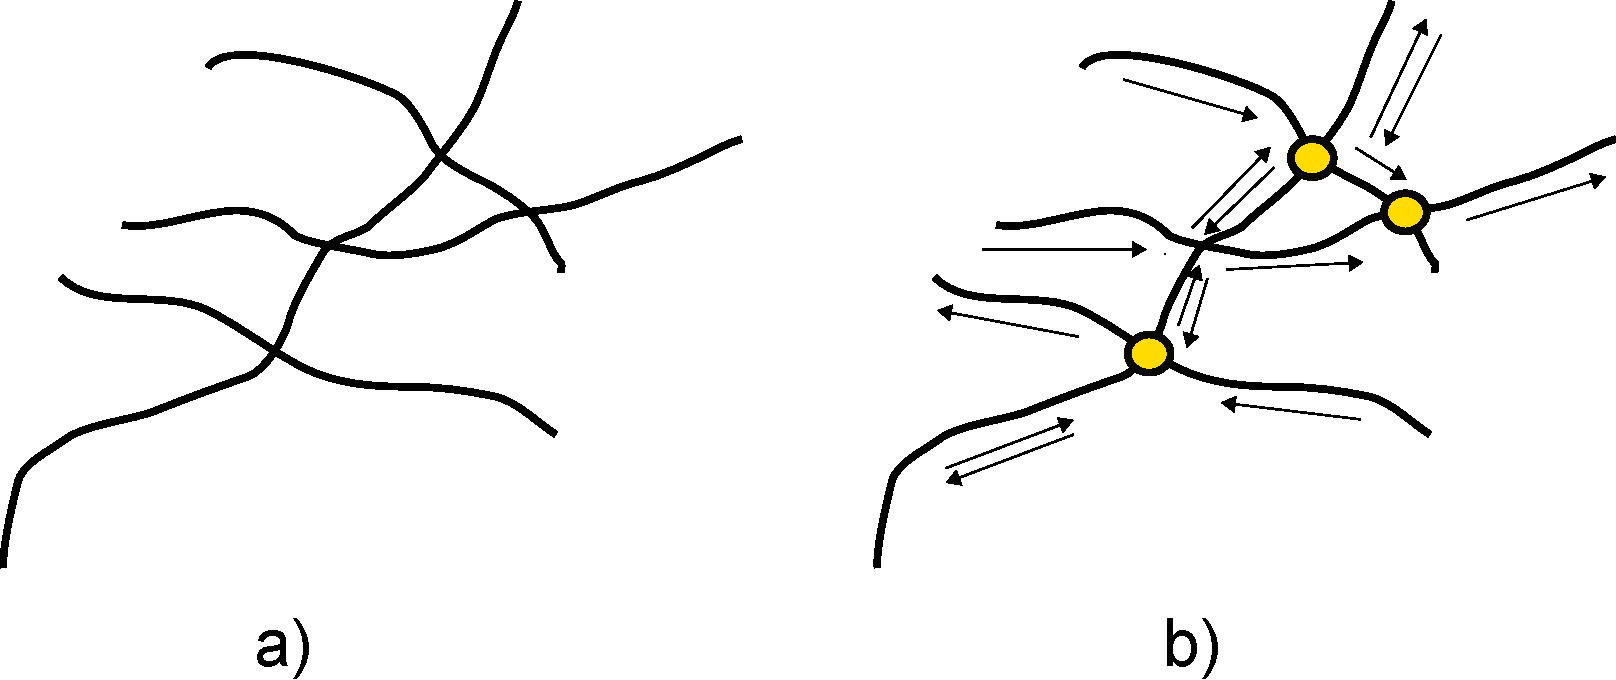
\includegraphics[width=.8\columnwidth]{Datos/Topologia_vias.pdf}
\caption{\small Capa de v�as de comunicaci�n sin topolog�a (a) o con ella (b). Los puntos en este segundo caso indican conexiones entre vias, y son una representaci�n visible de la topolog�a existente. }
\label{Fig:Topologia_vias} 
\end{figure}

Aunque la mayor�a de operaciones con una capa vectorial pueden llevarse a cabo en ausencia de topolog�a, algunas de ellas como el \textbf{an�lisis de redes} no se pueden llevar a cabo sin topolog�a. Si pensamos en una capa de v�as sobre la que desarrollar ese an�lisis de redes, un mero conjunto de elementos geom�tricos (l�neas en este caso), no nos da informaci�n sobre los posibles enlaces entre las v�as que quedan representadas. Los puntos donde se cruzan dos v�as pueden ser cruces o rotondas (es decir, puede pasarse de una v�a a otra, existiendo conexi�n entre ellas), o bien pasos elevados o subterr�neos donde una de las v�as pasa por encima de la otra (y por tanto no existe comunicaci�n entre ambas). Las circunstancias son muy distintas en funci�n del tipo de cruce que exista, y por ello es imprescindible conocer esta informaci�n para efectuar un an�lisis de redes correcto (Figura \ref{Fig:Topologia_vias})




El almacenamiento de entidades basado en una mera lista de coordenadas de cada entidad, sin topolog�a,  se conoce popularmente como \emph{spaghetti}, pues si pensamos en una capa de lineas sin topolog�a que se entrecruzan en el espacio, esta se asemejan en cierta forma a un ca�tico plato de \emph{spaguettis} sin orden ni relaci�n entre ellos.


\subsection{Raster \emph{vs} vectorial}


Tanto el modelo raster como el vectorial pueden emplearse para recoger \textbf{cualquier tipo de informaci�n}. La figura \ref{Fig:Esquemas_modelos_representacion} muestra un ejemplo de esto, representando una capa de v�as seg�n ambos modelos. Otro ejemplo para mostrar esto lo encontrarmos en las capas de elevaciones, que ya hemos visto que suelen recogerse en capas raster, en especial si se va a desarrollar sobre ellas alg�n tipo de an�lisis. No obstante, pueden recogerse tambi�n como una capa vectorial de puntos (este es una caso habitual si se obtienen los datos de un levantamiento topogr�fico), o bien como una capa de l�neas que contenga \textbf{curvas de nivel}, entre otras opciones.

\begin{figure}[!hbt]   
\centering
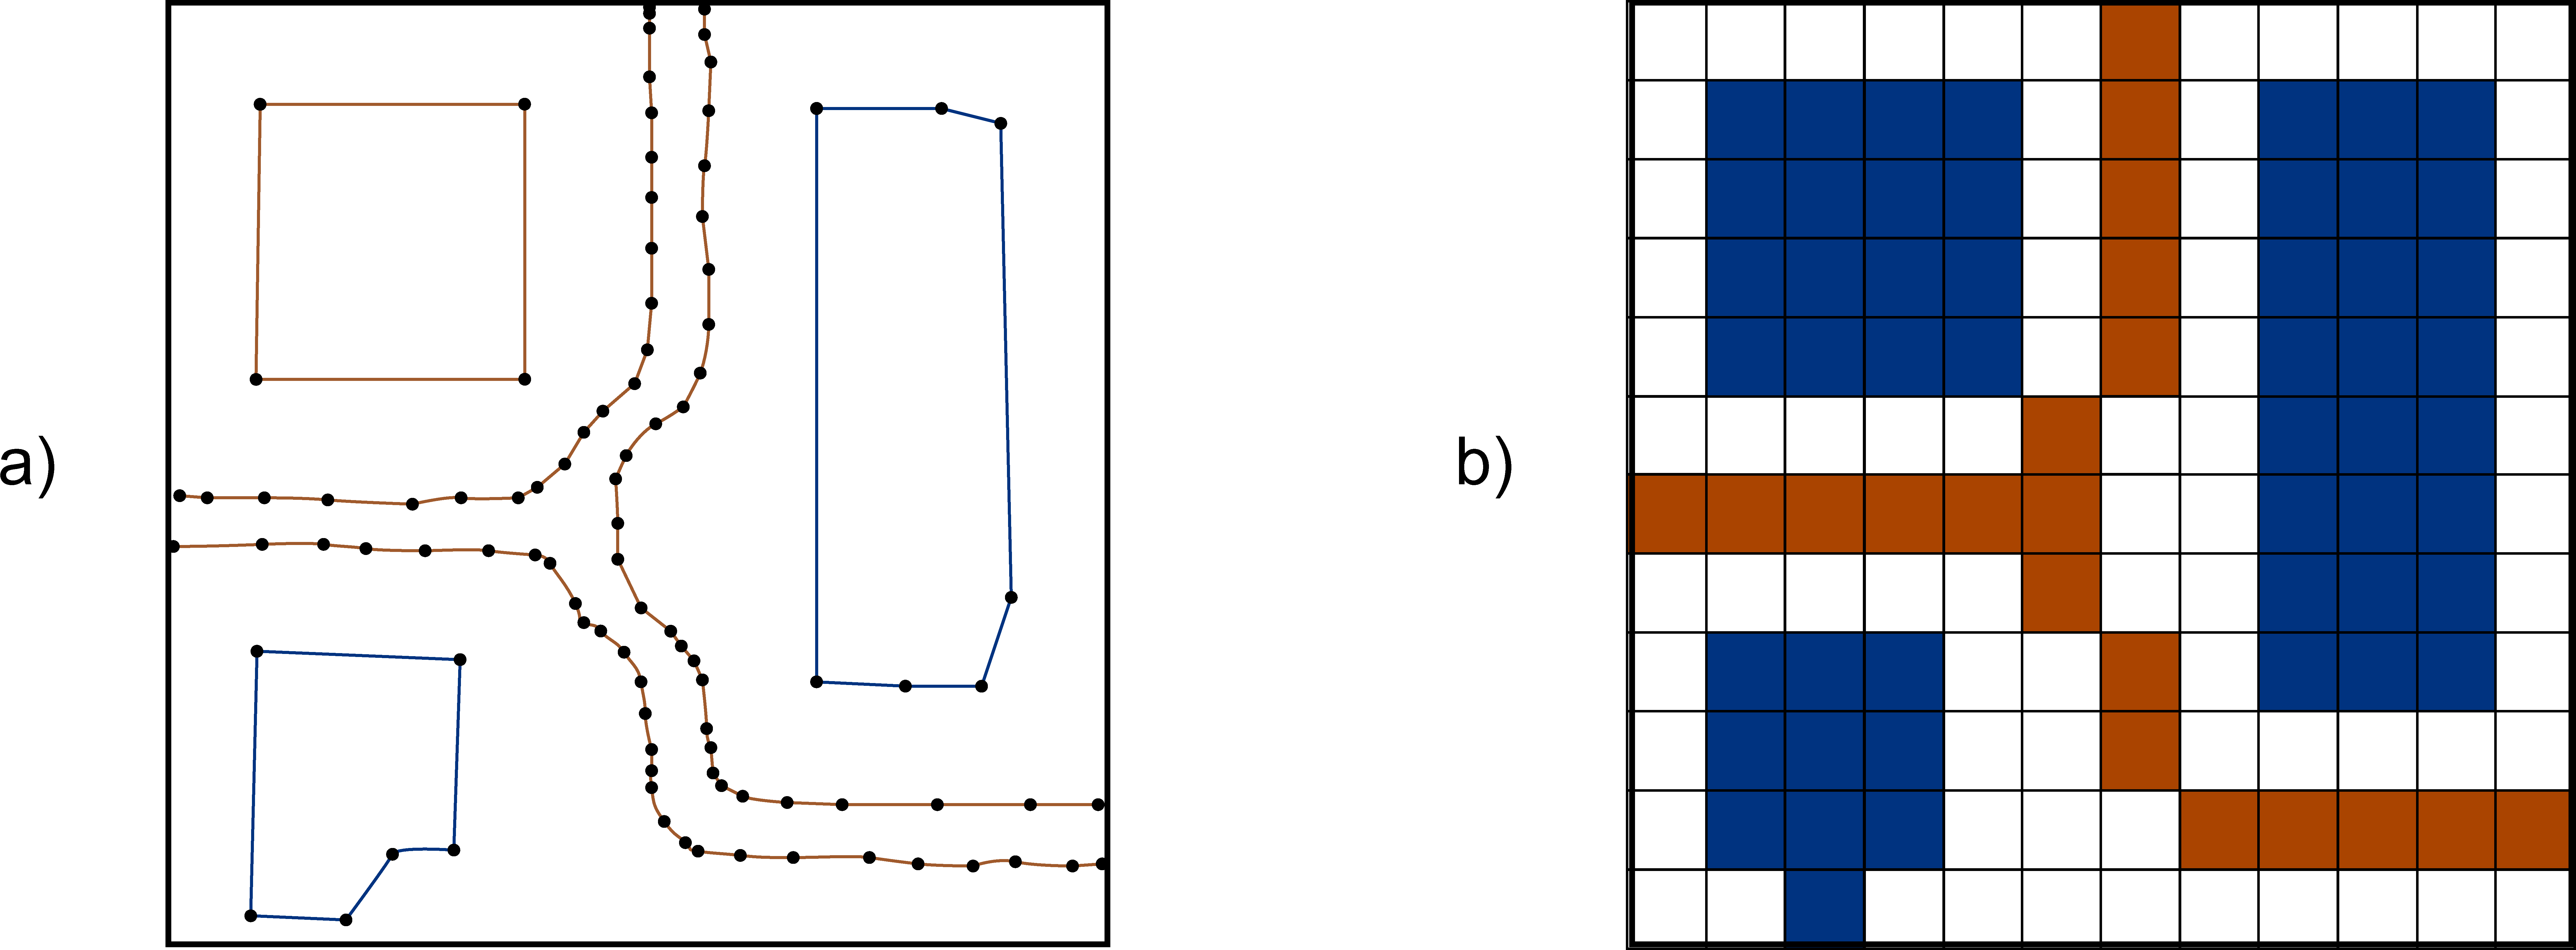
\includegraphics[width=\textwidth]{Datos/Esquemas_modelos_representacion.pdf}
\caption{\small Comparaci�n entre los esquemas del modelo de representaci�n vectorial (a) y r�ster (b).}
\label{Fig:Esquemas_modelos_representacion} 
\end{figure}


Resulta obvio que las diferencias entre los modelos r�ster y vectorial son muy notables, y que cada uno de ellos posee sus propias ventajas e inconvenientes. 
Algunos aspectos a los cuales puede atenderse para comparar uno y otro modelo son los siguientes:

\begin{itemize}
\item \textbf{Planteamiento}. El modelo r�ster hace m�s �nfasis en aquella caracter�stica del espacio que analizamos (\emph{qu�} y \emph{c�mo}), mientras que el modelo vectorial da prioridad a la localizaci�n de dicha caracter�stica (\emph{d�nde})
 \item \textbf{Precisi�n}. El modelo r�ster tiene su precisi�n limitada por el tama�o de celda. Las entidades menores que dicho tama�o de celda no pueden recogerse, y la variaci�n espacial que sucede dentro del espacio de la celda tampoco. 

Asimismo, existe una imprecisi�n en las formas. El detalle con el que puede recogerse la forma de una entidad geogr�fica seg�n el modelo vectorial es, en la pr�ctica, ilimitado, mientras que, como puede verse en la imagen \ref{Fig:Imprecision_raster}, el modelo r�ster restringe las formas a �ngulos rectos, ya que la unidad base es un cuadrado. 

\begin{figure}[!hbt]   
\centering
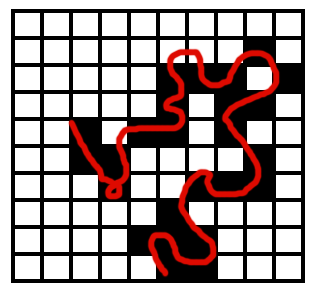
\includegraphics[width=.4\columnwidth]{Datos/Imprecision_raster.png}
\caption{\small Imprecisi�n de forma en el modelo de representaci�n r�ster. La divisi�n del espacio en unidades cuadradas impide la representaci�n fiel de entidades tales como curvas.}
\label{Fig:Imprecision_raster} 
\end{figure}

\item \textbf{Complejidad}. La regularidad y sistematicidad de las mallas r�ster hacen sencillo el implementar algoritmos de an�lisis, muy especialmente aquellos que implican el uso combinado de varias capas. Por el contrario, la irregularidad espacial de las capas vectoriales hace que la implementaci�n de los mismos algoritmos sea sumamente m�s compleja si se trabaja con estas capas.


\end{itemize}

No existe un modelo de representaci�n id�neo de forma global, sino que esta idoneidad depende de muchos factores, como por ejemplo:

\begin{itemize}
 \item \textbf{Tipo de variable o fen�meno a recoger}. Las variables \textbf{continuas} tales como la elevaci�n es m�s adecuado en general recogerlas en capas raster, para as� facilitar su an�lisis, mientras que las variables \textbf{discretas} es preferible almacenarlas como capas vectoriales.
\item \textbf{Tipo de an�lisis o tarea a realizar sobre dicha variable}. El uso que demos a una capa tem�tica condiciona en gran medida el modelo de datos id�neo. Por ejemplo, en el caso de una capa de elevaciones, su an�lisis se lleva mejor a cabo si esta informaci�n est� recogida seg�n el modelo r�ster. Sin embargo, si el objetivo principal es la visualizaci�n de esa elevaci�n en conjunto con otras variables, unas curvas de nivel pueden resultar m�s adecuadas, ya que, entre otras cosas, no interfieren tanto con otros elementos a la hora de dise�ar un mapa con todas esas variables.
\item \textbf{Contexto de trabajo}. Por ejemplo, si queremos trabajar con im�genes, esto nos condiciona al empleo de datos r�ster, ya que resulta mucho m�s sencillo combinarlos con las im�genes, las cuales siempre se presentan como capas r�ster. 
\end{itemize}


Existen procedimientos para \textbf{convertir} entre los formatos r�ster y vectorial, de forma que el disponer de datos en un modelo de representaci�n particular no implica que debamos desarrollar nuestro trabajo sobre dichos datos directamente, sino que podemos efectuar previamente una conversi�n.


\pagestyle{empty}

\chapter{Fuentes principales de datos espaciales}
\label{Fuentes_datos}

\pagestyle{fancy}


No hace tanto tiempo, toda la informaci�n que se manejaba dentro de un SIG ten�a su origen en un mapa en papel, el cual deb�a \emph{prepararse} para adaptarse a la naturaleza propia del SIG. El dato geogr�fico se obten�a a partir de la \textbf{digitalizaci�n} de cartograf�a, es decir, convertir los datos geogr�ficos en formato impreso en datos en formato digital que un SIG pudiera manejar. 

Un SIG implica una aplicaci�n inform�tica, y esta se alimenta en �ltima instancia exclusivamente de datos digitales. Los datos geogr�ficos digitales tienen una serie de ventajas frente a los anal�gicos (adem�s del mero hecho de que podemos incorporarlos a nuestro SIG), y suponen, como sucede en muchos otros campos, un salto cualitativo importante. Entre estas ventajas, que son a su vez comunes a otros �mbitos,  destacan la sencillez de actualizaci�n, la facilidad de distribuci�n (en especial con la aparici�n de Internet), el menor espacio f�sico necesario para su almacenamiento, la facilidad y precisi�n del an�lisis, y la facilidad de mantenimiento (el dato digital no se degrada, lo que se degrada es su soporte, pero es sencillo replicar el dato sin p�rdida de calidad)

Hoy en d�a las t�cnicas de adquisici�n de datos han evolucionado y permiten crear datos que pueden ser directamente integrados en un SIG. Distinguimos as� \textbf{fuentes de datos primarias} y \textbf{secundarias}. 

Las fuentes de datos primarias son aquellas cuyos datos podemos emplear en un SIG, ya que estos, en su forma original, ya son susceptibles de ser sometidos a las operaciones de manejo y an�lisis que incorporan los SIG. Por su parte, las fuentes de datos secundarias generan datos que no pueden emplearse en un SIG sin un proceso de adaptaci�n previo, siendo el dato derivado el que utilizamos en un SIG, no el original. 

En este cap�tulo, veremos las distintas fuentes de datos con las que podemos trabajar un en SIG.


\section{Teledetecci�n}\index{Teledetecci�n}

La primera fuente de datos que trataremos en este cap�tulo es la teledetecci�n. Entendemos por teledetecci�n el estudio y medida de las caracter�sticas de una serie de objetos (en nuestro caso elementos de la superficie terrestre) sin que exista contacto f�sico. Para ello, se miden las perturbaciones que el objeto provoca en su entorno, principalmente las de tipo electromagn�tico.

Un sistema de teledetecci�n cuenta con los siguientes elementos (Figura \ref{Fig:Elementos_teledeteccion}):

\begin{figure}[!hbt]   
\centering
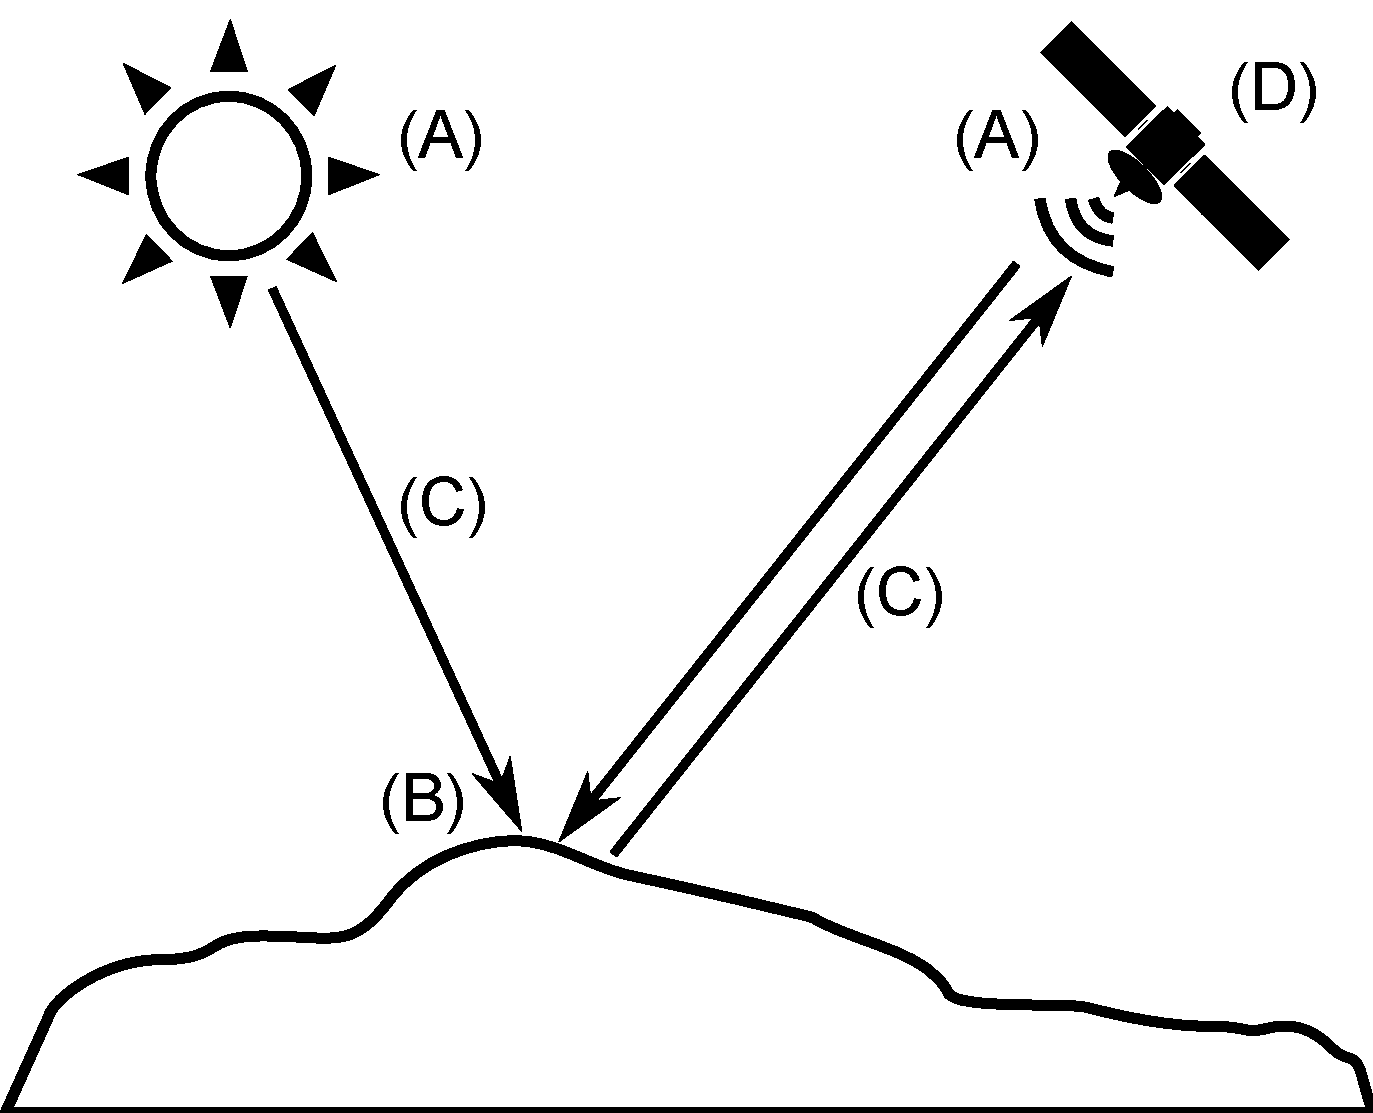
\includegraphics[width=.6\textwidth]{Fuentes_datos/Elementos_teledeteccion.pdf}
\caption{\small Esquema de un sistema de teledetecci�n.}
\label{Fig:Elementos_teledeteccion} 
\end{figure}


\begin{itemize}
	\item \textbf{Una fuente de radiaci�n (A)}\index{Fuente de radiaci�n}. Puede ser de origen natural o artificial. La radiaci�n emitida por dicha fuente llega al terreno y sufre una perturbaci�n causada por los elementos de este, siendo esta perturbaci�n el objeto de estudio de la teledetecci�n. Los propios objetos pueden ser tambi�n emisores ellos mismos de radiaci�n.
	\item \textbf{Unos objetos (B) que interaccionan con la radiaci�n} o la emiten, seg�n lo anterior.
	\item \textbf{Una atm�sfera (C)} por la que se desplaza la radiaci�n, tanto desde la fuente hasta el objeto como desde el objeto hasta el receptor. La atm�sfera tambi�n interact�a con la radiaci�n, introduciendo igualmente perturbaciones en ella.
	\item \textbf{Un receptor (D) que recoge la radiaci�n} una vez esta ha sido perturbada o emitida por los objetos. El receptor va a generar como producto final una imagen (en t�rminos de un SIG, una capa r�ster), en cuyas celdas o p�xeles se va a contener un valor que indica la intensidad de la radiaci�n. Estos valores son valores enteros que indican el nivel de dicha radiaci�n dentro de una escala definida (habitualmente valores entre 1 y 256), y se conocen dentro del �mbito de la teledetecci�n como \textbf{Niveles Digitales}.
\end{itemize}

A lo largo de este apartado veremos con detalle estos elementos. Para estudiar los dos primeros, estudiaremos los fundamentos f�sicos relativos a la radiaci�n y a la la interacci�n entre esta y la materia, mientras que para el estudio del sistema receptor analizaremos los elementos de este en dos componentes por separado: sensores y plataformas. 

La interacci�n de la atm�sfera interesa de cara a eliminar su efecto, ya que lo que resulta de inter�s en general son los objetos en la superficie terrestre, no la atm�sfera como tal. Eliminar esta influencia de la atm�sfera es parte de los procesos posteriores que se realizan con la imagen, y que se detallan en los cap�tulos dedicados al an�lisis de im�genes en lugar de en este.

\subsection{Fundamentos f�sicos}

La radiaci�n electromagn�tica es producto de las alteraciones en los campos el�ctrico y magn�tico, las cuales generan ondas correspondientes a cada uno de los campos magn�tico y el�ctrico. Estas ondas se desplazan a la velocidad de la luz, y se pueden describir con los par�metros habituales, tales como la longitud de onda o la frecuencia. El rango de longitudes de onda cubierta por la radiaci�n electromagn�tica se conoce como \textbf{espectro electromagn�tico}.

El espectro se subdivide en regiones en funci�n de su longitud de onda, tales como (de menor a mayor longitud de onda) los rayos $\gamma$, los rayos X, la regi�n ultravioleta, la regi�n visible, la regi�n infraroja, o las microondas  

La radiaci�n emitida por una fuente de radiaci�n es alterada por la presencia de los distintos objetos, ya que estos \textbf{absorben, transmiten} o \textbf{reflejan} esta.

Estos tres fen�menos se dan en diferente proporci�n en funci�n de las caracter�sticas del objeto y de la radiaci�n. La parte que  interesa a efectos de la teledetecci�n es aquella que se refleja en el objeto, ya que esta es la que posteriormente puede recogerse y emplearse para la generaci�n de las im�genes.

Como ya se dijo en el cap�tulo \ref{Introduccion_datos}, las im�genes como capas r�ster presentan habitualmente la particularidad de tener varias bandas. En lugar de un �nico valor para cada celda, existen $n$ valores, uno por cada banda. La imagen recoge la \textbf{intensidad de la radiaci�n} dentro de una amplitud dada del espectro, y a su vez subdivide esta en distintas franjas. Los Niveles Digitales de cada banda corresponden a la intensidad dentro de una de esas franjas del espectro en particular.

Puesto que cada objeto refleja la radiaci�n de diferentes longitudes de onda de modo distinto, esto puede considerarse como una propiedad del objeto. Se tiene as� el concepto de \textbf{firma espectral}, que es la respuesta caracter�stica de un tipo de objeto dentro del espectro electromagn�tico. 


\subsection{Sensores y plataformas}

En un sistema de teledetecci�n, dos son los elementos tecnol�gicos principales que lo definen: el \textbf{sensor} y la \textbf{plataforma}. 

El sensor es el elemento que incorpora la capacidad de <<leer>> la radiaci�n electromagn�tica y registrar su intensidad dentro de la una zona concreta del espectro. Puede ir desde una simple c�mara fotogr�fica hasta un sensor m�s especializado.

Los sensores se denominan \textbf{pasivos} aprovechan las fuentes de radiaci�n existentes en la naturaleza (fundamentalmente el Sol) y se limitan a recoger la radiaci�n de dichas fuentes reflejada por los elementos del medio, o \textbf{activos} s� emiten radiaci�n, y recogen dicha radiaci�n tras ser reflejada por dichos elementos. Para entender este concepto de un modo de un modo sencillo, podemos decir que una c�mara fotogr�fica es un sensor pasivo, mientras que una camara fotogr�fica con \emph{flash} es un sensor activo. La radiaci�n emitida por los sensores activos no ha de ser necesariamente luz visible (como en el caso del flash), sino que pueden emitir en otras secciones del espectro.

Tecnolog�as como el \textbf{radar} o el \textbf{LiDAR} (similar al radar pero con pulsos de laser en lugar de ondas de radio), se basan en sensores activos. En el caso del LiDAR, permite obtener imagenes que no tiene un caracter visual, sino que contienen en sus valores la elevaci�n de los objetos, pudiendo as� emplearse para cartografiar el relieve.


La plataforma, por su parte, es el medio en el que se sit�a el sensor y desde el cual se realiza la observaci�n.  A bordo de una plataforma pueden montarse \textbf{varios sensores}.

Los dos tipos principales de plataformas son aquellas situadas \textbf{dentro de la atm�sfera} terrestre (aviones en su mayor�a) y aquellas situadas \textbf{fuera de la atm�sfera} (a bordo de sat�lites).

Los aviones tienen la ventaja de su \textbf{disponibilidad}, ya que pueden pilotarse y de este modo permiten cubrir cualquier lugar de la tierra en cualquier momento.

A diferencia de un avi�n, un sat�lite no puede dirigirse a voluntad (no puede pilotarse), y su movimiento es una caracter�stica inherente que viene definida por una serie de par�metros. Estos par�metros se conocen como \textbf{par�metros orbitales} pues definen la �rbita descrita por el sat�lite en torno a la Tierra. 

Las �rbitas pueden clasificarse en funci�n de su \textbf{eje de rotaci�n} as� como en funci�n de su \textbf{movimientos}. En este �ltimo caso tenemos �rbitas \textbf{geos�ncronas} (el sat�lite se sit�a sobre un punto fijo de la Tierra y su movimiento sigue al de rotaci�n de esta) o \textbf{helios�ncronas} (mientras el sat�lite recorre la �rbita, la Tierra efect�a su movimiento de rotaci�n, lo cual hace que a cada vuelta de la �rbita se cubran zonas distintas) 
	
	

\subsubsection{Resoluciones}

Uno de los par�metros principales que definen las propiedades de un sistema de teledetecci�n son las \emph{resoluciones}. Estas establecen el nivel de detalle de los productos que el sistema genera, determinando este en las distintas magnitudes en las que el sistema opera. Las resoluciones dependen del sensor y de la plataforma como binomio operativo, y de las caracter�sticas propias de ambos. Distinguimos cuatro resoluciones, a saber:

\begin{itemize}
	\item \textbf{Resoluci�n espacial}. Indica la dimensi�n del objeto m�s peque�o que puede distinguirse en la imagen. Es la dimensi�n real que un p�xel de la imagen tiene sobre el terreno.

	
	\item \textbf{Resoluci�n espectral}. Indica la amplitud de cada una de las regiones del espectro quqe se recogen en la imagen. La regi�n del espectro abarcada y el n�mero de bandas son los elementos que definen la resoluci�n espectral. 

	\item \textbf{Resoluci�n radiom�trica}. Para cada una de las bandas que produce un sensor (asociada esta a una determinada regi�n del espectro seg�n su resoluci�n espectral), el dato recogido, que constituye su Nivel Digital, indica la intensidad correspondiente a esa regi�n. El nivel de detalle con el que puede medirse esa intensidad es el que define la resoluci�n radiom�trica del sensor.\index{Resoluci�n!radiom�trica}
	
	\item \textbf{Resoluci�n temporal}. Indica el tiempo que tarda el sensor en volver a tomar una imagen de una misma zona.  Tiene sentido en el caso de sensores orbitales. La resoluci�n temporal depende de la altura a la que se encuentra la plataforma que monta el sensor, as� como la resoluci�n espacial. 
\end{itemize}

No resulta posible (por razones t�cnicas y te�ricas) disponer de un sensor en el cual todas las anteriores regiones sean altas. Algunos sensores priman determinadas resoluciones, mientras que otros favorecen otras distintas.

A la hora de utilizar im�genes de teledetecci�n, debe considerarse qu� tipo de resoluci�n  resulta de mayor inter�s (por ejemplo, para localizar elementos de peque�o tama�o son necesarias im�genes con alta resoluci�n especial). En base a esto, se escoger� una u otra clase de im�genes, que ser� la que ofrezca los valores de resoluci�n m�s adecuados en conjunto. La utilizaci�n simult�nea de datos de varios sensores en un proyecto es una alternativa para compensar este hecho.


\subsection{Fotogrametr�a}
\label{Fotogrametria}

\index{Fotogrametr�a}

Relacionada con la teledetecci�n, encontramos la \textbf{fotogrametr�a}. La fotogrametr�a es la t�cnica para estudiar y definir con precisi�n la forma, dimensiones y posici�n en el espacio de un objeto cualquiera, utilizando medidas realizadas sobre una o varias fotograf�as. En el campo del SIG, es de especial inter�s la \textbf{fotogrametr�a a�rea}, cuya base de trabajo tradicional son las fotograf�as a�reas, y que sirve principalmente para la creaci�n de cartograf�a de elevaciones a partir de un proceso de \textbf{restituci�n}.

En lugar de im�genes individuales, la fotogrametr�a emplea pares de im�genes, cada una de ellas tomada desde un punto distinto. Mediate estereoscop�a, resulta posible recrear el efecto que ambas im�genes tendr�an para la reconstrucci�n tridimensional de la escena, y <<enga�ar>> al cerebro del observador para que este pueda observar la escena con \textbf{volumen y profundidad}. Esto permite posteriormente conocer las formas del terreno, y a partir de ello crear las capas correspondientes, con informacion de elevaciones.

Cuando se emplean im�genes de sat�lite, los pares se pueden obtener con aquellas plataformas y sensores que permiten \textbf{variar el �ngulo de visi�n}, de modo que en la misma pasada del sat�lite se toman im�genes de una zona desde distintos puntos. 

Seg�n su enfoque, la fotogrametr�a puede ser \textbf{anal�gica}, \textbf{anal�tica} o  \textbf{digital}, siendo esta �ltima la que se basa en el trabajo con im�genes digitales dentro de un entorno computerizado, y la que mayor relaci�n tiene con los SIG. 

La fotogrametr�a requiere de una \emph{estaci�n fotogram�trica}, que en el caso digital incorpora muchos elementos propios de un SIG, as� como otros espec�ficos del trabajo fotogram�trico. Entre estos, caben destacar aquellos que permiten la generaci�n de visualizaciones con sensaci�n de profundidad, as� como los perif�ricos espec�ficos tales como ratones 3D o manivelas similares a las que presentan los restituidores anal�ticos, facilitando as� la adaptaci�n de los operarios a este tipo de estaci�n.


\section{Cartograf�a impresa. Digitalizaci�n}

Existe gran cantidad de cartograf�a en formato no digital, tales como mapas impresos o fotograf�as a�reas antiguas en formato anal�gico. 

La \textbf{digitalizaci�n} de esta cartograf�a, necesaria para su uso en un SIG, supone la creacion de capas raster o vectoriales a partir de ella. En este �ltimo caso, implica la \textbf{disgregaci�n} de la informaci�n que contiene, ya que en un mapa clasico se presentan distintas informaciones que en el uso com�n de un SIG se almacenan en capas independientes.

La digitalizaci�n implica tres etapas: el \textbf{registro o georeferenciaci�n}(Establecimiento del marco geogr�fico ---sistema de coordenadas, puntos de control, etc---, de forma que los elementos digitalizados posteriormente sean correctos), la digitalizaci�n de la compoente espacial (creaci�n de geometr�as en el caso de capas vectoriales), y la digitalizaci�n de la componente tem�tica (creaci�n de valores de celda en el caso de capas raster o de atributos en el caso vectorial).

La digitalizaci�n puede ser \textbf{manual} o \textbf{autom�tica}. En el primer caso, es un operario quien introduce los valores de los elementos digitalizados, mientras que en el segundo caso es un procedimiento automatizado el que se encarga de ello.

Para la creaci�n de capas raster, lo habitual es la digitalizaci�n autom�tica, a partir del \textbf{escaneo} del documento original.

El escaneo es el proceso de digitalizaci�n que convierte una imagen impresa (anal�gica) en una imagen digital. Dentro de un SIG, se emplea para digitalizar tanto mapas como fotograf�as a�reas, y su resultado es una capa r�ster. 

Aunque existen esc�neres espec�ficamente dise�ados para el trabajo con documentos cartogr�ficos, estos son dispositivos muy especializados y de muy elevado coste. Los esc�neres m�s gen�ricos, pensados para el trabajo con todo tipo de im�genes y para todo tipo de usos, pueden no obstante emplearse de igual modo para escanear tanto mapas como im�genes a�reas con resultados aceptables, utiliz�ndose con frecuencia.


Los par�metros b�sicos que definen las caracter�sticas de un esc�ner son la \textbf{resoluci�n espacial} y la \textbf{resoluci�n radiom�trica}. La primera de estas se mide habitualmente en \textbf{puntos por pulgada} y nos indica el n�mero de puntos (celdas) que el sensor es capaz de tomar por cada unidad de longitud sobre el papel. La resoluci�n radiom�trica, por su parte, indica la capacidad del sensor para distinguir entre dos colores distintos. 

En relaci�n con las resoluciones de escaneo, no deben olvidarse los fundamentos cartogr�ficos que se explicaron en un cap�tulo anterior. Trabajando con una resoluci�n m�s elevada no hace necesariamente que estemos incorporando m�s informaci�n, ya que esta puede no existir en el documento original. Tendr�amos un volumen de datos m�s elevado que el necesario para recoger toda la informaci�n del mapa.

En el caso de capas vectoriales, es m�s habitual la \textbf{digitalizaci�n manual}. En ella, un operario va definiendo las entidades, trazando las forma de estas o, en caso de ser una entidad de tipo punto, indicando su localizaci�n. 

Para llevar a cabo ese trazado de la entidad, se necesita emplear alg�n equipo que recoja la informaci�n introducida por el operador. Existen dos alternativas principales: utilizar una \textbf{tableta digitalizadora} dise�ada espec�ficamente para la digitalizaci�n, o bien digitalizar utilizando las \textbf{funciones de edici�n} de un SIG, realizando todo el proceso dentro de este y sin m�s herramientas que el propio ordenador y un dispositivo se�alador como el rat�n. En este segundo caso, la digitalizaci�n se produce sobre la pantalla, por lo que es necesario tener ya una versi�n  digital del documento (aunque no en forma de capa vectorial), la cual puede obtenerse mediante escaneo.

La digitalizaci�n autom�tica de entidades para formar una capa vectorial, conocida como \textbf{vectorizaci�n}, resulta tambi�n posible, aunque presenta m�s dificultades. El principal problema reside en la necesidad de una \textbf{adecuada preparaci�n} del documento a digitalizar, ya que las condiciones de este afectan notablemente a la calidad del resultado. La vectorizaci�n, al igual que la digitalizaci�n manual, puede llevarse a cabo mediante dispositivos especializados, o bien mediante el software apropiado, el cual se ejecuta en un ordenador y trabaja con una imagen escaneada del documento original.

Un caso particular de digitalizaci�n es la creaci�n de \textbf{capas a partir de valores o coordenadas}. Es decir, cuando no existe un mapa o documento cartogr�fico, sino simplemente una serie de datos espaciales expresados de forma alfanum�rica que son susceptibles de convertirse en una capa y emplearse as� dentro de un SIG. Este proceso se conoce como \textbf{geocodificaci�n}  e implica la asignaci�n de coordenadas a puntos de inter�s tales como muestreos de campo levantamientos topogr�ficos, inventarios de lugares donde tiene lugar un determinado fen�meno  o existe un determinado elemento, u otros como el \emph{geotagging} de fotograf�as, para asociar a estas la posici�n del enclave en el que se han tomado.

En el caso de encontrarse en formato anal�gico, estos datos pueden digitalizarse mediante la simple introducci�n manual de coordenadas a trav�s del teclado o bien mediante alg�n sistema m�s espec�fico como el escaneo del documento y el empleo de alg�n software de reconocimiento de caracteres (OCR).

En el caso de encontrarse ya en formato digital, estos datos pueden presentarse como tablas en una hoja de c�lculo, datos asociados a otro dato de cualquier tipo (como en el caso del \emph{geotagging}) o incluso simples archivo de texto. Muchos SIG incorporan m�todos para leer estos archivos y despu�s utilizar las coordenadas que contienen con el fin de crear una nueva capa, en general de puntos.



\subsection{Calidad de la digitalizaci�n}
\label{Condiciones_digitalizacion}


Uno de los aspectos m�s importantes del proceso de digitalizaci�n es la \textbf{calidad del resultado} obtenido, que debe tratar de ser lo m�s cercano posible a la calidad original de la informaci�n que se digitaliza, es decir, del mapa o imagen original. Independientemente de la precisi�n del equipo utilizado o la habilidad y experiencia del operario, la digitalizaci�n no es por completo perfecta, conteniendo siempre ciertas deficiencias y errores. 

Adem�s de los errores que puedan incorporarse en las distintas fases del proceso de digitalizaci�n (sea este del tipo que sea), hay que considerar que las fuentes originales a digitalizar tambi�n pueden incluir los suyos propios. As�, el proceso de escaneado puede incorporar distorsiones geom�tricas, pero es posible que el mapa o fotograf�a a�rea de partida tambi�n presente alguna distorsi�n como consecuencia de su deterioro, m�s patente cuanto m�s antigua sea esta. 

La informaci�n contenida en el documento cartogr�fico puede tambi�n contener elementos problem�ticos de cara a obtener un producto de calidad, que pueden ir desde l�neas borradas total o parcialmente a manchas en el propio mapa derivadas de su uso habitual.

Dentro de los errores que aparecen como consecuencia de la digitalizaci�n en s�, un tipo importante de ellos son las \textbf{discrepancias y coincidencias imperfectas} entre las distintas entidades, tal como las que se muestran en la figura \ref{Fig:Imprecisiones_digitalizacion}

\begin{figure}[!hbt]   
\centering
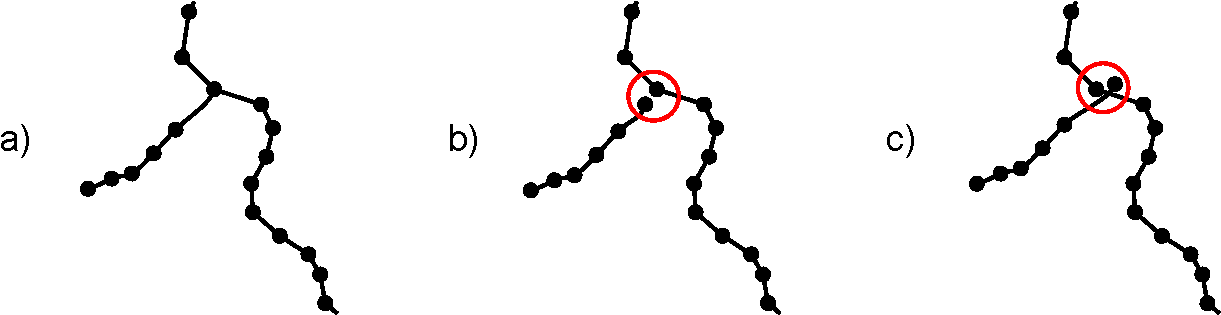
\includegraphics[width=.8\textwidth]{Fuentes_datos/Imprecisiones_digitalizacion.pdf}
\caption{\small Errores derivados del proceso de digitalizaci�n. a) Versi�n correcta, con nodos coincidentes. b) y c) Versiones con errores que causan una falsa desconexi�n entre las l�neas.}
\label{Fig:Imprecisiones_digitalizacion} 
\end{figure}


Debido a esto, las capacidades de edici�n de los SIG incorporan funcionalidades que permiten evitar estos errores en el momento de la digitalizaci�n, ayudando al operario en su tarea y permiti�ndole alcanzar una exactitud y precisi�n imposible de lograr sin estas funcionalidades. Entre ellas, es especialmente importante el establecimiento de tolerancias y ajuste autom�tico en funci�n de ellas (esto se conoce con el t�rmino ingles \textbf{snapping}), que ayudan a garantizar la coincidencia entre los distintos v�rtices. 


El hecho de que exista una completa coincidencia es especialmente importante cuando la capa vectorial que se digitaliza contiene \textbf{informaci�n topol�gica}. La topolog�a exige que la coincidencia sea correcta y defina perfectamente la relaci�n entre las entidades. La digitalizaci�n de entidades, en caso de querer recoger su topolog�a, debe realizarse siguiendo reglas adicionales tales como la digitalizaci�n una �nica vez de los lados comunes de pol�gonos. Debe, asimismo, recoger informaci�n adicional, como por ejemplo la necesaria para la definici�n de nodos en los cruces entre l�neas cuando existe relaci�n entre estas.


\section{GPS}
\label{GPS}

Uno de los hitos en la aparici�n de nuevas fuentes de datos geogr�ficos es la aparici�n de los \textbf{Sistemas Globales de Navegaci�n por Sat�lite}. Se trata de sistemas que permiten \textbf{conocer en todo momento y en cualquier punto del globo la localizaci�n exacta de dicho punto} con un margen de error del orden de unos pocos metros o menos. Para ello, se basan en el env�o de se�ales entre un dispositivo situado en el punto concreto y una red de sat�lites, pudiendo establecerse la posici�n exacta mediante las caracter�sticas de dicha transmisi�n.

El ejemplo m�s extendido de estos sistemas es el \textbf{Sistema de Posicionamiento Global} (Global Positioning System, o \textbf{GPS}). El GPS cuenta con una constelacion de 24 sat�lites activos, as� como estaciones terrestres que los controlan, y su funcionamiento se basa en la \textbf{triangulaci�n de la posici�n} de una unidad receptora, mediante las se�ales procedentes de un cierto n�mero de sat�lites. Esta triangulaci�n se basa en distancias entre la unidad receptora y dichos satelites, las cuales se calculan mediante diversos mecanismos. La posici�n se calcula no �nicamente en sus coordenadas \emph{x} e \emph{y}, sino tambi�n en \emph{z}, es decir en elevaci�n. El sistema GPS emplea como sistema geod�sico de referencia el WGS84.

.



El dise�o de la red de sat�lites est� pensado para garantizar que en cualquier punto de la superficie terrestre y en cualquier momento, un receptor puede localizar el n�mero necesario de sat�lites para obtener con exactitud su precisi�n. 

Existen \textbf{numerosas fuentes de error} que causa desviaciones apreciables en el calculo de coordenadas mediante GPS. Entre ellas destacan los errores en la posici�n de los sat�lites, errores por el rebote de la se�al en otros con anterioridad a alcanzar el receptor, errores por el paso de la se�al por la atm�sfera, as� como los de precisi�n de los relojes empleados para el c�lculo de distancias. La \textbf{disponibilidad selectiva} era un error aleatorio introducido en la se�al GPS con fines militares, pero fue eliminada en el a�o 2000.

Entre las t�cnicas empleadas para corregir estas desviaciones, destaca el denominado \textbf{GPS diferencial}, pensado en origen para eliminar el error de la disponibilidad selectiva, aunque tambi�n eficaz para corregir una buena parte los restantes errores citados anteriormente.

Para la aplicaci�n del GPS diferencial se requiere no solo un receptor �nico (aquel del cual se quiere calcular su posici�n), sino tambi�n otro \textbf{receptor fijo} de referencia cuyas coordenadas se conocen con alta precisi�n. Este receptor fijo es, a su vez, un receptor de alta precisi�n y, adem�s de calcular su propia posici�n, emite informaci�n que las unidades receptoras pueden aprovechar para corregir sus mediciones. El receptor m�vil, l�gicamente, tiene que estar capacitado para este tipo de correcciones, para as� poder hacer uso de la se�al de la estaci�n de referencia.

El fundamento de esta t�cnica es que los errores que afectan al receptor m�vil \textbf{tambi�n afectan al de referencia}. No obstante, la magnitud del error que afecta al receptor de referencia puede conocerse, ya que se conoce la coordenada exacta de este, y en base a eso puede eliminarse el error que afecta al receptor m�vil, asumiendo que ambos errores son de similar �ndole.

En la actualidad, aplicando estas t�cnicas de correcci�n diferencial, un GPS puede obtener precisiones del orden de 2 metros en latitud y longitud, y 3 en altitud\cite{wikipediaGPS}. Sin correcci�n diferencial, esta precisi�n es de unos 10--20 metros.


La precisi�n del sistema GPS depende del tipo de receptor GPS (o, en el lenguaje com�n, GPS a secas) que se emplee, obteni�ndose mayores precisiones con receptores m�s avanzados, siempre dentro de las posibilidades del propio sistema GPS. Existen muchas clases de receptores GPS, siendo dos de ellas las principales en relaci�n con los SIG:
\begin{itemize}
	\item \textbf{GPS para uso general}. Unidades \textbf{peque�as y port�tiles}, de bajo coste, para actividades al aire libre, donde no se requiere una precisi�n elevada sino simplemente un conocimiento de la posici�n aproximada. Se emplean, por ejemplo, para recoger rutas en senderismo o navegaci�n. 
	\item GPS para la medici�n topogr�fica. Unidades de medio tama�o, generalmente con una antena independiente que se conecta a la unidad y que el propio operario carga a la espalda. La antena garantiza \textbf{mayor precisi�n} y una mejor localizaci�n de sat�lites en condiciones tales como zonas bajo arbolado. Est�n pensados para un uso profesional en levantamientos o replanteos, ofreciendo buena precisi�n en todas las coordenadas. 
	
\end{itemize}	


La capacidad principal de una unidad GPS en relaci�n con un SIG es la de \textbf{recoger coordenadas}. Esta funcionalidad permite almacenar puntos o trazados completos, encontr�ndose el operario inm�vil o bien en movimiento a lo largo de dicho trazado. Es habitual utilizar los vocablos ingleses de la terminolog�a GPS para denotar los distintos elementos que pueden recogerse, conoci�ndose a un punto de inter�s aislado como \textbf{waypoint} y un trazado como \textbf{track}. Una serie ordenada de \emph{waypoints} se conoce como \textbf{route} (ruta).

En el trabajo con el receptor GPS, el operario se puede detener en un punto cualquiera y memorizar las coordenadas del mismo, a�adiendo as� un \emph{waypoint} a la lista de los ya almacenados. Para crear un trazado, se suele disponer de funcionalidades de recogida autom�tica de puntos, de tal modo que el receptor memoriza estos a intervalos fijos de tiempo. El operario simplemente ha de desplazarse por el trazado y dejar que el receptor haga su trabajo mientras tanto. 


\section{Informaci�n Geogr�fica Voluntaria}
\label{VGI}

Hemos mencionado ya que los dispositivos tales como receptores GPS de bajo coste pueden emplearse para recoger informaci�n geogr�fica y crear datos geogr�ficos, y que cuando esto se une a los conceptos participativos de la denominada \textbf{Web 2.0}, surgen iniciativas de gran inter�s en las que el usuario de a pie, sin necesidad de una formaci�n espec�fica como cart�grafo, puede aportar sus datos para que otros los exploten posteriormente. Aunque no se trata de una fuente de datos como tal, y los elementos y dispositivos empleados ya los hemos visto a lo largo de este cap�tulo, el cambio que supone la inclusi�n de una filosof�a acorde con las ideas de la Web 2.0 es tan notable que merece ser tratado por separado. No se trata de un cambio en la propia toma o preparaci�n de datos, o de una tecnolog�a nueva que se aplique a estos, sino de un \textbf{cambio social y filos�fico} que redefine el propio concepto de la informaci�n geogr�fica en lo que a la creaci�n del dato geogr�fico respecta, y cuyas consecuencias son ciertamente importantes, ya que abren el �mbito de la creaci�n cartogr�fica a un nuevo y amplio grupo de personas.

Se conoce como \emph{Informaci�n Geogr�fica Voluntaria o Participativa} (en ingl�s Volunteered Geographical Information, VGI) al uso de Internet para crear, gestionar y difundir informaci�n geogr�fica aportada voluntariamente por usuarios de la propia red. El conjunto de herramientas y t�cnicas que emplean esos usuarios para aportar su informaci�n conforma lo que se ha dado en llamar \textbf{neogeograf�a}. La comparaci�n entre proyectos de creaci�n de VGI y la bien conocida Wikipedia sirve perfectamente para ilustrar qu� es lo que entendemos por VGI y neogeograf�a, ya que lal VGI es el resultado de aplicar los conceptos de la Web 2.0 al �mbito de la informaci�n geogr�fica. 

En el caso particular de esta �ltima, la neogeograf�a ha supuesto un profundo cambio en algunas de las ideas b�sicas de la cartograf�a, modificando asimismo la concepci�n tradicional de la informaci�n geogr�fica, sus caracter�sticas o el papel que esta ven�a desempe�ando en muchos �mbitos (o incluso d�ndole un papel en campos donde con anterioridad el uso de informaci�n geogr�fica era escaso). Algunas de las ideas principales sobre la neogeograf�a son las siguientes:

\begin{itemize}
	\item \textbf{Popularizaci�n y democratizaci�n}. La producci�n cartogr�fica ha estado siempre en manos de gobiernos u organismos, y en muchas ocasiones fuertemente censurada debido a su elevado valor estrat�gico. Con la VGI, la creaci�n de informaci�n geogr�fica se democratiza y se convierte en un proceso participativo libre y sin restricciones.  Se invierte el esquema <<hacia abajo>> de producci�n y uso de informaci�n geogr�fica.
	\item Los ciudadanos se convierten en \textbf{sensores} y tienen mayor consciencia de su realidad geo--espacial.
	\item Se elimina parte del <<misticismo>> de la producci�n de informaci�n geogr�fica	
\end{itemize}


la neogeograf�a es en la actualidad un fen�meno que no debe dejarse de lado, ya que los proyectos que aglutina se est�n convirtiendo paulatinamente en proveedores fundamentales de datos cuya calidad en muchos casos es excelente.

El proyecto de VGI de mayor relevancia es \textbf{OpenStreetMap} (OSM), un <<proyecto colaborativo para crear mapas libres y editables>>.


\section{Metadatos}
\label{Metadatos}

Con independencia de la forma en que se hayan obtenido, los datos pueden requerir otros datos adicionales para interpretarse. Por ejemplo, si tenemos las coordenadas de un punto, para interpretarlo correctamente necesitamos conocer, entre otras cosas, el sistema de coordenadas en que vienen expresadas esas coordenadas. El dato con el que trabajamos (las coordenadas), requiere unos datos adicionales (por ejemplo, el c�digo EPSG del sistema de referencia empleado) para cobrar verdadero sentido.

Surge as� el concepto de \textbf{metadatos}. Los metadatos son \textbf{datos acerca de los datos}, y su misi�n es \textbf{explicar} el significado de los datos. Es decir, ayudan a los usuarios de los datos a entender mejor el significado que estos tienen y la informaci�n que guardan. Los metadatos son un documento adicional que acompa�a a los datos, y que permite una mejor gesti�n y una utilizaci�n m�s precisa de ellos.

Trabajando en el entorno de un SIG, los metadatos pueden \textbf{referirse a ambas componentes} (tem�tica y espacial)


El concepto de metadato no es algo nuevo y exclusivo de los datos digitales, ya que un mapa impreso tambi�n contiene metadatos en cierta forma. Una leyenda o un texto en un margen del mapa con informaci�n sobre la fecha en que se ha creado son tambi�n metadatos. En el caso de los datos geogr�ficos digitales, los metadatos no forman parte del dato directamente sino que son independientes de este. Ello permitir� \textbf{realizar operaciones separadamente} con los metadatos, tales como b�squedas, que abren nuevas posibilidades y dan un gran valor a estos.

Dos de las funciones principales de los metadatos son garantizar el uso correcto y adecuado de los datos y facilitar su gesti�n, localizaci�n y consulta.

Los datos espaciales, como muchos otros datos, son creados habitualmente para un determinado objetivo, y este objetivo no ha de ser necesariamente evidente o contenerse como tal en los datos mismos. Cuando se emplean esos datos para un objetivo distinto a aquel para el que fueron dise�ados, pueden surgir problemas debido a que se est� realizando un proceso para el que los datos con los que se trabaja presentan carencias.  Por ejemplo, consultar los metadatso puede \textbf{evitar el trabajo con datos desfasados o de precisi�n insuficiente}, ya que conociendo estos par�metros es posible juzgar si los datos son adecuados al fin que se persigue con ellos.

Los creadores de datos deben procurar acompa�ar estos de metadatos precisos y suficientes, y los usuarios deben consultar estos antes de utilizar dichos datos. De este modo, se puede garantizar que un dato no es empleado de forma err�nea y que los resultados que se obtendr�n tendr�n validez.

Los metadatos son un elemento muy importante en relaci�n con la \textbf{calidad de los datos espaciales}.

Respecto a la gestion de los datos, los metadatos facilitan la organizaci�n y la realizaci�n de tareas tales como la busqueda de datos dentro de una colecci�n de estos. Los metadatos constituyen un <<resumen>> de las caracter�sticas principales de los datos, y pueden ser empleados para labores de b�squeda y localizaci�n de datos de un tipo dado. Los metadatos \textbf{facilitan y agilizan la localizaci�n} de los datos cuando estos se buscan \textbf{por criterios geogr�ficos}. A�adiendo a los metadatos elementos como la extensi�n del �rea cubierta por los datos, este tipo de b�squedas se efect�an de forma m�s �gil y efectiva. En este sentido, el uso de metadatos es fundamental para el establecimiento de \textbf{catalogos} de datos, los cuales ya que responden a las peticiones del usuario del cat�logo en funci�n de la informaci�n que los metadatos contienen.

\subsection{Contenido y creaci�n de metadatos}

La informaci�n que contienen los metadatos para una capa de datos espaciales depende de factores tales como el \textbf{modelo de representaci�n} empleado, el \textbf{formato} en que se almacenan los datos (formato de archivo, base de datos, etc.), la \textbf{organizaci�n, entidad o individuo responsable} o el \textbf{elemento al que se asocian} (conjunto de capas, capa individual, entidad\ldots).
 
 
Algunos de los elementos comunes que se incorporan a los metadatos geogr�ficos son la informaci�n \textbf{de identificaci�n} (para identificarlo de forma �nica y distinguirlo de otros), la informaci�n \textbf{sobre la calidad de los datos} (incluyendo su origen y el de los datos de los que deriva, apareciendo asi el concepto de \textbf{linaje} de los datos), la informaci�n \textbf{sobre la componente no espacial} o la informaci�n \textbf{sobre la distribuci�n} (acceso, licencias, etc.)

Los metadatos puede \textbf{crearse en el origen} mismo de los datos, recogiendo la informaci�n al mismo tiempo que se producen los datos en s�. Tambien pueden \textbf{extenderse posteriormente} por parte de distribuidores, organizadores o usuarios.

La creaci�n de los metadatos se realiza en su mayor parte \textbf{de forma manual}, existiendo aplicaciones espec�ficas para ello. Los metadatos que pueden extraerse de las capas de datos directamente, tales como la extension cubierta por estos, pueden crearse de forma autom�tica.

Los metadatos se almacenan en general como \textbf{ficheros adicionales} a los ficheros de datos, o bien como \textbf{parte de una base de datos}.




\pagestyle{empty}

\chapter{Software and technology}

\pagestyle{fancy}

The classic concept of GIS is that of a complete software application which implements all the tools needed for working with geographical data: creating or editing, managing, analyzing and visualizing. Along with that, other types of applications have appeared which, although they do not match exactly that definition, have to be considered as part of the GIS world.

We will divide GIS applications into three main blocks: \textbf{desktop GIS, web-based GIS}, and \textbf{mobile GIS}. They will be described in detail in this chapter. We will also provide additional information about some technologies that they are based on.


\section{Desktop GIS}

There are five fundamental functionalities of a desktop GIS: \textbf{data input and output, visualization, editing, analysis, and map design}. Most desktop GIS tools have these five capabilities, although the level of functionality for each of them might differ. Some tools might be more prepared for data editing, while others might focus on analysis.

\subsection{Data input and output}

A desktop GIS must be able to \textbf{read data} and, optionally, to \textbf{save} it. This last functionality is needed in case the GIS can produce new layers, but not in those that do not contain analysis or editing capabilities.

There are a \textbf{very large number of data formats for geographical data}, and most GIS use common libraries to be able to read and write them, allowing them to share data among them and improve their connectivity.

Apart from being able to read data files, it is now also important to be able to connect to \emph{databases} and \textbf{remote services}. We will talk about those later in this chapter.

\subsection{Visualization}

Visualization is a fundamental capability of GIS. It is, of course, important when the main purpose of using GIS is to create cartography, but also when our work is focused on data editing or analysis, since visual exploration of the data is a previous step.

The visualization part of GIS is mainly comprised of a \textbf{canvas} on which layers are rendered. The user can add or remove layers, and also change their \textbf{symbology}, that is, the way in which the layer data is converted into graphical elements. Layers are rendered in a given order which allows to create a \emph{rendering hierarchy}.

Along with the canvas, there are \textbf{navigation tools} that allow the user to modify the area that is being displayed by zooming in, zooming out or panning (Figure \ref{Fig:Navigation_tools}). 

\begin{figure}[!hbt]
\centering
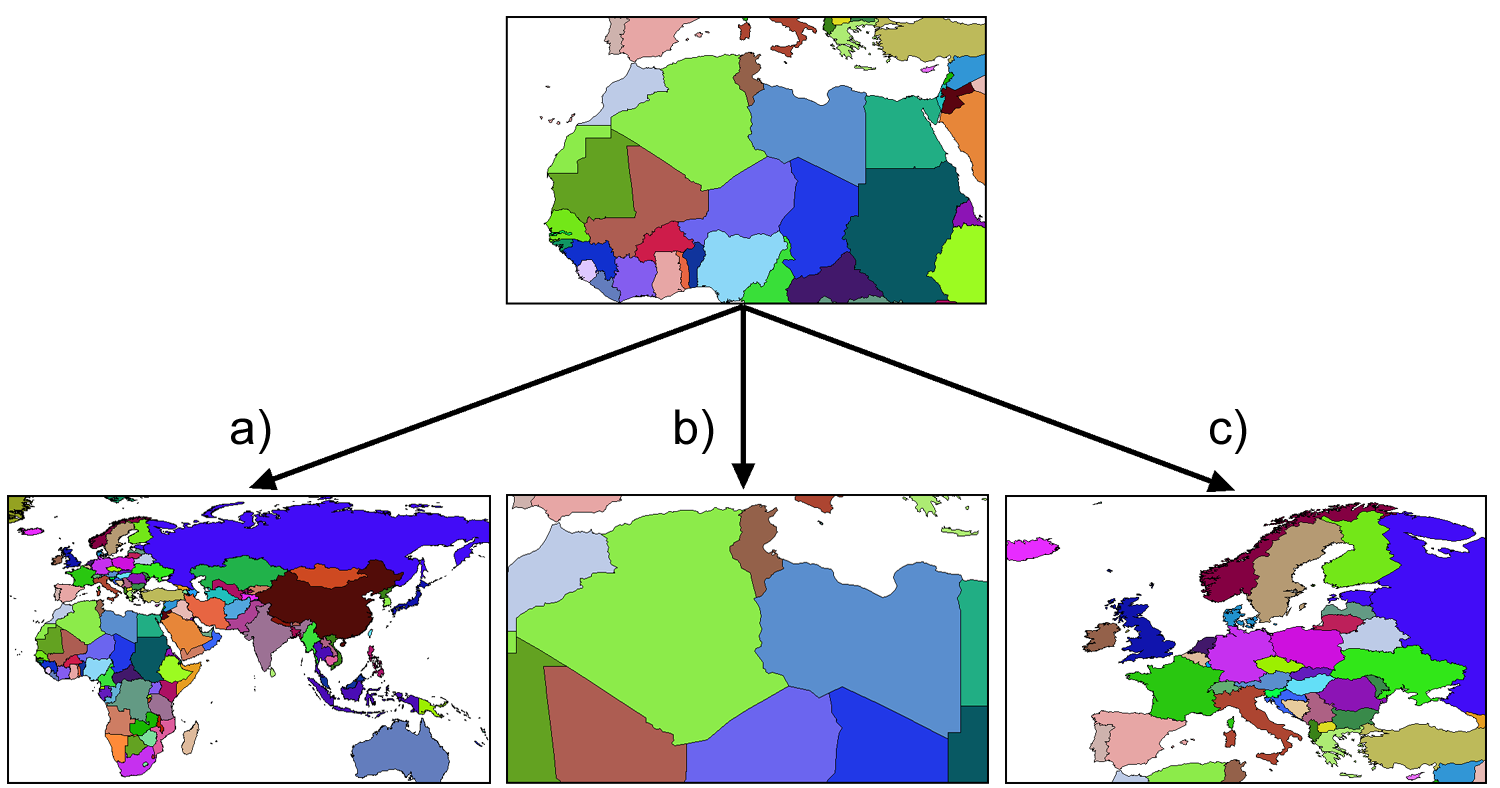
\includegraphics[width=.99\textwidth]{Software/Navigation_tools.png}

\caption{\small Navigation tools that are common in a desktop GIS. a) zoom out, b) zoom in, and c) pan}
\label{Fig:Navigation_tools} 
\end{figure}

The most remarkable feature of geographical data visualization in GIS is that, unlike what happens with a classic printed map where its characteristics cannot be changed, the user can select \emph{what} he/she sees and \emph{how} he/she sees it. Geographical data is \textbf{independent of the information needed to visualize it} and, therefore, it can be represented in different ways. This is true even for data that has an inherent visual nature, such as images, since even in that case the rendering can be adjusted and modified by the user.

Although in the most common case the canvas is bidimensional, certain GIS are also capable of \textbf{three-dimensional rendering}. In this case, navigation tools are more complex and they allow for adjusting perspective, vision angles or vertical exaggeration, among other parameters.

\subsection{Analysis}

Analysis is a fundamental functionality of GIS since its origins. Others, such as visualization, although we cannot imagine GIS without them nowadays, were very limited in the early days. Analysis, however, has always been at the core of GIS.

The current trend in GIS is to consider analysis capabilities as \textbf{modular tools} that are run on a base platform which includes the data input and output capabilities, along with the visualization component. Analysis tools are independent, but they can be used together to create more complex analyses.

Analysis tools might be completely independent of the visualization component or be linked to it. In the first case, the analysis is performed on a set of layers and parameters without any interaction with the map while in the second case, the user might interact with the view to define how the analysis is performed (for instance, selecting a coordinate or a region in the canvas which will then be used as a parameter for the analysis tool).

The result of an analysis tool in GIS can be geographical (a new layer) or not (a simple value, such as the one resulting from some statistical analysis of the input data).

Analysis tools can be organized into \textbf{workflows} which help\textbf{automate} analysis routines. Also, the analysis functionality of desktop GIS can usually be used from \emph{scripting languages}, which allow definition of more complex models and data flows. This is one of the main strengths of current GIS tools, since it provides the user more power and flexibility.

\subsection{Editing}

The geographical data with which we work in GIS are not static. Information contained in a layer \textbf{might have to be changed or corrected}, and the functionality that allows the user to do that is important if we want the GIS tool to be versatile. Without them, geographical data lose part of their potential, and that is the reason why most desktop GIS tools implement editing capabilities to some extent.

This capabilities can be used to \textbf{create new layers} or to \textbf{update existing ones}. The following are some editing tasks that can be performed with GIS:

\begin{itemize}
\item Editing the geometries of a vector layer feature.
\item Editing the attribute values of a vector layer feature, including editing the list of attributes of the layer, adding or removing them.
\item Adding new features to a vector layer or removing existing ones.
\item Editing cell values in a raster layer.
\end{itemize}

Tools used to edit geometries inherit a large part of their design from CAD software. In certain cases, they are extended with new functionalities, as happens in the case of editing geographical data with topology (CAD software does not consider topology).


\subsection{Map design}

Most desktop GIS are capable of producing cartographic documents which can later be printed and used as a classic paper map. These documents are composed in the GIS from the data, and use the same functionality that it is used for the on-screen rendering (symbology, etc.).

Along with that, other tools allow the user to \textbf{design and compose the map}, and to \emph{adjust its elements} (rendered layers, legend, title, etc.), and are inspired by those found in design software. 

Some desktop GIS include elements to \emph{automate cartographic production}, such as templates or tools to generate map series (Figure \ref{Fig:Map_series}).

\begin{figure}[!hbt]
\centering
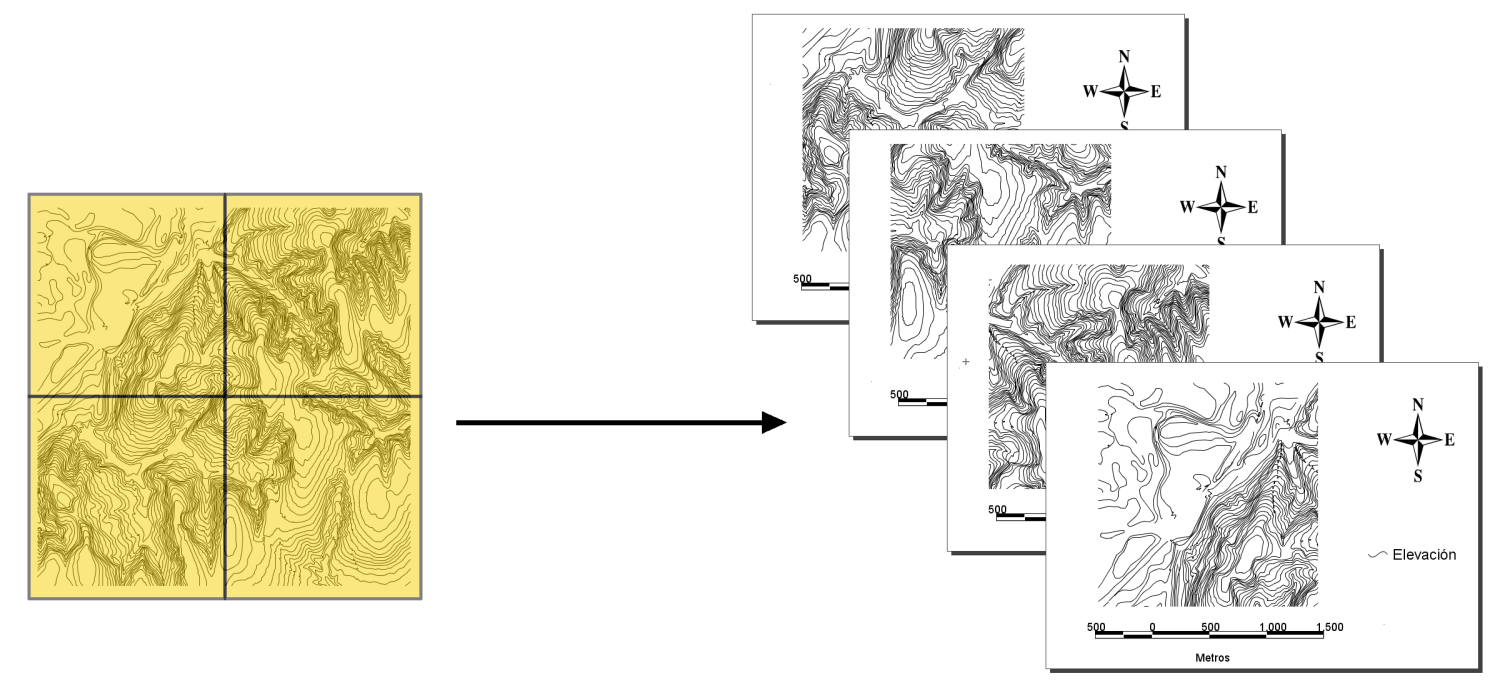
\includegraphics[width=\textwidth]{Software/Map_series.png}
\caption{\small Automated creation of map series in a GIS.}
\label{Fig:Map_series} 
\end{figure}

This is possible thanks to the \textbf{separation between geographical data and the design of the cartographic document}, similar to what we noted for the case of visualization.


\section{Web mapping. Clients and servers}

One of the most relevant advances in the history of GIS is the advent of \textbf{Web mapping}. Web mapping technologies are used to incorporate GIS elements as part of websites, with internet browsers being then the base platform on which GIS functionality is executed. These technologies include not just the elements run on the browser, and have been key in shaping and developing others such as \textbf{remote data services}, which are used not only by Web Mapping applications but also by desktop GIS.

The concepts of \emph{server} and \emph{client} are fundamental in this context. Let's discuss them in a bit more detail.

A \textbf{server} is the element that provides (serves) a given content through the network. In our GIS context, this content means basically geographical data. The \textbf{client} is the element that requests the data, receives it and works with it. 

A web browser is a client, since it makes a request to get the content of a website and shows it to the user. When we enter a web address in the address bar of a web browser, we provide the information needed to establish the connection between the server and the client and to transfer the data from one to the other.

Let's see how that works. Suppose that we want to visit the following website:

\begin{center}
\small\texttt{http://victorolaya.com/writing}
\end{center}

The requests is done based on the web address ---more technically, a Uniform Resource Locator (URL)---, which is a reference to a web resource that specifies its location on a computer network and a mechanism for retrieving it. We can divide it in the following parts:

\begin{itemize}
	\item \texttt{http}: The protocol to use, which defines the way client and server will communicate with each other.
	\item \texttt{victorolaya.com}: The host name. This part identifies the server machine connected to the network where the page that we want to visit is stored. It is a human-readable version of a numeric code that indicates the address.
	\item \texttt{writing}: The page we want among all the ones that the server can provide. 
\end{itemize}

The process that allows us to have that page in our web browser comprises the following steps:

\begin{enumerate}
	\item The client makes the request.
	\item The server machine is identified and the request is driven to it.
	\item The server prepares the page that has been requested and sends it back to the client (or it sends an error message in case it could not find or prepare the page).
	\item The client receives the page and renders it so the client can see it.
\end{enumerate}


Figure \ref{Fig:How_internet_works} shows a summary of this.

\begin{figure}[!hbt]   
\centering
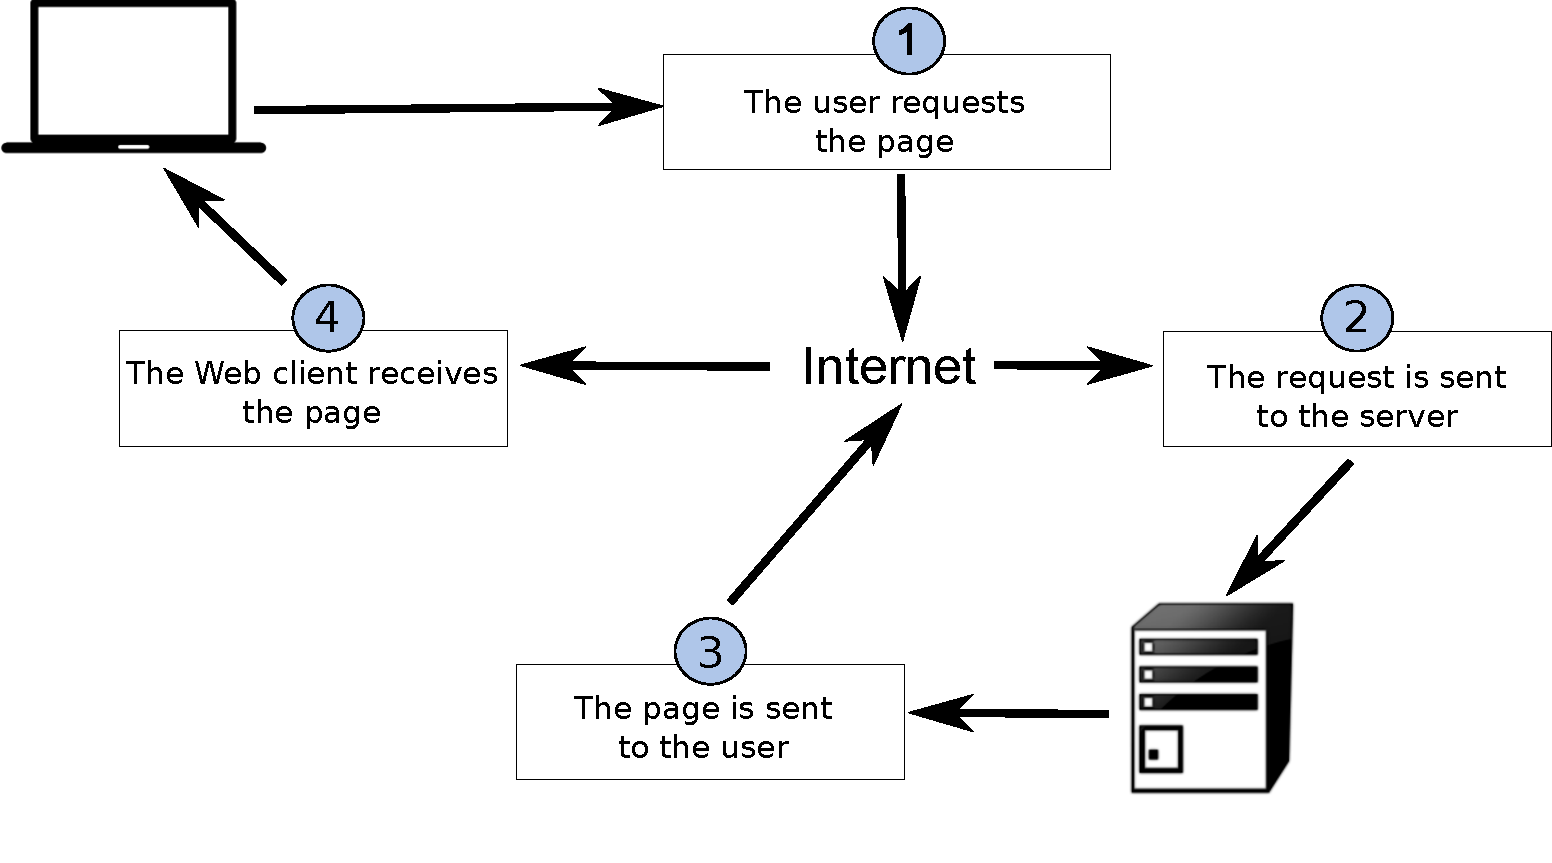
\includegraphics[width=\columnwidth]{Software/How_internet_works.pdf}
\caption{\small Client-server interaction mechanism that takes place when visiting a website.}
\label{Fig:How_internet_works} 
\end{figure}

A relation is established between clients and servers, in which an arbitrary number of clients connect themselves to a server, from which they obtain data whenever each of them makes a request. In this client-server architecture, the server has the data to be shared through a service, while clients only provide information about themselves needed to validate and perform the data sharing.

Now let's see how these ideas apply to the field of GIS.

Regarding servers, they can have four main capabilities:

\begin{itemize}
\item \textbf{Serve rendered geographical data}. Generally known as \textbf{map servers}, they provide maps. That is, images created from geographical data. If data is already an image (such as an aerial or satellite photograph), the server will just send it as it is. If data is not an image (vector layer or raster layer other than image), the server will create an image based on the geographical data. The symbology used to do this can be a default one that the server uses for all requests or it can be provided by the client in the request. 

In both cases, the client also specifies the dimensions of the requested map image that is served, and then the server prepares it.


\item \textbf{Serve the data directly}. A more flexible option is to serve the geographical data itself. The client requests the data and once it has been transmitted across the network, can use it however he/she needs. In case the data is to be visualized, the symbology has to be set in the client side, since the server is not taking care of that and provides the raw data.


\item \textbf{Serve the result of queries}. Another functionality that the server can have is to return not just the full set of geographical data, but a subset of it. The client can specify a \textbf{filter} and the server will use it to create a subset that will later be sent in the response. Also, the server can provide \textbf{descriptive values} about the data it has. The client, which might be connected to several services and obtain the values, can use those values to filter which services to use (for instance, asking them the extent of their data and then selecting only those that have data about a given study area). As we have already seen, \textbf{metadata} have a great relevance in this context, since they allow this kind of queries to be executed (and the corresponding requests to be responded to) efficiently.

\item \textbf{Serve processes}. Finally, a server can provide new data, whether geographical or not, computed from geographical data. In this case, the server provides a processing service, and it processes the data that is passed to it as part of the request. The request can contain the data itself, or a reference to it. If a reference is passed, the data might already be in the server, or it can be in another one. In this last case, the first server will become a client of the second one, will retrieve its data, process it, and send back the result to the original client (Figure \ref{Fig:Remote_data_and_services}).


\begin{figure}[!hbt]   
\centering

\includegraphics[width=0.95\textwidth]{Software/Remote_data_and_services.png}
\caption{\small Remote processing service using data from a second server.}
\label{Fig:Remote_data_and_services} 
\end{figure}

\end{itemize}

About clients, they can be divided in two classes:

\begin{itemize}

	\item \textbf{Heavy clients}. Heavy clients are independent applications that do not run on top of another one such as a web browser. They usually have a larger size since the application has to care of all the program logic.

	Heavy clients handle and use data not coming from web services, such as local data files. They are not just clients, but full-fledged applications that work even without its client part.

	Nowadays, most desktop GIS are heavy clients themselves as they have the functionality of classic GIS but can also consume web services.


	\item \textbf{Light clients}. They normally have a smaller size and their capabilities are more limited. They run on web browsers and most of the time rely on remote data from servers.

	Although originally, they focused on data visualization (adding map views to websites, with a certain degree of interactivity), they have begun to implement more advanced functionalities such as analysis functionality (whether on the client side or using a processing service) or data editing.

	The term \emph{Web mapping} is used to refer to the lighter clients which focus only on rendering maps, while the term \emph{Web GIS} is used for those with more functionality, incorporating some of the tools traditionally found in desktop GIS.
\end{itemize}

\section{Some techniques related to GIS services}

Two important techniques used in the context of the client--server architecture for geographical data are \textbf{tiling} and \textbf{caching}. These techniques, whether implemented on a light client or a heavy one, allow for more responsive interfaces and reducing the amount of data sent over the network, overcoming to a certain extent the problems that a slow network might cause. Both are used mainly with map servers (servers that provide rendered images).

Tiling divides the images that the client is working with into smaller ones, forming a mosaic. By correctly managing the tiles in that mosaic, the amount of data transmitted can be reduced. When the request is sent to the server, instead of a single image, a set of them is requested. Although this does not reduce the amount of data, the tiled structure will allow a more flexible and optimized handling of data once a new image is needed, as will soon be explained.

Caching is a technique frequently used not just for web SIG, but as a general tool in the context of the internet. Web browsers store previous responses from web servers, such as web pages and images, in a so-called \emph{cache}. When data that was previously requested is requested again, it can be taken from the cache instead of from the corresponding server, which is usually faster and more efficient.

Combining tiling and caching increasing responsiveness and results in an optimized data management. Let's see how that works, using the example shown in figure \ref{Fig:Tiling}.

\begin{figure}[!hbt]   
\centering
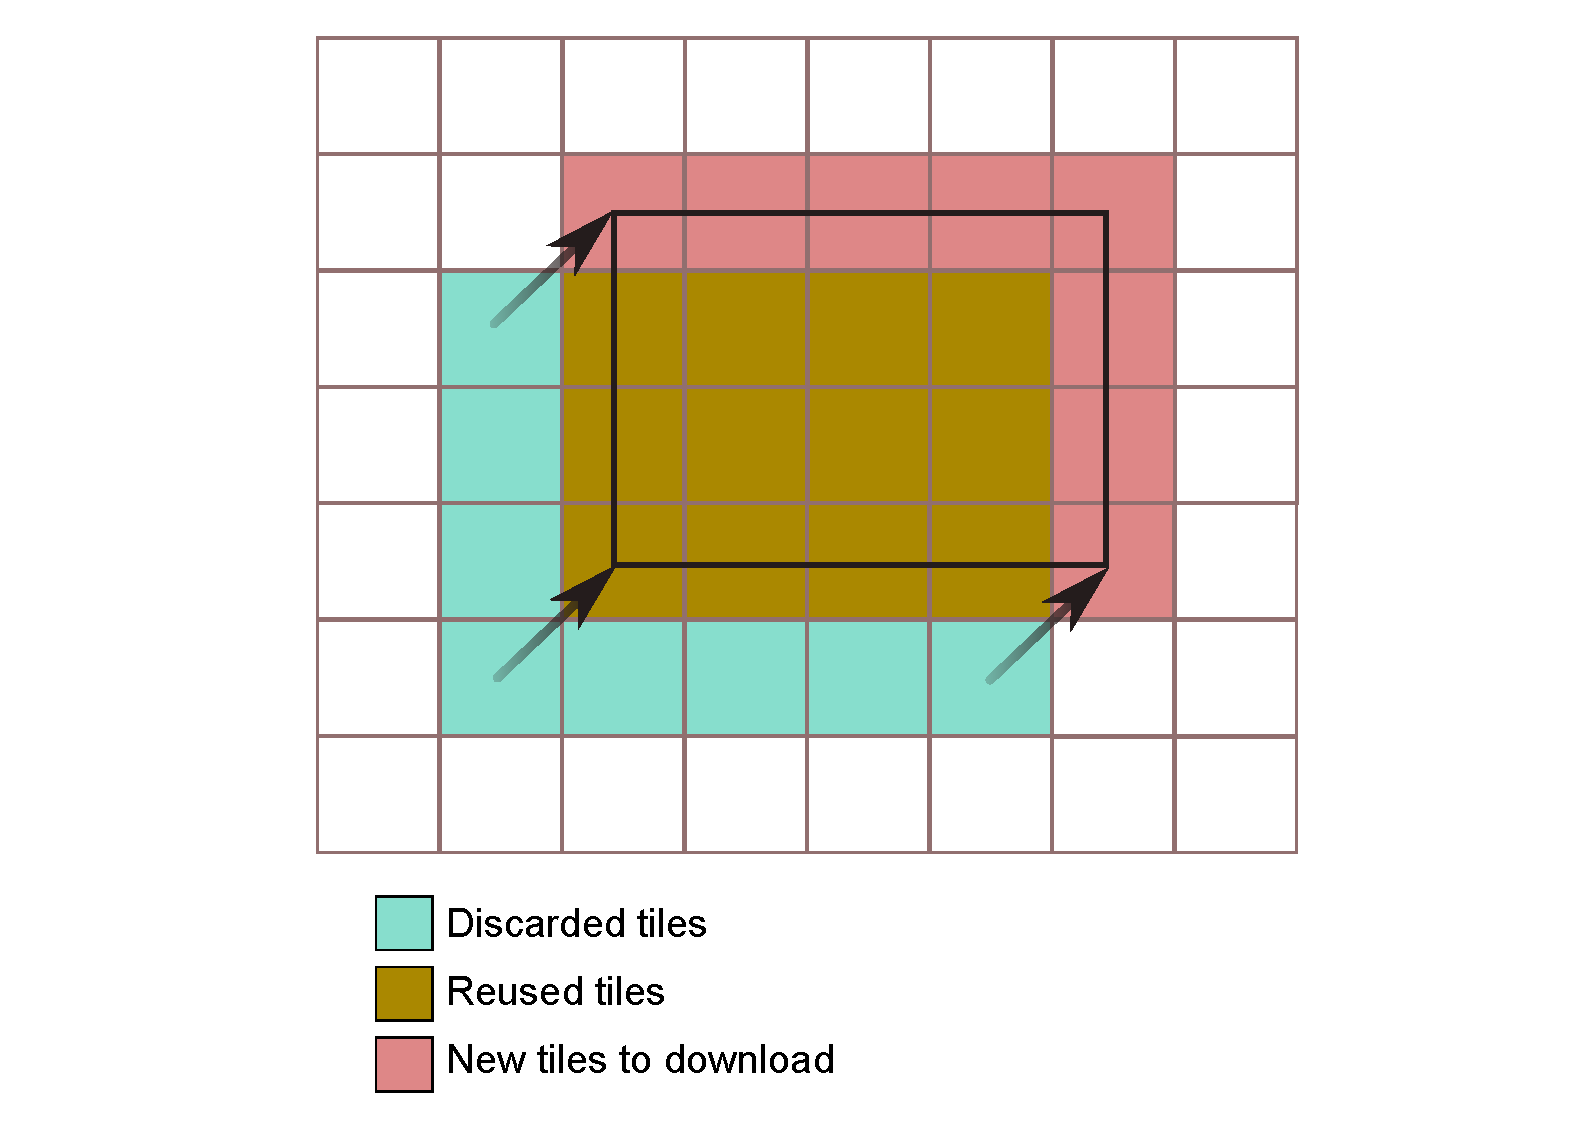
\includegraphics[width=\textwidth]{Software/Tiling.pdf}
\caption{\small Combination of tiling and caching techniques to optimize data handling in a web GIS application.}
\label{Fig:Tiling} 
\end{figure}

Initially, the application displays an area that cover 20 elements or tiles. All those tiles have already been downloaded from the server, and stored in the application cache, which means that using them again does not require making a new request to the server. Without caching and tiling, when the application user changes the area to be displayed as shown in the figure, a whole image has to be requested, with exactly the same size as the image to be rendered in the screen. However, if tiling and caching are applied, we just have the whole new image to be painted divided in 20 parts, and, since some of them are stored from a previous request, we just have to request a small number of them (8 in this case, corresponding to the areas not covered by the previous image). The amount of data that is requested to the server and transmitted over the network is much smaller.

Caching can also be implemented on the server side. We have seen that map servers provide already rendered images based on some data. Rendering that data can be time consuming and, if it has to be done for each request, that would mean a lot of computing cost for the server. Instead, images are pre-rendered at different scales so when a client request is received by the server, it just has to crop the pre-rendered image instead of producing the response image from the base data.

A recent technique that is gaining popularity is \emph{vector tiling}. Using the same approach as in the case of the tiling we have just seen (that is, cutting the data in pieces), vector layers are divided and only the required data are sent to the client.

This allows the client to request and use vector layers and be responsive at the same time. Without vector tiling, this would be impossible for large layers. The advantage in this case is that the symbology can be defined by the client. Also, the user experience is improved, since for instance, transitions become more fluent when changing the map scale, due to the scalability of vector data.




\section{Standards}

To ensure the the client-server system works correctly, it is important to define how the communication between servers and clients takes place. Some \textbf{normalization} is needed, and there must be common and well-defined elements implemented by both the client and the server. This \emph{lingua franca} that allows clients and servers to communicate is what we call a \textbf{standard}.

In an ideal situation, a complete \textbf{interoperability} would exist independent of formats and applications used. Clients and servers would be able to connect with each other, regardless of their own characteristics. Standards are the element that allows that to happen, because they define a common framework in which clients and servers communicate. As long as a client or a server follows the standard, it will be able to communicate with all others that do it as well. Standards provide \textbf{technological homogeneity}.


Interoperability means that any element of the client-server system can be replaced with another one, and the interaction between all parts of the system will not  be affected. A client or server might have different functionalities, but regardless of its origin (its manufacturer), it will be able to interact with the other elements, if all implement the same standard.

A standard is considered as such when it is used by a group or community, which accepts it to define the characteristics of a product or service within it. Standards can be established by public acceptance and custom (\emph{de facto} standards) or they might have legal recognition and be proposed by some official organization (\emph{de iure} standards).

A standard is \textbf{open} if \textbf{its definition is available} to everyone who wants to know more about it and use it for any activity related to it.

The following are some of the fundamental principles that open standards are based on:

\begin{itemize}
	\item \textbf{Availability}. Open standards are available to anyone, to read and to use.
	\item \textbf{Maximize end-user choice}. Open standards create a fair, competitive market, and do not lock users in the closed environment of a given vendor. 
	\item \textbf{No royalty}. Implementing a standard is free and has no cost, unlike the case of a patent.
	\item \textbf{No discrimination}. Open standards and the organizations behind them do not favor any implementer of the standard over the rest of them.
	\item \textbf{Extension or creation of subsets}. Standards can be extended with additional elements or reduced to less-detailed subsets.
\end{itemize}

To know the impact that a standard has in the context of GIS, let's take a look at figure \ref{Fig:Non_interoperable}, which represents a non-interoperable architecture that does not use standards.

\begin{figure}[!hbt]   
\centering
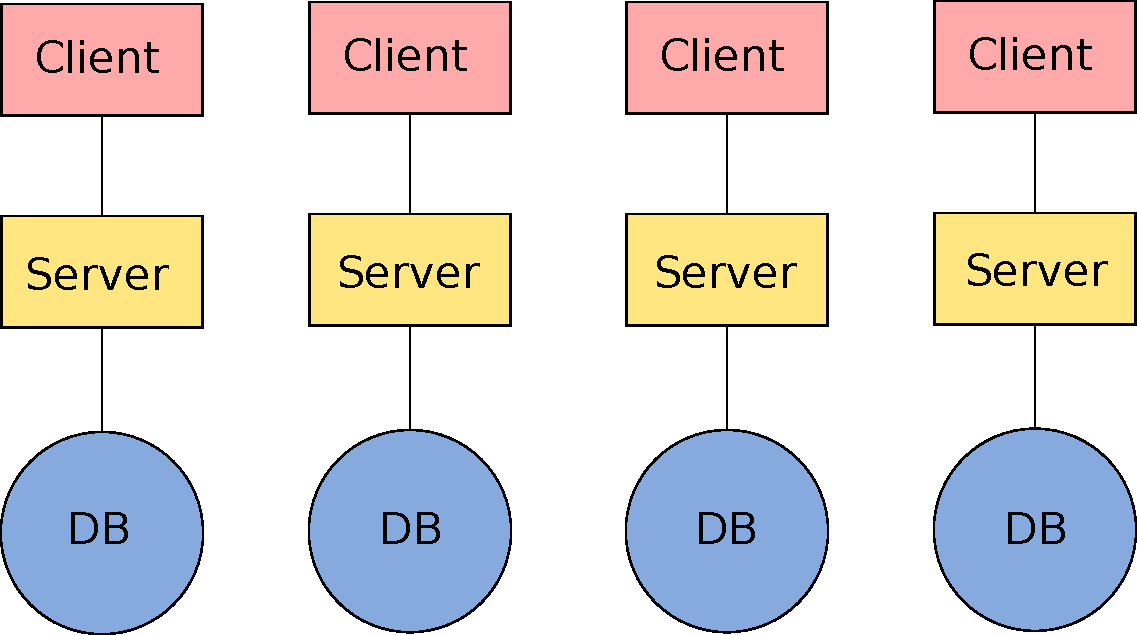
\includegraphics[width=.7\columnwidth]{Software/Non_interoperable.pdf}
\caption{\small Non-interoperable architecture.}
\label{Fig:Non_interoperable} 
\end{figure}

Data stored in each database are available only by using one client, the one corresponding to the server that serves those data. The remaining data are not available for that client. Each client-server-database group is an independent island, technologically isolated from the rest of them.

Disadvantages of a non-interoperable architecture like that include the following:

\begin{itemize}
\item \textbf{Waste of resources}. Each service must manage its own data. That is complex and has higher costs than sharing data with other compatible services.
\item \textbf{Need to know multiple clients}. Since we need a different client for each service, the user must be familiar with all of them. Being capable of using just one client is not enough to use all the available data, since that client can only access a small part of all that data..
\item \textbf{Combining data is not possible}. Two datasets that are available through two different services cannot be used in the same client, as it cannot communicate with the corresponding servers.
\item \textbf{Combining functionalities is not possible}. If data is only available to a given client, the functionality in another one (which might not be implemented in the first) cannot be used on that data. When working with that data, the user's possibilities are limited to what the corresponding client can do.
\end{itemize}

Now let's take a look at a fully interoperable architecture based on open standards, as seen in figure \ref{Fig:Interoperable}.

\begin{figure}[!hbt]   
\centering
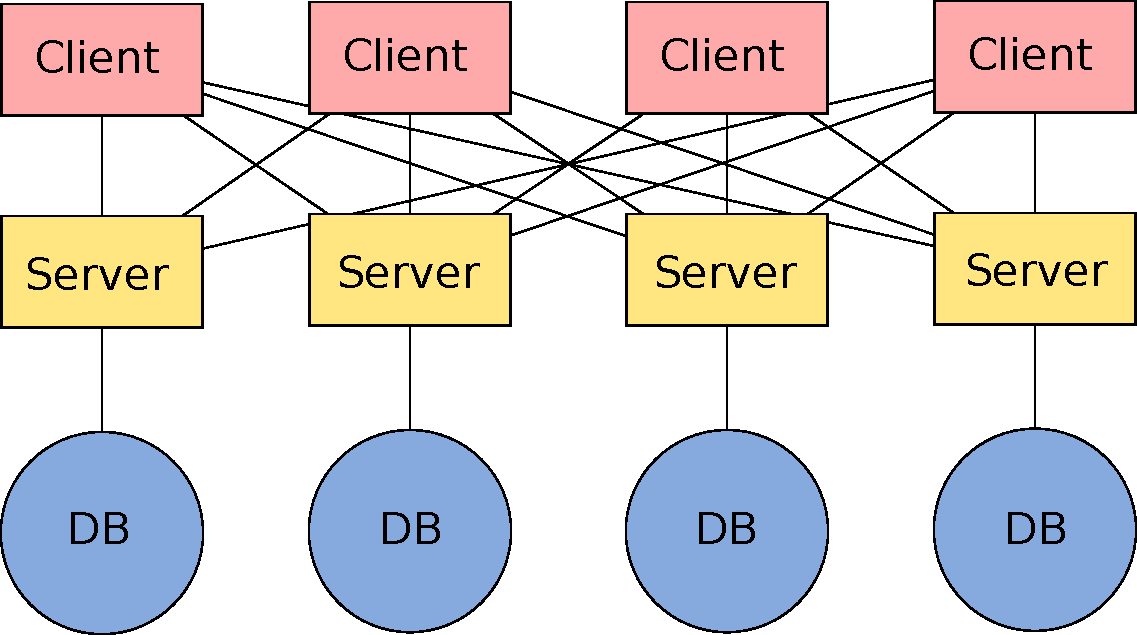
\includegraphics[width=.7\columnwidth]{Software/Interoperable.pdf}
\caption{\small Interoperable architecture.}
\label{Fig:Interoperable} 
\end{figure}

In this case, there is a server that manages and offers the services for each database, but all clients can access all servers, since they are based on open standards and communication is possible between any two of them.

\subsection{Relevant standards in GIS}

The most common standards for geographical information are created and promoted by the  \textbf{Open Geospatial Consortium (OGC)}. The OGC is ``an international not for profit organization committed to making quality open standards for the global geospatial community''.

Some of the most relevant OGC standards are the following ones:

\begin{itemize}
\item \textbf{WMS}. To serve maps (images)
\item \textbf{WCS}. To serve coverages (currently only raster layers).
\item \textbf{WFS}. To serve geographical features and attributes (vector layers). It can also allow editing features from the client.
\item \textbf{WPS}. To serve remote processing services.
\item \textbf{GML}. To store geographical information.
\item \textbf{CSW}. To make queries to a catalog that contains geographical data.
\end{itemize}

Each one of these standards is described in the corresponding specification, which is subject to change and improvement. Several versions exist for each of them.

Along with these standards are those made by organizations such as \textbf{ISO} o \textbf{W3C}, with a more general scope, but also important in the context of GIS. Among them, the most relevant standards are the ISO ones that define \textbf{how to store metadata} and the W3C standards related to \textbf{communication over the Internet}.

\section{Mobile GIS}

GIS on mobile platforms such as mobile phones or tablets has a clear relation with both desktop GIS and web GIS. It takes the elements from them and adds others derived from running on a mobile platform which expand their possibilities.

Mobile devices nowadays offer two main capabilities from the point of view of GIS: \textbf{wireless access to Internet} and \textbf{ability to know the position} of the device. 

Internet access can be used to obtain maps and geographical information from a given server, or to send field data acquired with the aid of the mobile device.

The position of the mobile device is usually known based on the GPS receiver that is part of most mobile phones. However, other approaches are also possible, from computing the position \textbf{based on the phone network} to using some \textbf{indoor positioning system} if it is available.

Knowing the position of the device allows the mobile GIS application to provide additional functionality. For instance, it might be used to make \textbf{field data acquisition} easier and more efficient (the coordinates of measured points do not have to be entered manually), or to provide \textbf{location-based services} (LBS).  

Some of the main groups in which these services can be grouped are listed next.

\begin{itemize}
	\item \textbf{Navigation}. Shortest path computation, route guidance, etc.
\item \textbf{Data acquisition}. Any type of data can be registered in the field, and the device associates to them its own position automatically.
\item \textbf{Information}. Business directories, travel guides, etc.
\item \textbf{Advertising}. Location-based advertisements, promotions for nearby shops, etc.
\item \textbf{Tracking}. Of both people and products, along predefined routes or arbitrary ones.
\item \textbf{Management}. Of infrastructures, installations or fleets.
\end{itemize}

When running in a mobile platform, a GIS has additional information about the context it is running on (position, direction of movement, speed, illumination, etc.), that it can use to provide more functionality than a desktop or web GIS running on a non-mobile platform.

\pagestyle{empty}

\chapter{Bases de datos}

\pagestyle{fancy}

Las bases de datos son un elemento fundamental en el entorno inform�tico hoy en d�a y tienen aplicaci�n en la pr�ctica totalidad de campos. Concebidas con un prop�sito general, son de utilidad para toda disciplina o �rea de aplicaci�n en la que exista una necesidad de gestionar datos, tanto m�s cuanto m�s voluminosos sean estos. En el �mbito particular de los SIG, los datos son cada d�a m�s voluminosos, debido no solo a una mayor cantidad de informaci�n, sino tambi�n a una mayor precisi�n en esta, la cual implica un mayor volumen de datos. Adem�s, presentan otra serie de caracter�sticas (uso m�ltiple, necesidad de acceso eficiente para an�lisis, necesidad de indexaci�n, etc.), haciendo todas ellas que sea recomendable el uso de bases de datos y tecnolog�as espec�ficas para su manejo.


Entendemos como \emph{Base de Datos} un \textbf{conjunto de datos estructurado y almacenado de forma sistem�tica} con objeto de facilitar su posterior utilizaci�n. Los elementos clave de la base de datos son esa estructuraci�n y sistematicidad, pues son responsables de las caracter�sticas que hacen de la base de datos un enfoque superior a la hora de gestionar datos.

Las ventajas de utilizar una base de datos frente a una gesti�n no organizada de estos las encontramos tanto en los propios datos como en el uso que se hace de ellos. Algunas ventajas que afectan directamente a los datos son las siguientes:

\begin{itemize}
	\item \textbf{Mayor independencia}. Los datos son independientes de las aplicaciones que los usan, as� como de los usuarios.
	\item \textbf{Mayor disponibilidad}. Se facilita el acceso a los datos desde contextos, aplicaciones y medios distintos, haci�ndolos �tiles para un mayor n�mero de usuarios.
	\item \textbf{Mayor seguridad (protecci�n de los datos)}. Mayor facilidad de replicaci�n de datos y mejor sincronizaci�n.
	\item \textbf{Menor redundancia}. Con el consiguiente menor volumen de datos y mayor rapidez de acceso.
	\item \textbf{Mayor eficiencia en la captura, codificaci�n y entrada de datos}.
\end{itemize}

Esto tiene una consecuencia directa sobre los resultados que se obtienen de la explotaci�n de la base de datos, present�ndose al respecto ventajas como, por ejemplo:

\begin{itemize}
	\item \textbf{Mayor coherencia}. La mayor calidad de los datos que se deriva de su mejor gesti�n deriva en mayor calidad de los resultados.
	\item \textbf{Mayor eficiencia}. Facilitando el acceso a los datos y haciendo m�s sencilla su explotaci�n, la obtenci�n de resultados es m�s eficiente.
	\item \textbf{Mayor valor informativo}. Resulta m�s sencillo extraer la informaci�n que los datos contienen, ya que uno de los cometidos de la base de datos es aumentar el valor de estos como fuente de informaci�n.
\end{itemize}

Por �ltimo, los usuarios de la base de datos tambi�n obtienen ventajas al trabajar con estas, entre los que cabe citar:

\begin{itemize}
	\item \textbf{Mayor facilidad y sencillez de acceso}. El usuario de la base de datos se debe preocupar �nicamente de \emph{usar} los datos, disponiendo para ello de las herramientas adecuadas y de una estructura solida sobre la que apoyarse.
	\item \textbf{Facilidad para reutilizaci�n de datos}. Esto es, facilidad para compartir.
\end{itemize}

De forma resumida, puede decirse que la principal bondad de una base de datos es la \textbf{centralizaci�n} que supone de todos los datos con los que se trabaja en un contexto determinado, con las consecuencias que ello tiene para una \textbf{mejor gesti�n, acceso o estructuraci�n} de estos.


\section{Bases de datos relacionales}


De entre los distintos modelos existentes para plantear una base de datos, el m�s habitual, tanto dentro como fuera del �mbito de los SIG, es de las denominadas \textbf{bases de datos relacionales}. Este modelo utiliza un esquema basado en \textbf{tablas}, que resulta a la vez sencillo de comprender y f�cil de utilizar para el an�lisis y la consulta de los datos. Las tablas contienen un n�mero dado de \textbf{registros} (equivalentes a las filas en la tabla), as� como \textbf{campos} (columnas),

La tabla en s� se conoce como \textbf{relaci�n}, ya que recoge la relaci�n existente entre sus elementos, y constituye as� el eje central del modelo relacional. Las columnas representan los distintos \textbf{atributos} asociados a la entidad, mientras que las filas conforman los distintos \textbf{registros}. Una fila se forma con un conjunto de $n$ atributos, constituyendo una \textbf{tupla}.

Una base de datos contiene normalmente m�s de una tabla, ya que suelen ser muchos los tipos de datos a almacenar y resulta conveniente dividirlos en distintas tablas.  Adem�s de las relaciones que la tabla en s� implica, es necesario definir interrelaciones entre las distintas tablas, y para ello se emplean los denominados atributos \textbf{clave}. Un atributo clave es aquel que tiene valor \textbf{�nico e invariable} para cada tupla, pudiendo servir para representar a esta plenamente. Por ejemplo, en una tabla  con nombres de personas e informaci�n adicional sobre ellas, el n�mero de su DNI puede servir como atributo clave. 


Cuando trabajamos con datos espaciales, es habitual emplear la \textbf{componente espacial como clave}, ya que esta suele ser �nica. 

Las interrelaciones entre tablas pueden ser de distintos tipos, seg�n el n�mero de entidades de una tabla con los que se relacionen las entidades de la otra. Tenemos as� relaciones de \textbf{uno a muchos}, de \textbf{uno a uno} o de \textbf{muchos a muchos}. Por ejemplo, en una tabla con entidades que representan personas y otra con entidades que representan ciudades, si establecemos una interrelaci�n \emph{vive en}, se tratar� de una interrelaci�n de uno a muchos, ya que en una ciudad pueden habitar varias personas.



\section{Sistemas gestores de bases de datos}

Junto con las bases de datos, el elemento fundamental para el aprovechamiento de estas son los \textbf{Sistemas Gestores de Bases de Datos} (SGDB o DBMS, del ingl�s \emph{DataBase Management System}). Estos sistemas representan un \textbf{elemento intermedio entre los propios datos y los programas} que van a hacer uso de ellos, facilitando las operaciones a realizar sobre aquellos. Los programas tales como un SIG no acceden directamente a la base de datos, sino que lo hacen \textbf{a trav�s de un SGBD}.


Algunas caracter�sticas que ha de tener un SGBD son las siguientes:

\begin{itemize}
	\item \textbf{Acceso transparente a los datos}. El SGBD debe crear una abstracci�n de los datos que haga el trabajo con estos m�s sencillo, ocultando aspectos internos que no sean relevantes para dicho trabajo.
	
	Procedimientos como las \textbf{consultas} se realizan a trav�s del SGBD, que es quien se encarga de interpretar dichas consultas, aplicarlas sobre la base de datos y devolver el resultado correspondiente. El SIG no accede a los datos, sino que se comunica con el SGBD y deja en manos de este el proceso de consulta en s�.
	\item \textbf{Protecci�n de los datos}. Si la base de datos almacena informaci�n sensible, el SGBD debe \textbf{controlar el acceso} a esta, restringiendo el acceso cuando corresponda (por ejemplo, estableciendo distintos permisos de acceso para distintos tipos de usuarios) e implementando los mecanismos de protecci�n necesarios.
	\item \textbf{Eficiencia}. El SGBD debe ser capaz de gestionar de forma fluida \textbf{grandes vol�menes de datos o de operaciones} (por ejemplo, muchos usuarios accediendo simult�neamente), de modo que d� una respuesta r�pida a las peticiones de los usuarios de la base de datos.
	\item \textbf{Gesti�n de transacciones}. Las operaciones sobre la base de datos tales como la adici�n o borrado de un registro se realizan mediante transacciones. El SGBD ha de encargarse de gestionarlas de manera eficiente y segura para que todos los usuarios de la base de datos puedan hacer su trabajo de forma transparente. Se denomina \textbf{transaccional} al SGBD capaz de garantizar la integridad de los datos, no permitiendo que las transacciones puedan quedar en un estado intermedio. 

\end{itemize}

En este sentido, resulta de especial importancia la existencia de \textbf{lenguajes de consulta}, que son los que una aplicaci�n utilizar� para comunicarse con el SGBD y expresar las operaciones que desea realizar con los datos de la base de datos. El lenguaje de consulta mas extendido es \textbf{SQL} (Standard Query Language)

\subsection{Bases de datos espaciales}

Todo cuanto hemos visto en los puntos anteriores constituye el conjunto de ideas fundamentales sobre las que se asienta la creaci�n y uso de bases de datos de cualquier �ndole. La inclusi�n de datos espaciales en este esquema no es en absoluto obvia, y presenta una complejidad adicional que requiere de nuevos planteamientos. Para que una base de datos pueda considerarse espacial, debe adaptarse y a�adir elementos adicionales. 

En primer lugar, el dato espacial debe poder \textbf{almacenarse de forma nativa} en la base de datos. Esto quiere decir que una geometr�a debe poder almacenarse asociada a una entidad en una tabla, del mismo modo que sucede con otros tipos de datos tales como valores num�ricos o cadenas de texto. El dato no solo debe poder almacenarse, sino tambi�n \textbf{entenderse} por parte del SGBD, para as� comprender su naturaleza espacial y poder responder a peticiones relativas a esta por parte del usuario. Esto se denomina \textbf{almacenamiento transparente}, frente al almacenamiento \textbf{opaco}, en el cual la base de datos es capaz de recoger cualquier tipo de valor, pero sin ser capaz de entender su naturaleza y utilizarlo.

Aunque existen planteamientos para almacenar datos r�ster en bases de datos, \textbf{las bases de datos espaciales trabajan principalmente con datos vectoriales} y est�n mejor adaptadas a estos. Las geometr�as del dato vectorial se incluyen, como ya se ha dicho, dentro de los valores de un registro de la tabla (que se corresponde con una entidad en el modelo de datos vectoriales). Por su parte, la componente tem�tica del dato espacial puede almacenarse sin problema en la base de datos, sin necesidad de ning�n tipo de adaptaci�n.

Cuando la base de datos est� preparada para almacenar y trabajar con los datos espaciales, es necesario \textbf{adaptar el lenguaje de consulta}. A las operaciones habituales que un SGBD es capaz de realizar en funci�n de los datos, se a�aden otras que utilizan las propiedades espaciales del dato espacial. Se tiene as� un \textbf{lenguaje de consulta espacial}, que permite consultas con componente espacial.


\section{Consultas}


Entendemos por consulta una operaci�n en la cual \emph{preguntamos} a los datos geogr�ficos alg�n tipo de cuesti�n simple, generalmente basada en conceptos formales sencillos. Este tipo de an�lisis, aunque no implica el uso de conceptos anal�ticos complejos, es uno de los elementos clave de los SIG, pues es parte b�sica del empleo diario de estos.

Aunque las consultas no son algo exclusivo de las bases de datos, es mediante el concurso de estas que adquieren toda su potencia y permite efectuar gran parte de las operaciones habituales de un SIG.

En el contexto espacial, una consulta representa un uso similar al que damos a un mapa cl�sico, cuando en base a este respondemos a preguntas como \emph{�qu� hay en la localizaci�n X?} o \emph{�qu� r�os pasan por la provincia Y?} No obstante, no debemos olvidar que los datos espaciales tienen dos componentes: una espacial y otra tem�tica. Preguntas como las anteriores hacen referencia a la componente espacial, pero igualmente pueden efectuarse consultas que se apliquen sobre la parte tem�tica. Y m�s a�n, pueden efectuarse consultas conjuntas que interroguen a los datos geogr�ficos acerca de los atributos espaciales y tem�ticos que estos contienen.


Un ejemplo muy sencillo de consulta es lo que conocemos en un SIG como \textbf{selecci�n}. De todos los registros de la tabla de datos, aquellos que cumplen el criterio indicado se marcan como seleccionados, y posteriormente pueden utilizarse �nicamente estos como base de otro an�lisis, o simplemente el usuario puede ver cu�les han sido los seleccionados para as� obtener la respuesta a su consulta. La figura \ref{Fig:Seleccion} muestra un ejemplo t�pico de esto, en el que el usuario define un �rea rectangular y se seleccionan las entidades que cumplen la condici�n de intersecar con �l. Los criterios de selecci�n pueden ser sencillos como este, o m�s elaborados y complejos.

\begin{figure}[!hbt]   
\centering
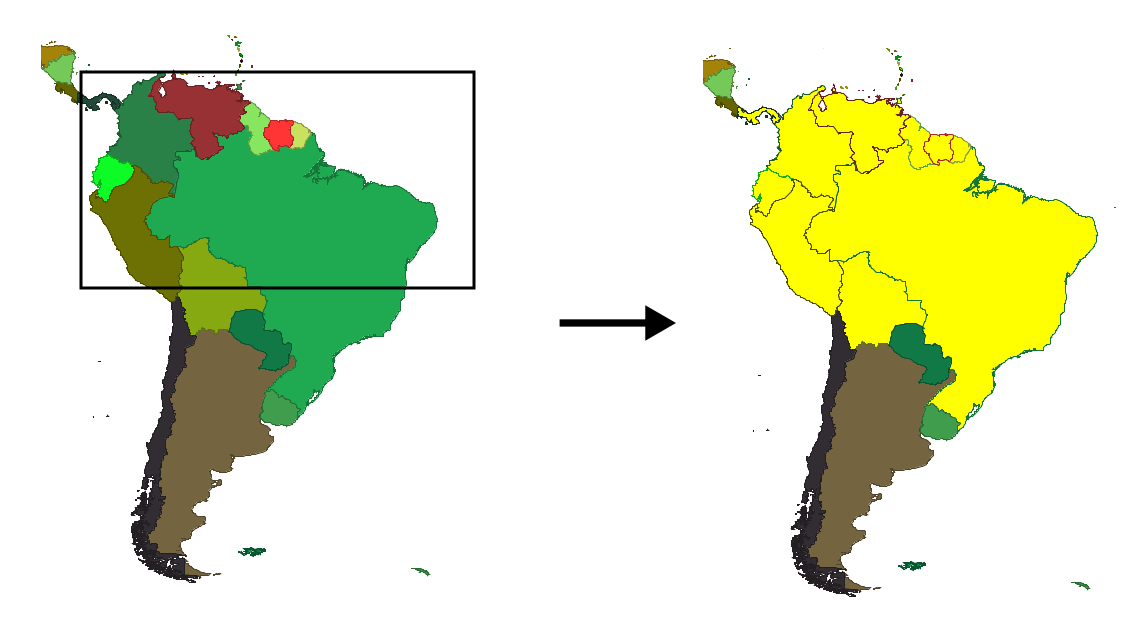
\includegraphics[width=\textwidth]{Bases_datos/Seleccion_rectangulo.png}
\caption{\small Una consulta sencilla mediante la definici�n gr�fica de un rect�ngulo. Todas las entidades dentro de este son el resultado de la consulta y quedan seleccionadas en el SIG.}
\label{Fig:Seleccion} 
\end{figure}


Una consulta nos vale tambi�n para extraer informaci�n de una base de datos de acuerdo a nuestras necesidades, y para crear posteriormente y a partir de dicha informaci�n una nueva capa. Esta operaci�n es �til cuando la base de datos de la que disponemos es muy voluminosa y solo resulta de inter�s para nuestro trabajo una parte de ella. Puede tratarse de una parte en el sentido espacial (la base de datos contiene datos a nivel mundial y se quiere trabajar a nivel estatal), en el sentido tem�tico (la base de datos contiene mucha informaci�n de cada entidad y solo interesan algunos campos), o en una combinaci�n de ambas. Para extraer dicha parte y trabajar �nicamente con ella, utilizaremos una consulta.

Veamos algunos ejemplos de consultas. Sea  una capa con los distintos pa�ses del mundo y una serie de valores econ�micos y sociales asociados a cada uno de ellos. Consideremos las siguientes preguntas:

\begin{itemize}
 \item �Qu� pa�ses tienen un Producto Interior Bruto mayor que el de Espa�a?
\item �Qu� pa�ses han experimentado un crecimiento econ�mico en el �ltimo a�o?
\item �Cu�ntos pa�ses tienen m�s de 200 millones de habitantes? 
\end{itemize}

En todos estos casos estamos haciendo referencia a pa�ses, los cuales, como sabemos, estar�n asociados a elementos geom�tricos que definan sus propiedades espaciales, es decir, a una componente espacial. Esta componente es la que permite que, adem�s de poder plantear las consultas anteriores, podamos representar cada pa�s en la pantalla y visualizarlo, o saber cu�les de ellos se encuentran en el hemisferio norte (esta ser�a una consulta espacial, de las que m�s adelante en este mismo cap�tulo veremos).

Sin embargo, cuando realizamos consultas como las tres anteriores, no acudimos para nada a la componente espacial. Consultas como estas podr�an resolverse si en lugar de una capa dentro de un SIG tuvi�ramos, por ejemplo, un simple anuario estad�stico lleno de tablas con datos correspondientes a cada pa�s. 

Las consultas pueden incluir varios criterios en una sola pregunta. Por ejemplo:

\begin{itemize}
 \item �Qu� pa�ses de la zona euro tienen m�s de 40 millones de habitantes?
\item �En qu� pa�ses de habla inglesa aument� la poblaci�n durante el �ltimo a�o?
\end{itemize}

Para expresar esas consultas se han de incluir elementos de la denominada \textbf{l�gica booleana}. Esta implica el uso de \textbf{operadores l�gicos}, mediante los cuales se reescribir�an las consultas anteriores de la siguiente manera:

\begin{itemize}
 \item �Qu� pa�ses tienen como moneda el euro \emph{y} a la vez tienen m�s de 40 millones de habitantes?
\item �Que pa�ses hablan ingl�s \emph{y} sufrieron un aumento de poblaci�n durante el �ltimo a�o?
\end{itemize}

Los lenguajes de consulta que se emplean para transmitir estas operaciones a un SGBD, permiten el uso de tales operadores para formular consultas.

Si el SGBD es de tipo espacial y \emph{entiende} que algunas de las columnas de una tabla contiene informaci�n espacial (es decir, que cada entidad no solo tiene informaci�n tem�tica), pueden plantearse consultas que hacen uso de esta, tales como las siguientes.

\begin{itemize}
\item �Qu� pa�ses comparten frontera con Alemania?
\item �Cu�ntos pa�ses se encuentran completamente en el hemisferio sur?
\item �Qu� pa�ses est�n a menos de 2000 km de Espa�a?
\end{itemize}

Para dar respuesta a esas cuestiones, basta analizar la componente espacial y no necesitamos para nada los datos con los que hemos trabajado anteriormente. Son consultas puramente espaciales. Aunque estas consultas ampl�an lo que ya conocemos, en realidad no abren ninguna nueva v�a de estudio de los datos geogr�ficos. Son consultas a las que podr�amos responder utilizando un mero mapa impreso, sin aprovechar el hecho de que dentro de un SIG las componentes espacial y tem�tica se hallan �ntimamente vinculadas. La verdadera potencia de las consultas espaciales la encontramos en la combinaci�n de estas consultas sobre la componente espacial y las que vimos anteriormente sobre la componente tem�tica. As�, se pueden plantear, por ejemplo, cuestiones como:

\begin{itemize}
 \item �Qu� pa�ses del hemisferio norte tiene una densidad de poblaci�n mayor que la de Per�?
\item �Cu�ntos pa�ses con m�s de 10 millones de habitantes se encuentran a menos de 1000 km de la frontera de Rusia?
\end{itemize}

Estas consultas incorporan elementos que hacen necesario acudir a la tabla de atributos, y otros que requieren analizar la componente espacial, estudiando las relaciones espaciales y topol�gicas de las geometr�as asociadas. 

Las consultas pueden incluir \textbf{varias capas}. Por ejemplo, si ademas de la capa de pa�ses disponemos de una capa de r�os del mundo, podr�amos responder a la pregunta \emph{�qu� pa�ses atraviesa el Nilo?}


Igualmente, las uniones entre tablas que hemos visto para el caso de la componente tem�tica pueden establecerse mediante un criterio espacial. Se tiene as� una \textbf{uni�n espacial}.

Un ejemplo muy sencillo de uni�n espacial es el que encontramos si combinamos la capa de pa�ses del mundo que venimos utilizando con una capa de ciudades del mundo. Podemos unir a la tabla de esta segunda capa todos los valores que caracterizan al pa�s al que pertenece cada ciudad. Si existe un campo com�n entre ambas tablas de atributos (por ejemplo, el nombre del pa�s), esto servir�a para efectuar esta uni�n. No obstante, esto no es necesario, ya que existe otro elemento com�n que no se encuentra almacenado dentro de la tabla, pero que puede tomarse de la componente espacial: toda ciudad debe estar situada dentro de los l�mites del pa�s al que pertenece. Esto sirve para establecer la relaci�n entre las tablas, y cada ciudad debe relacionarse con aquella entidad dentro de cuya geometr�a se encuentre el punto que la representa.



\subsection{�ndices espaciales}


Si realizamos una consulta a una base de datos, el resultado es un subconjunto de esta con los elementos que cumplen el criterio expresado en la consulta. Si se implementa de forma \emph{directa} dicha consulta, esta operaci�n implica comprobar todos los elementos de la base de datos y ver cu�les son los que cumplen con el citado criterio. Teniendo en cuenta que una base de datos puede tener un gran tama�o, esta forma de proceder no es la �ptima.

Los �ndices nos permiten \emph{alcanzar} los elementos que constituyen la respuesta a nuestra consulta, haci�ndolo de la forma m�s r�pida y llegando hasta ellos sin tener que pasar por todos los restantes.

Un ejemplo f�cil de entender es el de una gu�a telef�nica en la que los nombre est�n ordenados alfab�ticamente. Gracias a ese orden y a que se conoce el alfabeto, se puede buscar r�pidamente un nombre sin necesidad de leer todos ellos.

Al utilizar una base de datos, si no disponemos de un �ndice deberemos recorrer toda ella para dar respuesta a nuestras consultas. No sabemos \emph{d�nde} buscar las respuestas a nuestras consultas, del mismo modo que si no supi�ramos que carece de sentido buscar en la letra F el n�mero telef�nico del se�or P�rez.

Ademas de �ndices para datos de tipo num�rico o texto, en los que resulta obvio establecer un orden natural, en el �mbito de los SIG tienen importancia los denominados \textbf{�ndices espaciales}. Aunque sus fundamentos te�ricos son distintos, el concepto es similar al de �ndices de bases de datos no espaciales: elementos que permiten \textbf{optimizar las consultas mediante una correcta estructuraci�n} de los datos, en particular en este caso de su componente espacial.

Puede entenderse la idea de un �ndice espacial mediante un sencillo ejemplo de c�mo empleamos ideas parecidas a los �ndices espaciales de forma natural cuando tratamos de resolver una consulta espacial sin la ayuda de un SIG. Supongamos que tenemos nuestro mapa de pa�ses del mundo y queremos averiguar qu� pa�ses tienen su frontera a menos de 3000 kil�metros de la frontera de Espa�a. �C�mo operar�amos de manera natural para dar respuesta a esta consulta?

La soluci�n m�s inmediata es medir la distancia entre Espa�a y todos los pa�ses restantes, y despu�s tomar aquellos que hayan arrojado un resultado de distancia menor a 3000. La operaci�n dar�a el resultado esperado, pero implicar�a un gran n�mero de mediciones, y no ser�a una forma �ptima de operar. M�s probable es que no efectuemos mediciones con los pa�ses de Am�rica, pues un conocimiento b�sico de geograf�a basta para saber que todos ellos se encuentran a m�s de 3000 kil�metros. No sabemos exactamente a qu� distancia se encuentran, pero sabemos que no van a cumplir el criterio establecido en la consulta. 

Ese conocimiento b�sico de geograf�a que tenemos es en realidad una especie de �ndice espacial. No sirve para saber las distancias exactas ni resolver la consulta por completo, pero sirve para \textbf{dar una aproximaci�n y facilitar el trabajo}. Descartamos un buen numero de pa�ses de forma casi inmediata, y luego solo realizamos las operaciones costosas (la medici�n) con un subconjunto del total. 

De modo similar, los �ndices espaciales nos permiten obtener resultados en un �rea concreta sin necesidad de analizar todo el espacio ocupado por el total de los datos. Gracias a ello, hacen las consultas mas efectivas y permiten trabajar con grandes vol�menes de datos.

Los �ndices espaciales se almacenan junto con los datos a los que hacen referencia, bien en ficheros adicionales o dentro de la propia base de datos, en caso de utilizarse una. Los SGBD espaciales tienen \textbf{capacidades para calcular estos �ndices espaciales} y almacenarlos en la base de datos, recurriendo a ellos cuando se realiza una consulta que requiera su uso.


\pagestyle{empty}

\chapter{An�lisis espacial. Fundamentos}
\label{Analisis}


\pagestyle{fancy}

El an�lisis espacial es una de las tareas fundamentales sin las cuales el concepto de SIG no alcanza su verdadero significado. 

El an�lisis espacial es el \textbf{estudio cuantitativo de aquellos fen�menos que se manifiestan en el espacio}. Ello indica una importancia clave de la posici�n, la superficie, la distancia y la interacci�n a trav�s del propio espacio. 

Ejemplos de an�lisis que realizamos con cartograf�a fuera de un SIG son el buscar en un mapa d�nde se sit�a el pico m�s alto, ver la elevaci�n concreta a la que se encuentra un elemento dado tal como una poblaci�n, o planificar una jornada tur�stica viendo qu� lugares de inter�s podemos visitar o c�mo llegar desde uno a otro de estos lugares haci�ndolo por las mejores carreteras o de la forma m�s r�pida. Estas actividades habituales son ejemplos de an�lisis geogr�ficos que podemos igualmente realizar dentro de un SIG.

Mediante el an�lisis podemos generar nuevos datos que pueden ser \textbf{nuevas capas de datos geogr�ficos, tablas de datos, valores escalares} o \textbf{vectores}.

En ocasiones, los resultados expresan \textbf{la misma variable} que el dato de partida (por ejemplo, el c�lculo de una media), y en otros las variables de entrada y salida son \textbf{distintas} (por ejemplo, si a partir de una capa de elevaciones calculamos una de pendientes).

Asimismo, todo an�lisis espacial parte de un conjunto de datos espaciales, pudiendo estos ser \textbf{de un �nico tipo, o de varios distintos} que se combinan en un procedimiento concreto. Por ejemplo, en el caso de calcular la localizaci�n del punto m�s alto, el resultado es una sencilla coordenada, y tan solo se utiliza la variable elevaci�n. En el caso de la altura media de una ciudad, se utilizan dos entradas: por un lado, la elevaci�n, y por otro, el emplazamiento de la ciudad. Aunque un mapa cl�sico contiene toda esa informaci�n en una �nica hoja, en realidad son dos elementos distintos combinados a la hora de representarlos. En t�rminos m�s acordes con un SIG, podemos decir que tenemos dos capas distintas que utilizamos como entradas.

El an�lisis dentro un SIG nos permite tanto formular como responder a cuestiones. Estas cuestiones pueden ser:

\begin{itemize}
 \item Relativas a posici�n y extensi�n
\item Relativas a la forma y distribuci�n
\item Relativas a la asociaci�n espacial
\item Relativas a la interacci�n espacial
\item Relativas a la variaci�n espacial
\end{itemize}

Algunos ejemplos de an�lisis geogr�fico son los siguientes.

\begin{itemize}
\item \textbf{Consulta espacial}. Vimos las consultas en detalle dentro del cap�tulo dedicado a las bases de datos.

\item \textbf{An�lisis topol�gico}. Pueden plantearse consultas referidas no solo a la posici�n de los elementos geogr�ficos, sino a la \textbf{relaci�n con otros elementos}. La existencia de topolog�a puede emplearse para la realizaci�n de consultas que respondan a cuestiones como:

\subitem �C�mo llegar desde mi posici�n actual hasta una coordenada concreta por la red viaria existente?

\subitem �Qu� comunidades aut�nomas comparten l�mite con Madrid?

\item \textbf{Medici�n}. La existencia de una referencia espacial para cada uno de los elementos con los que trabajamos en el an�lisis dentro de un SIG hace que podamos \textbf{cuantificar} otra serie de par�metros tambi�n espaciales. Entre las mediciones m�s b�sicas, encontramos las distancias, �reas, per�metros o factores de forma. Mas elaboradas, encontramos otras como pendientes o indices derivados de medidas simples.


\item \textbf{Combinaci�n}. Uno de los procedimientos m�s habituales y m�s caracter�sticos dentro del uso de un SIG es la \textbf{combinaci�n o superposici�n} de varias capas de informaci�n. La propia estructura de la informaci�n geogr�fica en capas facilita notablemente estos procedimientos y convierte a los SIG en plataformas ideales para llevar a cabo an�lisis donde se combina informaci�n sobre diversas variables.



\item \textbf{Transformaciones}. Podemos englobar dentro de este grupo una amplia serie de procedimientos que modifican los elementos de entrada de diversas formas. Entre los m�s habituales, encontramos la \textbf{transformaci�n de coordenadas}, la \textbf{simplificaci�n de geometr�as}, o la \textbf{creaci�n de �reas de influencia} o la \textbf{reclasificaci�n de valores}. Estas transformaci�n pueden afectar tanto a la componente espacial como a la componente tem�tica del dato. 

\item \textbf{An�lisis de superficies}. El an�lisis de superficies es uno de los m�s potentes de cuantos encontramos en un SIG. Desde par�metros b�sicos como la \textbf{pendiente} o la \textbf{orientaci�n} hasta par�metros morfom�tricos muy espec�ficos, pasando por todas las herramientas del \textbf{an�lisis hidrol�gico}, la bater�a de operaciones disponibles es muy amplia. 

\item \textbf{Estad�stica descriptiva}. Los elementos de la estad�stica cl�sica tienen sus equivalentes en los datos espaciales, y nos permiten \textbf{calificar cuantitativamente} los datos con los que trabajamos. Se incluyen aqu� descriptores de centralidad y dispersi�n, de dependencia espacial o el estudio de patrones espaciales, entre otros muchos. Estos pueden a su vez usarse para el contraste de hip�tesis que contengan una cierta componente espacial.

Por ejemplo, estos estad�sticos nos permiten dar respuesta a cuestiones del tipo

\subitem �Es constante la media de altura a lo largo de toda la geograf�a de mi pa�s?

\subitem �Existe alguna direcci�n predominante en los movimientos de individuos de una especie o se desplazan err�ticamente?

\item \textbf{Inferencia}. Otro an�lisis estad�stico de gran importancia en los SIG es el que permite inferir comportamientos de las distintas variables y estudiar, por ejemplo, la forma en que estas van a evolucionar a lo largo del tiempo.

El establecimiento de modelos de cambio y variaci�n representa una de las herramientas m�s actuales en el campo de los SIG, y un campo en abundante desarrollo.

\item \textbf{Toma de decisiones y optimizaci�n}. La estructura de la informaci�n geogr�fica en capas dentro de un SIG, favorable como ya vimos para la superposici�n de capas, lo es igualmente para estudiar de forma combinada los efectos de distintos factores. Este estudio nos permite luego responder a cuestiones como, por ejemplo,

\subitem �Cu�l es el mejor lugar para emplazar una nueva construcci�n en funci�n de su impacto sobre el medio?

\subitem �D�nde situar un nuevo hospital para que el servicio en la comarca mejore lo m�ximo posible?

\item \textbf{Modelizaci�n}. La creaci�n de modelos espaciales dentro de un SIG es una tarea a�n pendiente de mucho desarrollo. No obstante, existe un gran n�mero de modelos en los m�s diversos campos, y la arquitectura de datos y procesos de los SIG es propicia para la implementaci�n de otros nuevos.
\end{itemize}

\section{Particularidades de los datos espaciales para su an�lisis}
\label{Analisis_espacial}


Las caracter�sticas propias de los datos espaciales dotan a estos de una \textbf{gran potencialidad} de an�lisis, al tiempo que \textbf{condicionan o limitan} otras operaciones. Algunas de estas caracter�sticas representan problemas que han de tenerse presentes en el an�lisis; otros son simplemente conceptos b�sicos que deben conocerse pero no han de implicar necesariamente una dificultad asociada.

\subsection{Escala}
\label{Escala_analisis}

A la hora de estudiar la informaci�n geogr�fica, podemos hacerlo a \textbf{distintos niveles} y, dependiendo del nivel elegido, los resultados ser�n de una u otra naturaleza. Debido a esto, adem�s de considerar la escala cartogr�fica para la representaci�n y gesti�n de datos en un SIG, es necesario considerar la \textbf{escala de an�lisis}.

La escala de an�lisis depende \textbf{del dato en s�} (precisi�n, tipo, etc.), as� como del \textbf{an�lisis que se va a realizar} con �l.

Como se muestra en la figura \ref{Fig:Escalas_formas_terreno}, si para definir las formas de relieve en un punto dado lo hacemos considerando dicho punto y los valores de elevaci�n a su alrededor, la caracterizaci�n que hagamos var�a en funci�n de la dimensi�n de esa zona alrededor (que es la que define la escala de an�lisis). Para valores peque�os de dicha zona de an�lisis, el punto analizado puede definirse como una cima, mientras que aumentando la escala de an�lisis se advierte que el punto se sit�a en el fondo de un valle.

\begin{figure}[h]   
\centering
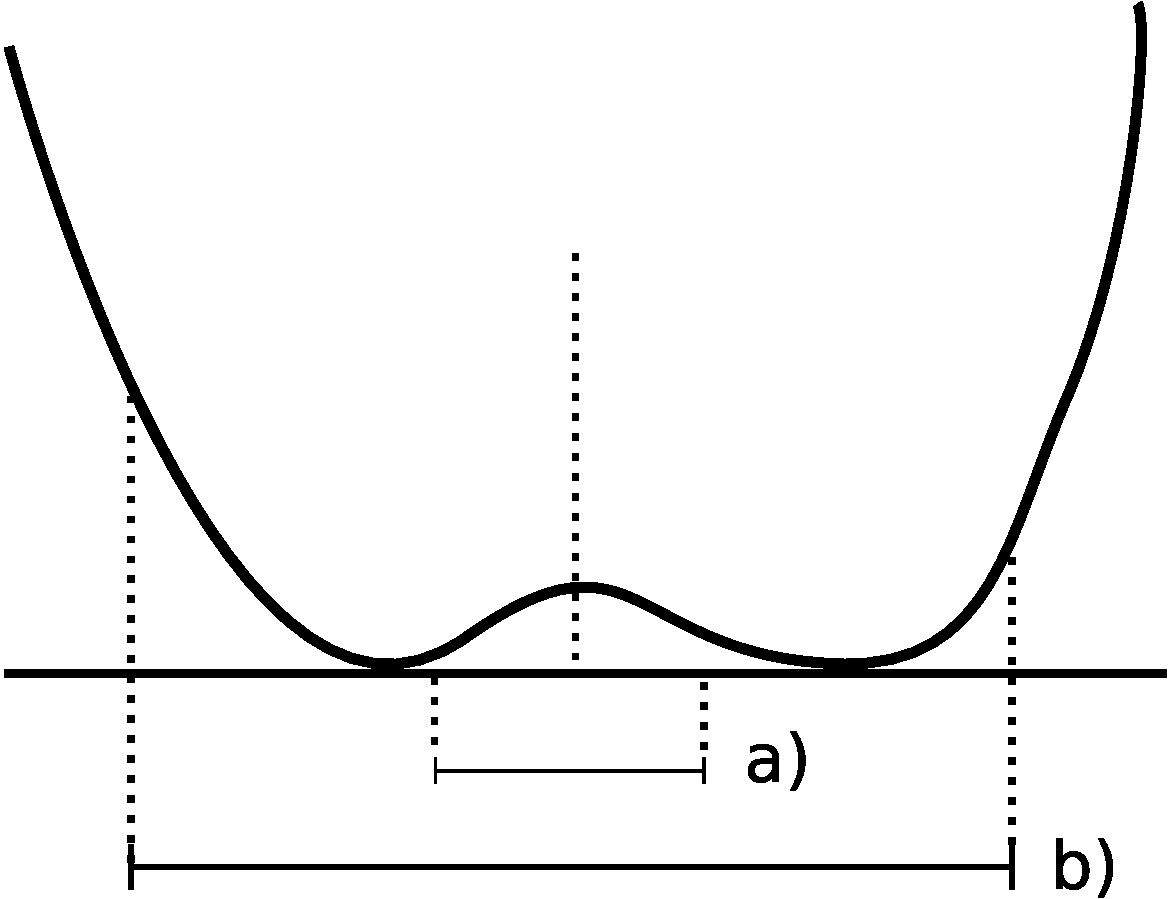
\includegraphics[width= .45\columnwidth]{Analisis/Escalas_formas_terreno.pdf}
\caption{\small Dependiendo de la escala de an�lisis, un mismo relieve puede ser caracterizado como cima (a) o fondo de valle (b)}
\label{Fig:Escalas_formas_terreno} 
\end{figure}

Por tanto, debemos observar el relieve desde la distancia correcta a la cual la informaci�n que nos proporciona es la m�s adecuada para un an�lisis dado. Adem�s de existir una escala de mayor relevancia para un an�lisis concreto,  es de inter�s el trabajar a \textbf{m�ltiples escalas} y combinar los resultados.

Otro ejemplo de c�mo la escala de an�lisis condiciona los resultados obtenidos lo encontramos en el caso de efectuar \textbf{mediciones}. Como puede verse en la figura \ref{Fig:Medida_linea_fractal}, la unidad de medida empleada provoca que se obtengan resultados distintos. 

\begin{figure}[h]   
\centering
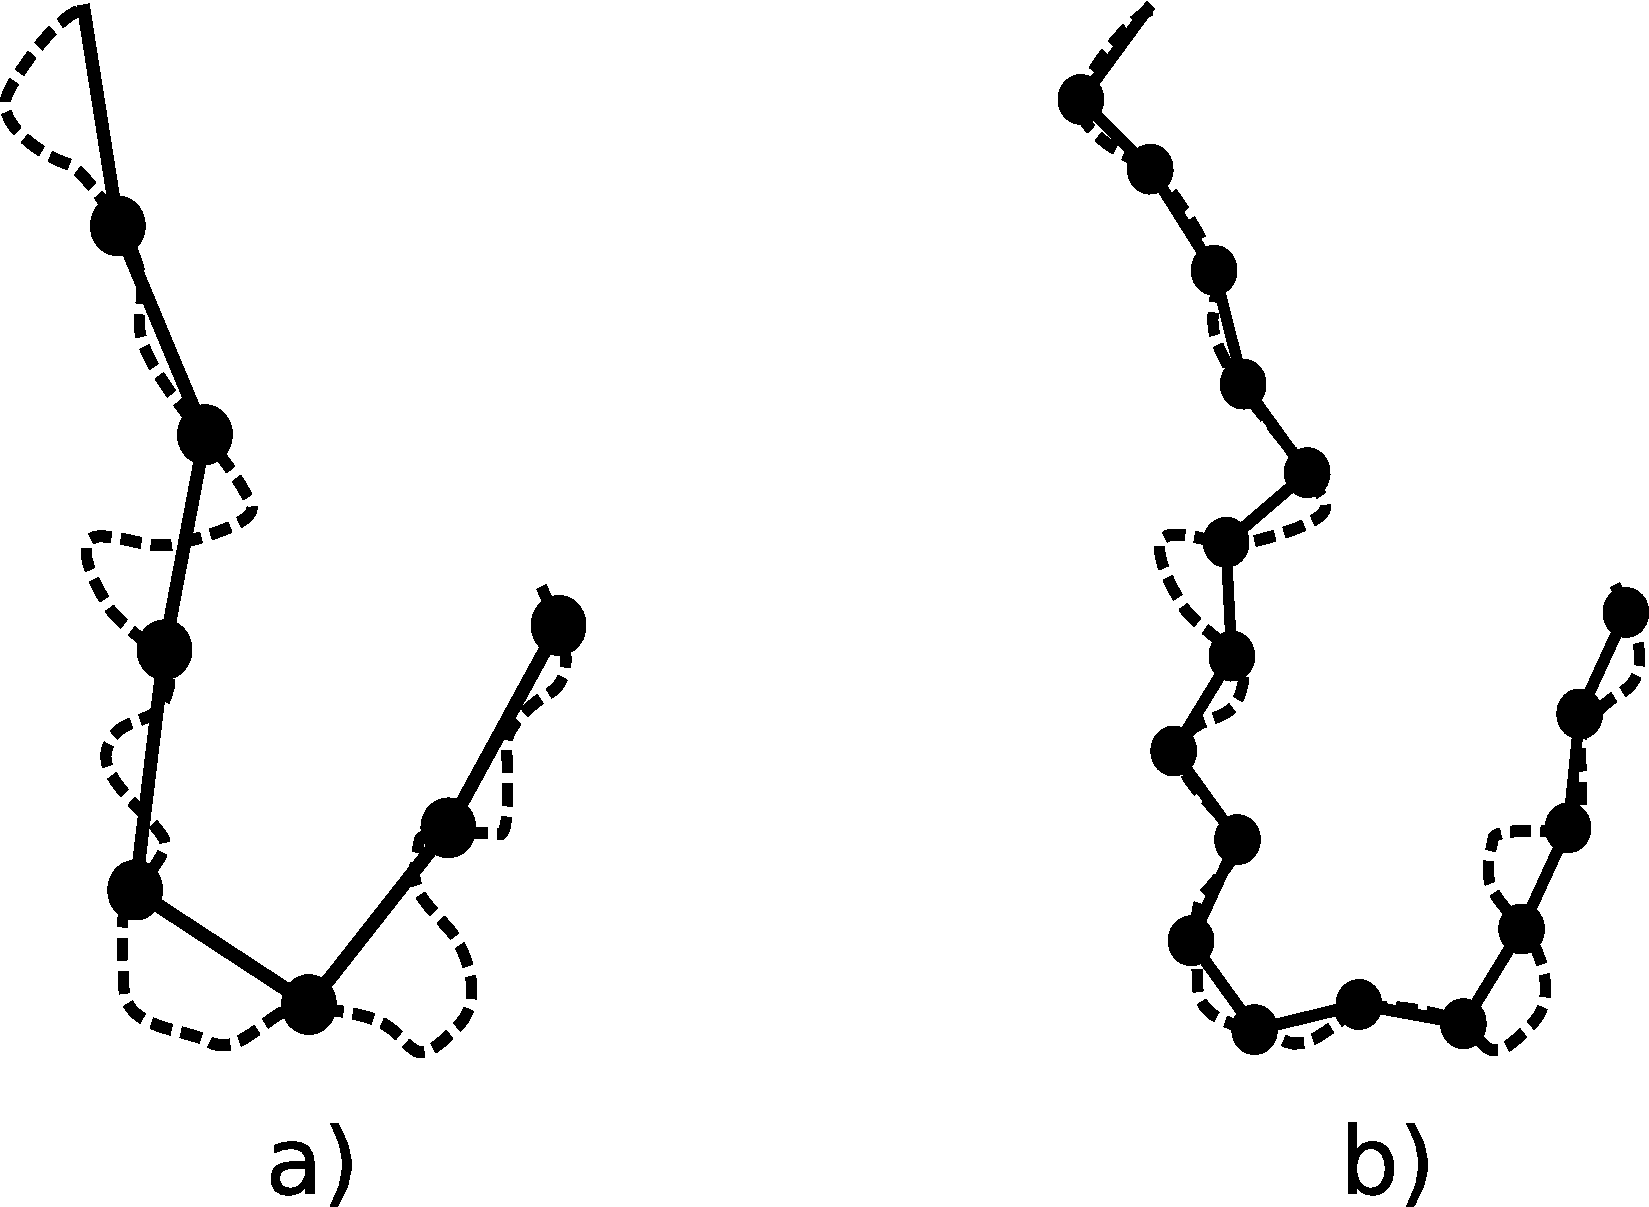
\includegraphics[width= .45\columnwidth]{Analisis/Medida_linea_fractal.pdf}
\caption{\small La unidad de medida empleada modifica el resultado obtenido.}
\label{Fig:Medida_linea_fractal} 
\end{figure}

La uni�n del valor resultante con la escala a la que se ha obtenido tiene en conjunto pleno significado, pero ese valor por s� mismo carece de dicho significado. 

El concepto de \textbf{fractal} tiene una implicaci�n directa en este hecho.

El propio \textbf{formato de almacenamiento} condiciona el efecto de la escala, ya que puede imponer l�mites. Tal es el caso cuando se trabaja con capas raster, en las que el \textbf{tama�o de celda} delimita la precisi�n que puede obtenerse en el an�lisis.

\subsection{El Problema de la Unidad de �rea Modificable}
\label{MAUP}

Muchas de las variables con las que trabajamos dentro de un SIG \textbf{no pueden medirse de forma puntual}, y por ello han de \textbf{estudiarse para un �rea dada}. Ejemplos de este tipo de variables son el porcentaje de poblaci�n en un rango de edad determinado o la densidad media de poblaci�n.

Las �reas que se definen para poder trabajar con las variables de esta �ndole son \textbf{esencialmente arbitrarias}, tales como pa�ses, regiones o distritos, que se establece sin ning�n criterio propio del an�lisis espacial. La utilizaci�n de una u otra unidad \textbf{altera los resultados} extra�dos de las variables estudiadas.

Este problema, por tener relaci�n con la elecci�n de la unidad de agregaci�n de la informaci�n, se conoce como \emph{Problema de la Unidad de �rea Modificable}(PUAM).


Un problema particular relacionado con el PUAM es la denominada \textbf{falacia ecol�gica}, que consiste en asumir que los valores calculados para una unidad de �rea pueden aplicarse a los individuos de la poblaci�n existente en dicha �rea. S�lo en el caso de que exista una completa homogeneidad para la variable analizada, lo cual raramente sucede, la anterior suposici�n ser�a cierta.

\subsection{Autocorrelaci�n espacial} 
\label{Autocorrelacion_espacial}

Se denomina \textbf{autocorrelaci�n espacial} a la existencia de una \textbf{correlaci�n de la variable consigo misma}, de tal modo que los valores de esta variable en un punto guardan relaci�n directa con los de esa misma variable en otros puntos cercanos. Por ejemplo, en el caso de medirse la temperatura, los puntos cerca de un foco de calor tendr�n una temperatura mayor que aquellos cerca de focos fr�os. Si estudiamos la distribuci�n de una enfermedad infecciosa, es m�s probable que los casos se encuentren agrupados, de forma que la presencia de un alto n�mero de casos implique tambi�n una alta incidencia en poblaciones cercanas.

Otra forma de expresar la autocorrelaci�n espacial es mediante la conocida como \textbf{Primera Ley Geogr�fica de Tobler}, que establece que <<todo est� relacionado con todo, pero las cosas pr�ximas entre s� est�n m�s relacionadas que las distantes>>.

La autocorrelaci�n espacial, tal y como se ha descrito antes, es \textbf{positiva}. Puede, no obstante, existir una \emph{autocorrelaci�n espacial negativa}, si los valores altos se rodean de valores bajos y viceversa.

En caso de no existir ning�n tipo de autocorrelaci�n espacial, se tiene que los datos recogidos en una serie de puntos son \textbf{independientes entre s�} y no se afectan mutuamente, sin que tenga influencia de la distancia.

La figura \ref{Fig:Autocorrelacion_espacial} muestra unas sencillas capas r�ster en las que se presentan los tres tipos de autocorrelaci�n espacial anteriores.

\begin{figure}[!hbt]   
\centering
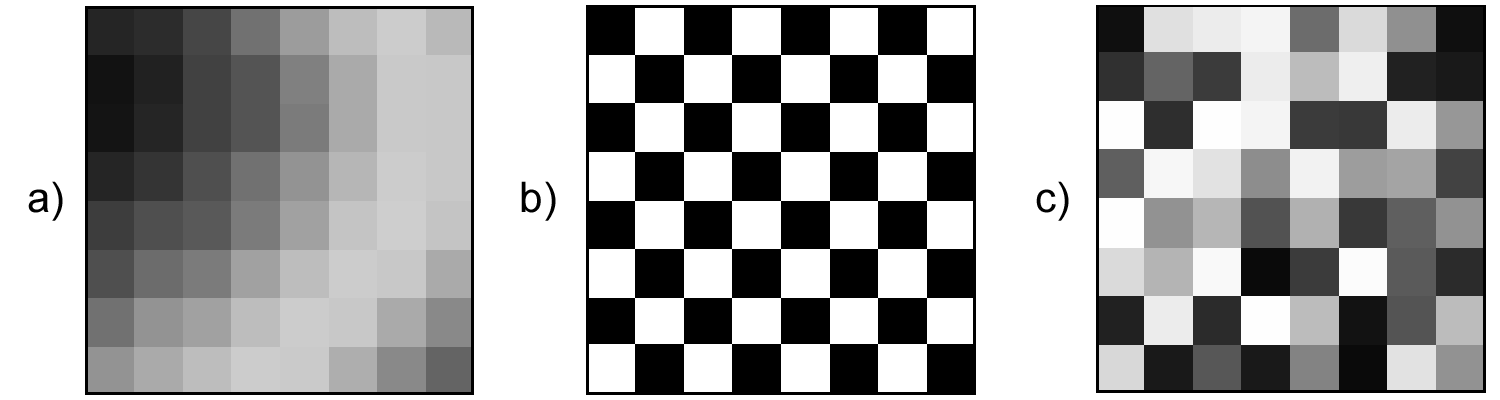
\includegraphics[width=\textwidth]{Analisis/Autocorrelacion_espacial.png}
\caption{\small a) Autocorrelaci�n espacial positiva. b) Autocorrelaci�n espacial negativa. c) Ausencia de autocorrelaci�n espacial (independencia)}
\label{Fig:Autocorrelacion_espacial} 
\end{figure}

Las consecuencias de la existencia de autocorrelaci�n espacial son numerosas y de gran importancia.

Por una parte, muchos de los an�lisis estad�sticos suponen la \textbf{independencia de la variable}. Puesto que existe una dependencia de la componente espacial, ser� necesario para obtener resultados correctos introducir dicha componente espacial como una variable m�s. 

Algo similar sucede cuando los datos presentan alguna \textbf{tendencia espacial} (los valores de una variable est�n relacionados con sus propias coordenadas geogr�ficas), ya que esto tambien invalida el supuesto de la independencia de los datos.

Existiendo autocorrelaci�n espacial, y siendo esta positiva, la \textbf{inferencia estad�stica es menos eficaz} que si se cuenta con un n�mero igual de observaciones de una variable independiente. 

La autocorrelaci�n espacial no es, no obstante, un elemento que siempre tenga consecuencias negativas. Puesto que los puntos cercanos a uno dado guardan relaci�n con este, la autocorrelaci�n puede aprovecharse para \textbf{estimar valores} en un punto cualquiera si conocemos los valores en puntos cercanos. Este es el fundamento de los \textbf{m�todos de interpolaci�n}


\subsection{Existencia de estructura}

Tanto la disposici�n de los datos como las propiedades de la variable estudiada (por ejemplo, la propia autocorrelaci�n espacial como propiedad intr�nseca) exhiben una estructura determinada. Esta estructura puede condicionar los resultados del an�lisis y tener influencia sobre estos.

Los dos principales conceptos estad�sticos que definen la estructura espacial de los datos son la \textbf{estacionaridad} y la \textbf{isotrop�a}. La estacionaridad indica que el proceso es \textbf{invariante a la traslaci�n}. Es decir, que las propiedades son constantes en el espacio y no existe tendencia alguna. La isotrop�a indica que el proceso es \textbf{invariante a la rotaci�n} y tiene lugar del mismo modo en todas direcciones. 


\subsection{Efectos de borde}
\label{EfectoBorde}

Las zonas que estudiamos dentro de todo an�lisis espacial \textbf{tienen unos l�mites establecidos}. Estos l�mites vienen definidos de forma artificial ---el l�mite de la fotograf�a a�rea de la que disponemos, por ejemplo--- o bien de forma natural ---si estudiamos un bosque junto a un pantano, el bosque encuentra su l�mite al borde de este �ltimo---. La presencia de estos bordes \textbf{distorsiona el resultado de los an�lisis}, en especial para aquellos par�metros no puntuales que requieren la definici�n de un area de estudio (densidades, etc., como ya vimos para el caso del PUAM)

En algunos casos, el efecto de borde no se manifiesta �nicamente para puntos cercanos a dicho borde, sino para \textbf{todos aquellos relacionados o conectados} con �l seg�n un determinado criterio, con independencia de su distancia a este.


\pagestyle{empty}
\chapter{Visualizaci�n y representaci�n de datos espaciales. }


\pagestyle{fancy}

Visualizar la informaci�n geogr�fica es una parte fundamental del trabajo con un SIG. Aunque algunos datos incluyen su propia manera de representarse ---por  ejemplo, las im�genes de sat�lite, las ortofotos, o las obtenidas de un servicio de mapas---, en el SIG es en general el usuario quien define la forma de representar el dato. Es decir, el usuario de SIG \textbf{toma el papel del cart�grafo}, y por tanto debe conocer los fundamentos que este utiliza para la creaci�n de mapas.

Adem�s de las herramientas y conceptos cartogr�ficos cl�sicos, los SIG incorporan elementos de la denominada \textbf{visualizaci�n cient�fica}, tales como la \textbf{interactividad} o la \textbf{representacion de datos multidimensionales}. El resultado de este nuevo planteamiento, m�s rico que el de la cartograf�a cl�sica, se conoce como \textbf{geovisualizaci�n}. 

En este cap�tulo veremos las ideas fundamentales sobre la visualizaci�n de datos, desarrollando la aplicaci�n de estas en la cartograf�a tradicional, as� como en el �mbito de la geovisualizaci�n y de los SIG.


\section{Conceptos b�sicos de visualizaci�n}

Cuando visualizamos cualquier tipo de informaci�n geogr�fica, ya sea a trav�s de un mapa cl�sico o de alg�n elemento gr�fico en la pantalla de un ordenador, estamos utilizando un \textbf{lenguaje visual} para transmitirla. Del mismo modo que al hablar empleamos un lenguaje oral y al escribir un lenguaje escrito, siempre que plasmemos la informaci�n geogr�fica en una serie de elementos visuales estaremos empleando este lenguaje visual.


El estudio de los signos de un lenguaje constituye lo que se conoce como \textbf{semiolog�a}. En el caso de los elementos del lenguaje visual, encontramos una \textbf{semiolog�a gr�fica}. Esta semiolog�a trata los signos del lenguaje visual y la gram�tica de estos, definiendo una ling��stica visual que nos ayuda a comprender c�mo una representaci�n gr�fica dada cumple su prop�sito de transmitir la informaci�n en base a la cual se crea.


\subsection{Las variables visuales}

Existen diversas propiedades de los elementos visuales que podemos emplear para trasnmitir una informaci�n, siendo m�s adecuadas unas u otras seg�n sea la circunstancia.

\begin{figure}[!hbt]
\centering
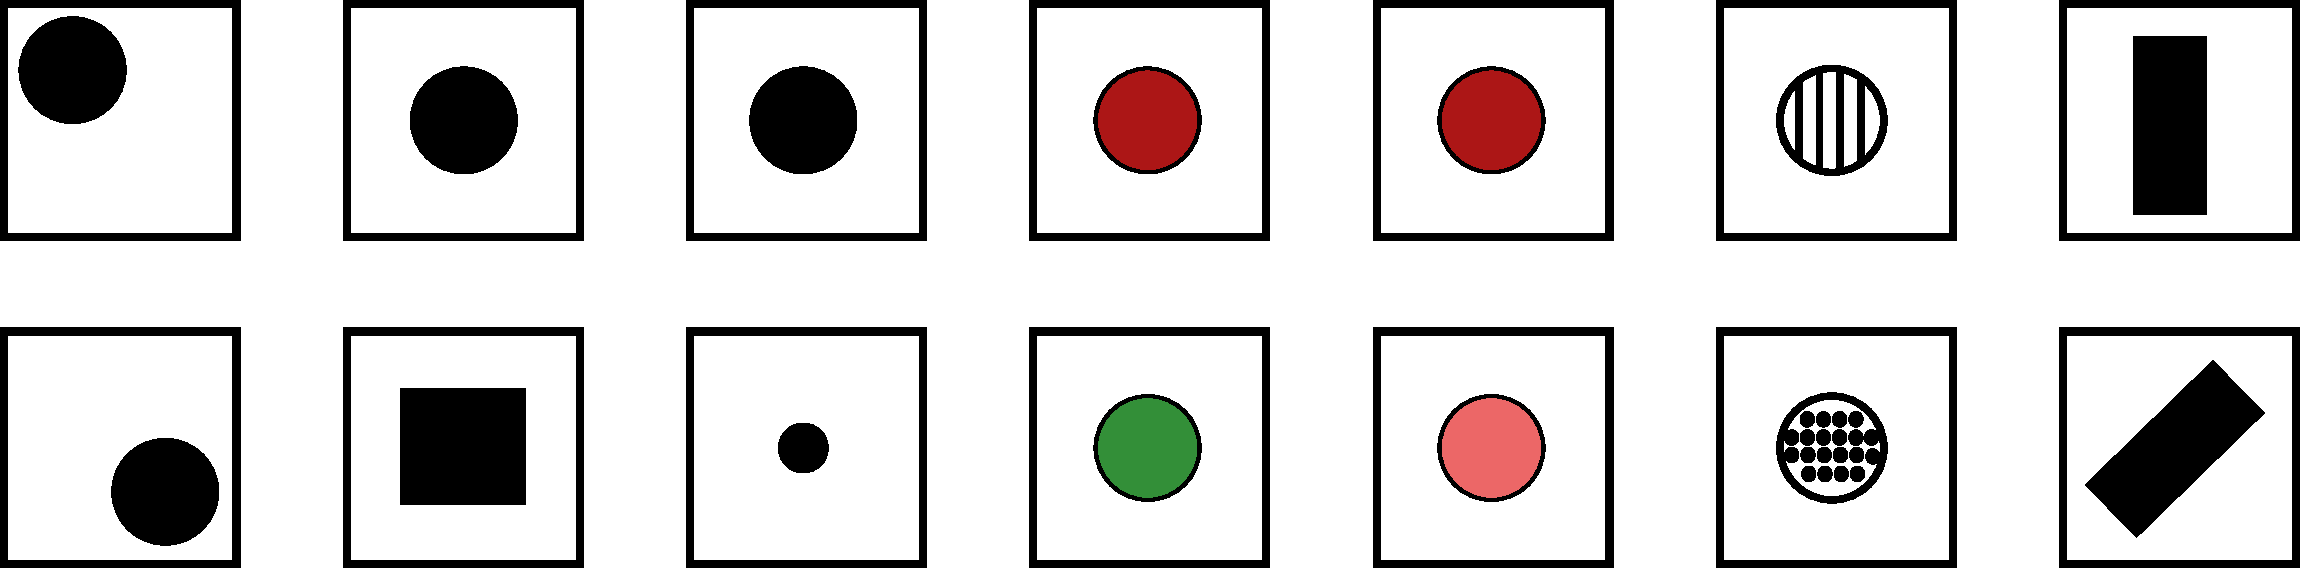
\includegraphics[width=\columnwidth]{Visualizacion/VariablesVisuales.pdf}
\caption{\small Ejemplo de uso de las distintas variables visuales. De izquierda a derecha: posici�n, forma, tama�o, tono, valor, textura, y orientaci�n}
\label{Fig:VariablesVisuales} 
\end{figure}


Estas propiedades conforman lo que se conoce como \textbf{variables visuales}, y se aplican a los elementos b�sicos de la representaci�n, que son aquellos objetos geom�tricos de que se compone esta. Las variables visuales permiten diferenciar unos de otros y asignarles unas ciertas caracter�sticas, susceptibles a su vez de ser interpretadas junto al propio significado que el objeto pueda tener. Dados dos elementos, estos pueden diferenciarse por las siguientes variables, que aparecen representadas en la figura \ref{Fig:VariablesVisuales}: Posici�n, forma, tama�o, textura, color y orientaci�n

El uso de la \textbf{posici�n} est� muy restringido en el caso de un mapa, por deber respetarse el emplazamiento real en el espacio del elemento representado, y por ello y no se emplea.

La \textbf{forma} viene definida por el per�metro exterior del objeto. La forma se aplica fundamentalmente a los s�mbolos puntuales, situando un s�mbolo de una forma dada sobre las coordenadas exactas del punto a representar. Su aplicaci�n a s�mbolos lineales es dif�cil y no se da, mientras que en el caso de aplicarse sobre s�mbolos de superficie requiere la alteraci�n de los pol�gonos representados (por ejemplo, que tracen los l�mites de pa�ses), dando lugar a una representaci�n imprecisa, al menos en lo que al contorno del pol�gono respecta. 

El \textbf{tama�o} se refiere a la dimensi�n del s�mbolo. Para el caso de s�mbolos puntuales, puede aplicarse sin m�s que hacer m�s grande o peque�o el s�mbolo en s�. En el caso de l�neas, el grosor de estas constituye la forma de aplicar la variable tama�o. No se usa en s�mbolos superficiales, salvo aplic�ndolo sobre la textura de relleno.

El tama�o \textbf{condiciona la percepci�n de otras variables visuales}, especialmente cuando se trata de tama�os peque�os. 

La \textbf{textura} hace referencia al relleno de un s�mbolo mediante alg�n patr�n. Se aplica en lineas mediante el uso de guiones y espacios en blanco que dan lugar a un patr�n de discontinuidad, aunque su uso principal es en el caso de s�mbolos de superficie.

El \textbf{color} es la m�s importante de todas las variables visuales, debido a las posibilidades que ofrece.

Dos son las componentes de un color que se utilizan como variables visuales, y que pueden entenderse como tales por si mismas: el tono y el  valor. 

El \textbf{tono} es lo que en el lenguaje com�n denominar�amos color, es decir el nombre del color, por ejemplo verde, rojo o amarillo. 

El tono puede verse \textbf{alterado por los tonos del entorno}, especialmente en s�mbolos de peque�o tama�o. Aunque es una variable para la que la percepci�n humana tiene gran sensibilidad, en los s�mbolos peque�os puede ser dif�cil de identificar y pueden producirse una falsa percepci�n si comparten espacio con otras m�s grandes de un tono distinto. 

Por su parte, el \textbf{valor} indica la claridad del color. Un tono azul puede ser m�s claro o m�s oscuro sin dejar de ser azul. Esa variaci�n que se produce es una variaci�n del valor del color. 

La capacidad de diferenciar dos s�mbolos con valor distinto var�a en funci�n del tipo de s�mbolo. As�, es mayor en el caso de s�mbolos de superficie, mientras que en el caso de s�mbolos puntuales y lineales est� relacionada con el tama�o. Si el punto es muy peque�o o la l�nea muy delgada, es m�s dif�cil apreciar el valor y, por tanto, comparar este con otro o extraer la informaci�n que mediante esa variable visual se intenta transmitir.


Por �ltimo, la \textbf{orientaci�n} se aplica sobre los s�mbolos puntuales, siempre que estos no presenten simetr�as que impidan percibir correctamente la orientaci�n. Para los s�mbolos de superficie, se aplica a trav�s de la textura, variando la orientaci�n de esta. No se aplica en el caso de l�neas.

\subsection{Las propiedades de las variables visuales}

Se distinguen 4 propiedades b�sicas que una variable visual puede presentar:

\begin{itemize}
	\item \textbf{Asociativa}. Una variable visual presenta la propiedad asociativa si al ser aplicada no aumenta ni disminuye la visibilidad de un elemento. Es decir, cuando en funci�n de esa variable visual no puede asign�rsele m�s o menos importancia a este.
	\item \textbf{Selectiva}. La propiedad selectiva la presentan aquellas variables visuales que, al ser aplicadas, generan distintas categor�as de s�mbolos.
	\item \textbf{Ordenada}. Cuando una variable visual puede emplearse para representar un orden, se dice que presenta la propiedad ordenada.
	\item \textbf{Cuantitativa}. Cuando, adem�s del orden, una variable puede mostrar cantidades o proporciones, entonces se dice que posee la propiedad cuantitativa.
\end{itemize}

En la anterior lista, las propiedades est�n organizadas seg�n los denominados \emph{niveles de organizaci�n}. La propiedad asociativa se sit�a en el nivel m�s bajo, mientras que la cuantitativa ocupa el m�s alto. El nivel de organizaci�n de las variables visuales tiene importancia a la hora de combinar varias de ellas en un s�mbolo, como veremos m�s adelante. Asimismo, el nivel de organizaci�n define qu� tipo de informaci�n podemos transmitir con una variable visual.

La figura \ref{Fig:PropiedadesVariablesVisuales} muestra diferentes representaciones de un conjunto de s�mbolos puntuales en los que en cada caso se ha utilizado �nicamente una variable visual.

\begin{figure}[!hbt]
\centering
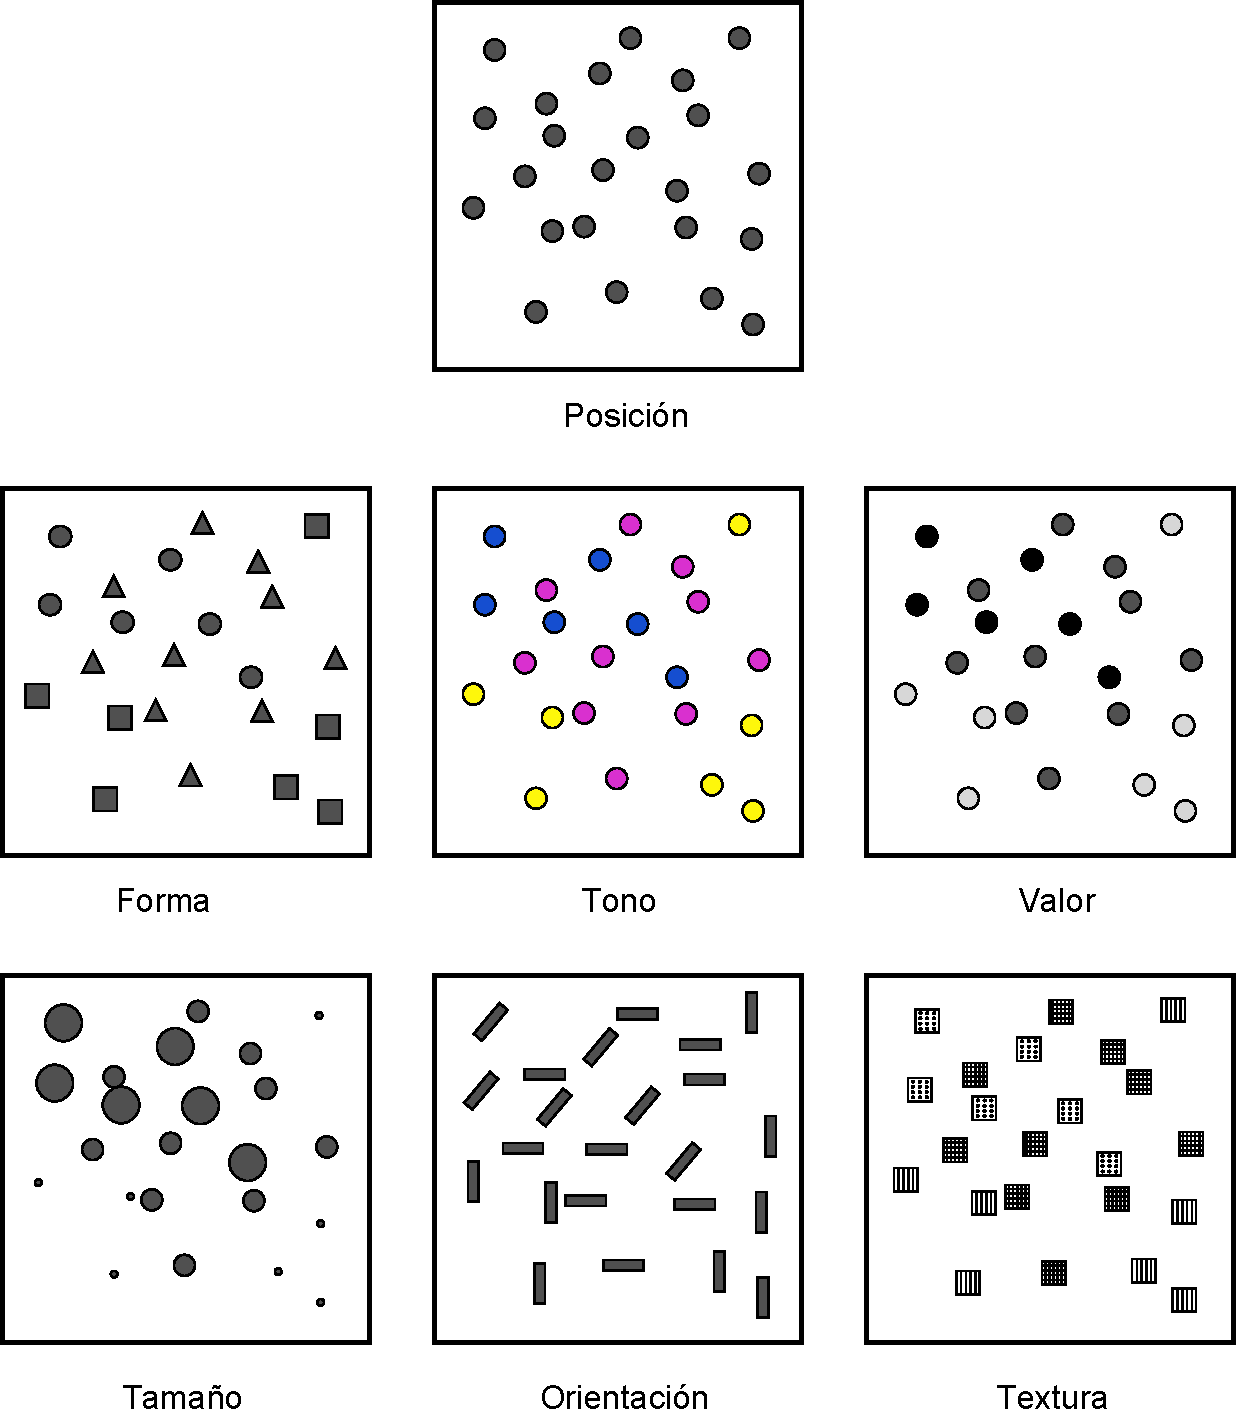
\includegraphics[width=\columnwidth]{Visualizacion/PropiedadesVariablesVisuales.pdf}
\caption{\small Representaci�n de un conjunto de s�mbolos aplicando de forma individual las distintas variables visuales.}
\label{Fig:PropiedadesVariablesVisuales} 
\end{figure}

Comenzando con la propiedad asociativa, vemos que a excepci�n del tama�o y el valor, las dem�s variables visuales no hacen que los elementos presenten una preponderancia en la imagen. No existen una orientaci�n que podamos definir como m�s importante, ni tampoco un color. Lo mismo sucede con la textura, la forma y la posici�n. 

Con el tama�o, sin embargo, resulta claro que mayor tama�o implica un papel destacado dentro de la informaci�n que transmite el mapa. De igual modo, un mayor valor (un color m�s oscuro) da sensaci�n de mayor definici�n, y centra la atenci�n de observador sobre el elemento de un modo muy superior a como lo hace un valor bajo.

Respecto a la propiedad selectiva, diremos que una variable visual la presenta si de un vistazo podemos r�pidamente seleccionar los elementos que pertenecen a un determinado grupo, identificados estos mediante dicha variable visual. El caso m�s claro de propiedad selectiva lo presenta el tono. Podemos r�pidamente quedarnos solo con los elementos amarillos o con los rojos. Aunque no de un modo tan claro, todas las restantes variables presentan igualmente esta propiedad, a excepci�n de la forma. La forma no permite que los elementos se agrupen de modo espont�neo en familias, y su validez en este sentido est� muy ligada a la complejidad de dicha forma.

La propiedad ordenada la presentan aquellas variables que permiten establecer un orden. Tan solo posici�n, textura, tama�o y valor la presentan, mientras que las dem�s carecen de ella. Por ejemplo, en la imagen correspondiente a la variable visual tono no podemos decir cu�les de los elementos situar�amos al principio y cu�les al final de una escala dada definida por esos tonos. Con el valor, sin embargo, s� que podemos, ya que esta escala ir�a de los tonos m�s claros a los m�s oscuros, y visualmente podemos sin dificultad distinguir los distintos niveles y ordenarlos.

Por �ltimo, la propiedad cuantitativa la presentan aquellas variables visuales que permiten estimar proporciones o cantidades de forma visual. Esta propiedad es exclusiva del tama�o y de la posici�n, mientras que las dem�s no la presentan. Podemos por, ejemplo ver que los c�rculos grandes en la figura correspondiente son aproximadamente el doble que los peque�os. 

En el cuadro \ref{Tabla:PropiedadesVariablesVisuales} se muestra un resumen de todo lo anterior.

\begin{table}[!hbt]
\small
\centering  \label{Tabla:PropiedadesVariablesVisuales}
\begin{tabular}{p{3.6cm}ccccccc}  
 & \rotatebox{90}{\textbf{Posici�n}} & \rotatebox{90}{\textbf{Tama�o}} & \rotatebox{90}{\textbf{Forma}} & \rotatebox{90}{\textbf{Valor}} & \rotatebox{90}{\textbf{Tono}} & \rotatebox{90}{\textbf{Textura}} & \rotatebox{90}{\textbf{Orientaci�n}} \\ \midrule   
\textbf{Asociativa}& $\diamondsuit$ & - & $\diamondsuit$ & - & $\diamondsuit$ & $\diamondsuit$ & $\diamondsuit$ \\
\textbf{Selectiva}& $\diamondsuit$ & $\diamondsuit$ & - & $\diamondsuit$ & $\diamondsuit$ & $\diamondsuit$ & $\diamondsuit$ \\
\textbf{Ordenada}&$\diamondsuit$ & $\diamondsuit$ & - & $\diamondsuit$ & - & - & - \\
\textbf{Cuantitativa}& $\diamondsuit$ & $\diamondsuit$ & - & - & - & - & -  \\
\bottomrule \end{tabular}
\caption{\small Cuadro resumen con las propiedades de las variables visuales.}
\end{table}

Las variables visuales pueden combinarse (por ejemplo representando elementos con puntos de distinto tama�o y tono). Al hacerlo, deben tenerse en cuenta las propiedades de estas del mismo modo que cuando se emplean de forma individual. Las propiedades a reforzar ser�n aquellas que convengan m�s al tipo de informaci�n representado, y deben presentarlas todas las variables a combinar para que el efecto conjunto sea m�s acusado.


\subsection{La percepci�n de las variables visuales}

La percepci�n de las variables variables \textbf{puede verse alterada por el medio}. Es importante estudiar esta alteraci�n desde dos puntos de vista: la \textbf{constancia perceptiva} (hasta qu� punto podemos modificar los elementos visuales o su entorno sin que dejen de transmitir su informaci�n y sean confundidos sus caracter�sticas) y las \textbf{ayudas a la percepci�n} (c�mo podemos facilitar que se perciban exactamente como pretendemos)

Entendemos por constancias perceptivas a las propiedades de los objetos cuya \textbf{percepci�n no var�a aunque se produzcan modificaciones}. Por ejemplo, dado un objeto redondo tal como una rueda, si lo miramos en una direcci�n perpendicular aparecer� efectivamente como una forma circular perfecta. Sin embargo, si la miramos desde otro �ngulo, veremos una forma el�ptica, pero ello no nos lleva a pensar que la rueda en s� no sea ya redonda. Este ejemplo muestra la constancia perceptiva de la forma.

No todas las variables visuales tienen una constancia perceptiva como la anterior. Cuando la percepci�n de un elemento cambia aunque el estimulo no lo haga, en lugar de una constancia perceptiva hablamos de un \textbf{contraste perceptivo}. Los contrastes perceptivos pueden inducir una interpretaci�n err�nea de la informaci�n que pretendemos transmitir, al producirse una percepci�n equivocada.

Las siguientes son algunas de las ideas m�s importantes a tener en cuenta a este respecto a la hora de crear un mapa:

\begin{itemize}
	\item El tama�o es la variable visual que m�s afectada se ve, y el tama�o aparente de un objeto puede variar notablemente si se encuentra rodeado de otros de un tama�o distinto. Es importante tener esto en cuenta a la hora de emplear simbolog�a de elementos puntuales en un mapa.	
	\item El valor se ve igualmente alterado al situar alrededor elementos de distinto valor, especialmente si estos son numerosos.
	\item El tono se ve alterado por la presencia de otros tonos distintos. En un mapa, veremos este efecto al enfrentar el color de un elemento sobre el color del fondo. 
	\item Tonos complementarios puestos juntos pueden crear sensaci�n de vibraci�n en la frontera que los separa.
\end{itemize}

En lo que respecta a las ayudas a la percepci�n, el factor m�s importante en la creaci�n de un mapa es una \textbf{correcta separaci�n entre el fondo y la figura}. Dentro de los distintos elementos o niveles de un mapa (que se corresponder�n en l�neas generales con las capas que se empleen en el SIG para crearlo), se han de emplear las propiedades de las variables visuales para restar importancia visual a aquellas que tengan menos relevancia, y de este modo centrar la atenci�n sobre la informaci�n que se desea transmitir por encima de las dem�s.

Para de aquellas capas que tengan la misma importancia y quieran destacarse en el mapa, es necesario establecer una \textbf{adecuada jerarquizaci�n}. Esta jerarqu�a debe aportar una <<profundidad>> a la informaci�n, de forma que existan niveles en esta y se perciba que algunos elementos est�n por encima de otros. La forma de ordenar las distintas capas en un SIG ya establece un orden, aunque este no es en s� suficiente, y deben utilizarse las variables visuales para enfatizar o no unas o otras capas y la informaci�n que contienen.

Como ejemplo de lo anterior, la figura \ref{Fig:JerarquiaMapa} muestra un ejemplo de como una correcta jerarquizaci�n es fundamental para crear mapas de calidad.

\begin{figure}[!hbt]
\centering
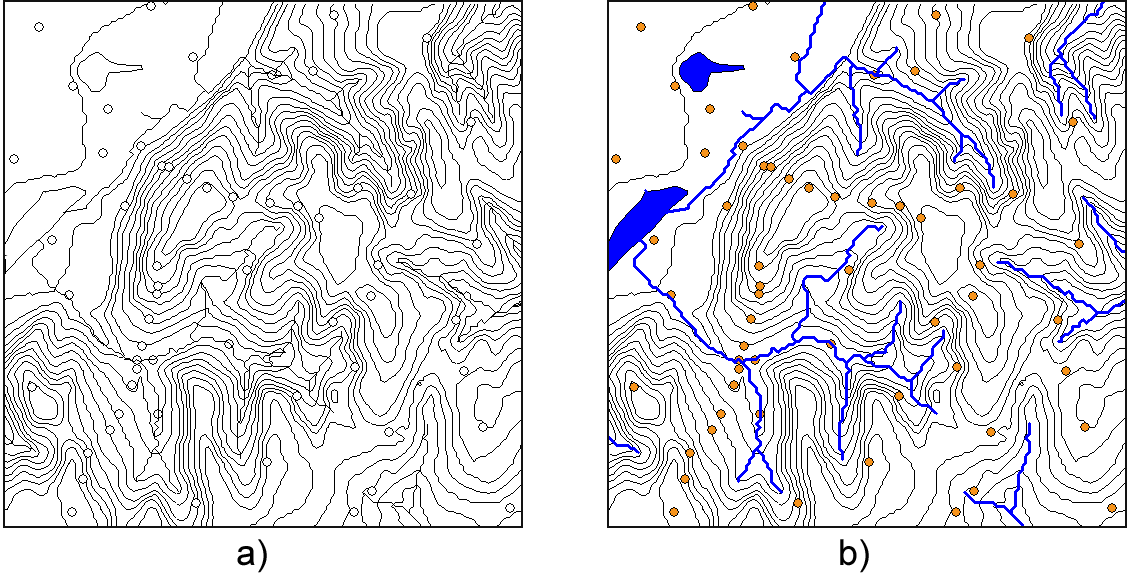
\includegraphics[width=\columnwidth]{Visualizacion/JerarquiaMapa.png}
\caption{\small Mapa con jerarqu�a incorrecta (a) y mapa adecuadamente jerarquizado (b).}
\label{Fig:JerarquiaMapa} 
\end{figure}


\section{El mapa y la comunicaci�n cartogr�fica}

El mapa es un medio de comunicaci�n visual que constituye un lenguaje con un objetivo particular: la \textbf{descripci�n de relaciones espaciales}. Un mapa es, pues, una abstracci�n simb�lica de alg�n fen�meno real, lo cual significa que presenta un cierto grado de simplificaci�n y generalizaci�n.

El lenguaje visual que ya conocemos se convierte ahora en un lenguaje cartogr�fico al adaptarlo al caso particular de la creaci�n de mapas, y sus reglas son imprescindibles para poder crear cartograf�a que facilite la labor posterior del usuario. Las conjunto de ideas relativas a la producci�n de mapas dan forma a lo que conocemos como \textbf{dise�o cartogr�fico}.

El dise�o cartogr�fico implica la toma de decisiones por parte del cart�grafo (en este caso el usuario de SIG). Estas decisiones han de estar motivadas fundamentalmente por la \textbf{utilidad del mapa} y el \textbf{p�blico al que va destinado}, y en funci�n de estas han de elegirse aspectos como la \textbf{proyecci�n} a utilizar (no necesariamente la misma en que se encuentran las capas que se van a incluir en el mapa), la \textbf{escala} (dependiendo del nivel de detalle que se desee comunicar, y siempre dentro de las limitaciones de los propios datos), el \textbf{tipo de mapa} (m�s adelante en este cap�tulo detallaremos los tipos m�s importantes), la cantidad de \textbf{simplificaci�n} que debe realizarse o los \textbf{s�mbolos} que han de emplearse para plasmar la informaci�n a transmitir.


Es importante distinguir entre dos tipos de cartograf�a: \textbf{cartograf�a base}, tambi�n denominada \emph{fundamental} o \emph{topogr�fica}, y \textbf{cartograf�a tem�tica}.

La cartograf�a base representa el tipo de mapa que originalmente era el objeto principal de la cartograf�a, cuando lo primordial era recoger con precisi�n \emph{qu�} hab�a sobre la Tierra, documentando a trav�s del documento cartogr�fico las caracter�sticas f�sicas de esta. 

La cartograf�a tem�tica se centra en la \textbf{representaci�n de un tema concreto} (una variable espacial dada), pudiendo esta ser de cualquier �ndole: f�sica, social, pol�tica, cultural, etc. Se excluyen de la lista de esos temas posibles a los puramente topogr�ficos, que constituyen el objeto de la cartograf�a base.

De otro modo, la cartograf�a topogr�fica representa \textbf{elementos f�sicos del terreno} (un accidente geogr�fico, el curso de un r�o, el perfil de una costa), mientras que la cartograf�a tem�tica se centra m�s en la \textbf{representaci�n de valores y atributos}.

La cartograf�a tem�tica se apoya en la cartograf�a base, ya que esta se incluye tambi�n en los mapas tem�ticos para facilitar la comprensi�n del comportamiento espacial de la variable representada y ubicar esta en un contexto geogr�fico dentro del propio mapa. 


\subsection{Los tipos de informaci�n y su representaci�n}

Sabemos ya que la componente tem�tica de la informaci�n geogr�fica puede ser de tipo num�rico o alfanum�rico, y que la primera se divide en los tipos nominal, ordinal, intervalos y razones.  La selecci�n de una forma de simbolizaci�n adecuada en funci�n de la naturaleza de la informaci�n es clave para lograr un mapa efectivo. En particular, debe emplearse una variable visual que presente la propiedad (nivel de organizaci�n) adecuado. 

Por ejemplo, las propiedades asociativa y selectiva solo son de inter�s para informaci�n cualitativa, mientras que el tama�o es la �nica variable visual con la propiedad cuantitativa, y por tanto la �nica adecuada para representar razones.

Las siguientes son algunas ideas b�sicas a este respecto referidas a los distintos tipos antes citados.


\begin{itemize}
	\item \textbf{Nominal}. La informaci�n de tipo nominal se representa adecuadamente utilizando la variable visual forma. Lo que representamos responde principalmente a la pregunta \emph{qu�} en lugar de a la pregunta \emph{cu�nto}, y est� m�s relacionado en cierto modo con la cartograf�a base que con la cartograf�a tem�tica. El uso de s�mbolos, para elementos puntuales o lineales es una soluci�n muy eficaz y habitual en este caso. Para el caso de representar �reas puede emplearse la variable visual color y emplear distintos tonos, o bien la textura
	
	La informaci�n alfanum�rica se trata a efectos de representaci�n del mismo modo que la de tipo nominal.
	

	\item \textbf{Ordinal}. A diferencia de la informaci�n nominal, en la informaci�n ordinal los valores definen un orden, por lo que la propiedad ordenada es necesaria para poder aplicarla a este caso.
	
	\item \textbf{Intervalos y razones}. Como en el caso anterior, pueden emplearse todas las variables visuales que presenten la propiedad ordenada. No debe olvidarse, no obstante, que la propiedad de mostrar el orden en t�rminos de cantidades o proporciones, que denomin�bamos cuantitativa, es exclusiva del tama�o, siendo este la variable visual m�s adecuada para representar correctamente este tipo de informaci�n.

	Frecuentemente, estos valores son de tipo real (no enteros), por lo que es adem�s necesario agruparlos en clases (intervalos). Esta agrupaci�n puede realizarse seg�n diversas metodolog�as, siendo las m�s habituales los intervalos iguales, los intervalos por percentiles, o los intervalos naturales, que tratan de disminuir la varianza de cada clase.

	El uso de una u otra metodolog�a puede tener un efecto muy notable en la representaci�n, como se muestra en la figura \ref{Fig:TiposIntervalosClases}.

	\begin{figure}[!hbt]
	\centering
	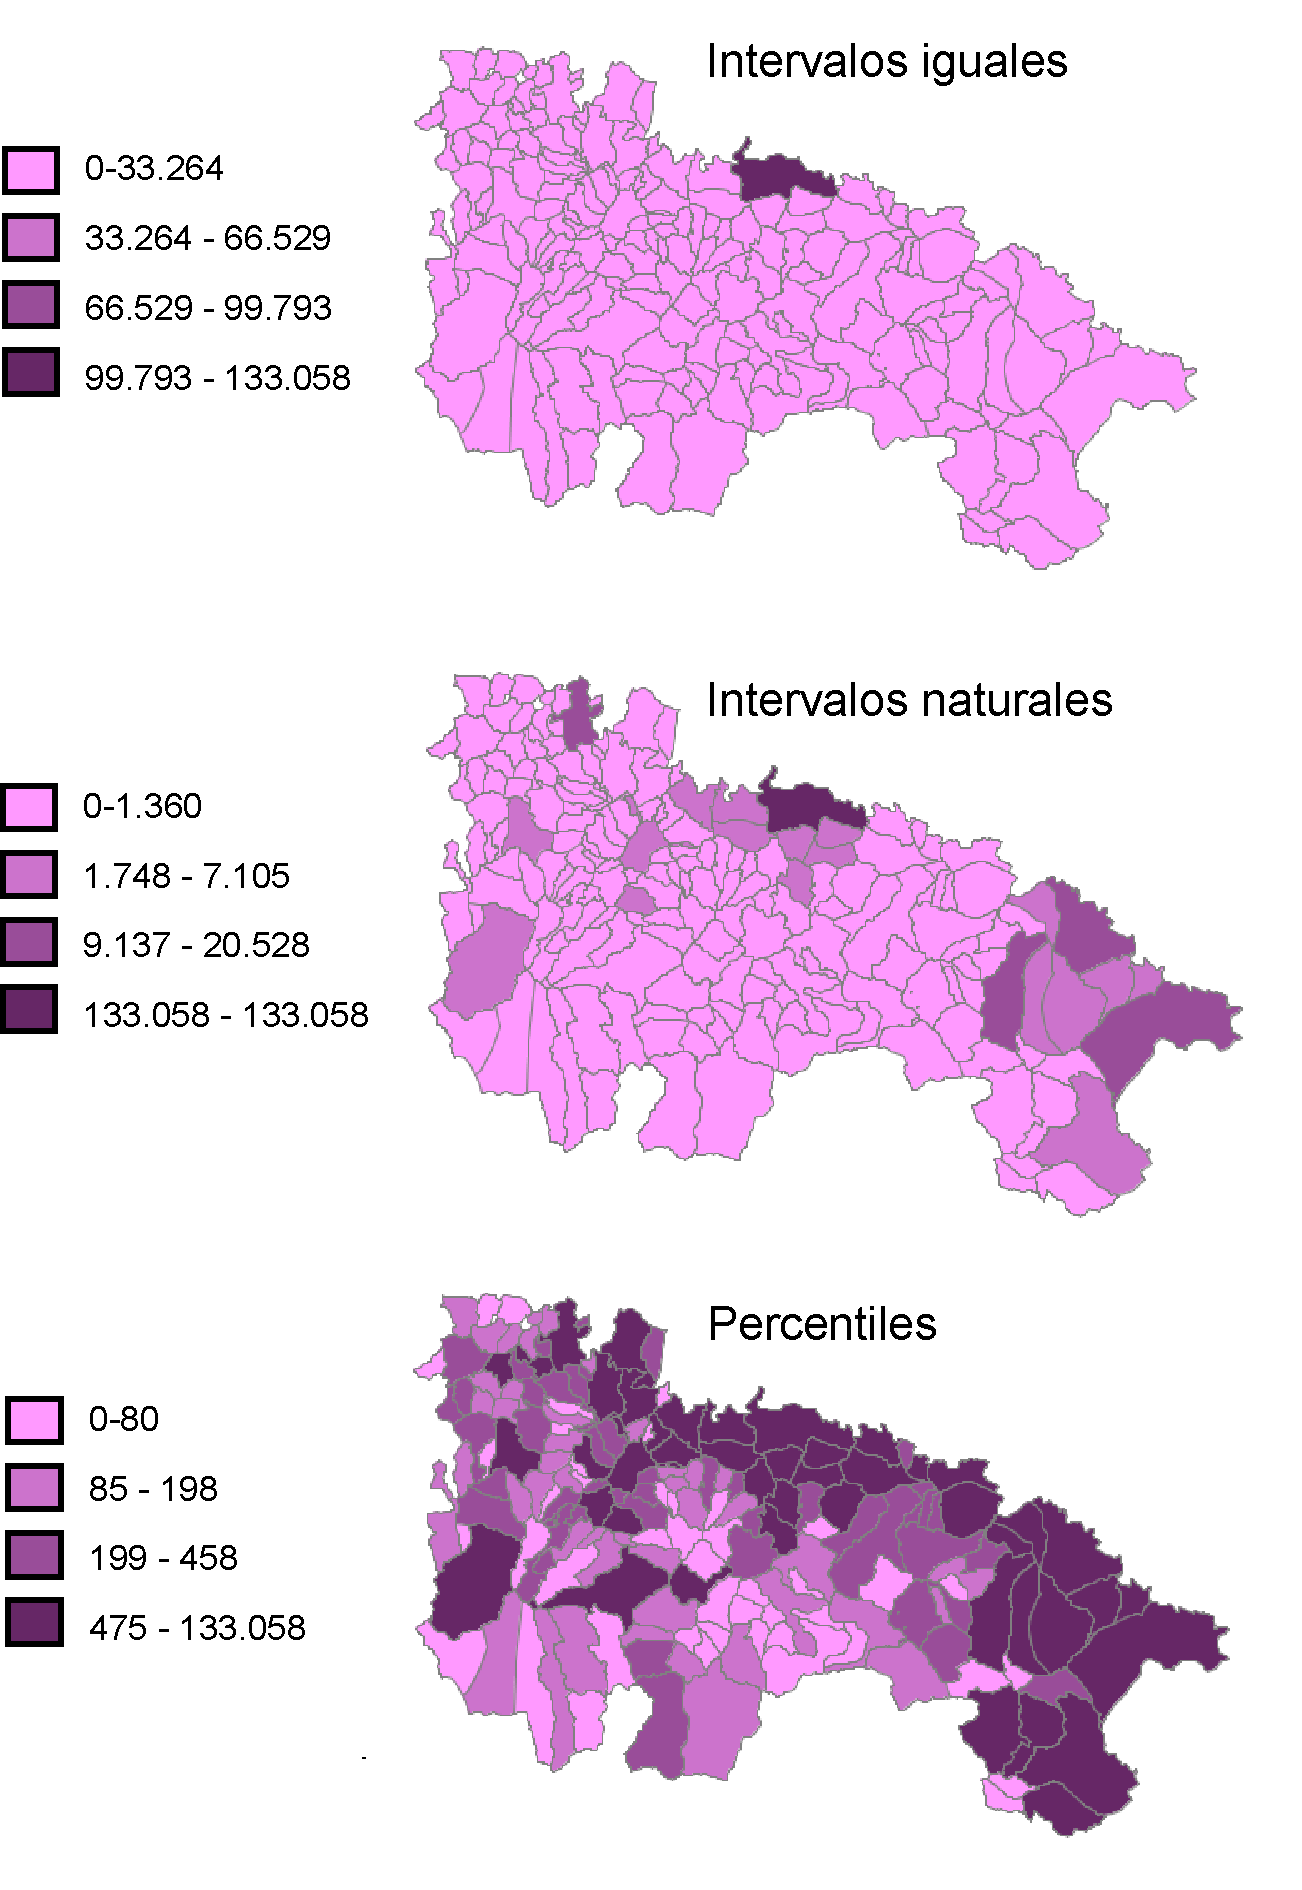
\includegraphics[width=.7\columnwidth]{Visualizacion/TiposIntervalosClases.pdf}
	\caption{\small Comparaci�n entre distintos esquemas para la creaci�n de intervalos de clase.}
	\label{Fig:TiposIntervalosClases} 
	\end{figure}


\end{itemize}


Por �ltimo, es de inter�s se�alar que, aunque los niveles de organizaci�n de las variables visuales expresan a su vez unas posibilidades crecientes (es decir, con una variable como el valor o el tama�o podemos expresar todo lo que el tono puede transmitir, ya que est�n en un nivel superior), ello no implica necesariamente que el uso de una variable de un nivel superior es mejor que otra de uno inferior. Por ejemplo, el uso del valor para un mapa con informaci�n cualitativa no es adecuado . Puesto que el valor tiene la propiedad ordenada, esto puede inducir a pensar que existe alg�n orden en la variable representada, lo cual es falso. 



\subsection{Elementos del mapa. Composici�n}

Un mapa no es solo lo que se deriva de la representaci�n de la informaci�n geogr�fica y su simbolizaci�n, sino un conjunto de elementos dispuestos de forma �ptima, siendo uno de ellos aquel que contiene la informaci�n geogr�fica como tal.

Igual de importante que simbolizar correctamente la informaci�n geogr�fica es \textbf{situar adecuadamente los distintos elementos del mapa}, ya que estos est�n pensados tambi�n, al igual que la propia simbolog�a, para facilitar la interpretaci�n de la informaci�n y hacer esta m�s comprensible.

Los siguientes son los elementos fundamentales que podemos emplear para componer un mapa (Figura \ref{Fig:ElementosMapa}):

\begin{figure}[!hbt]
\centering
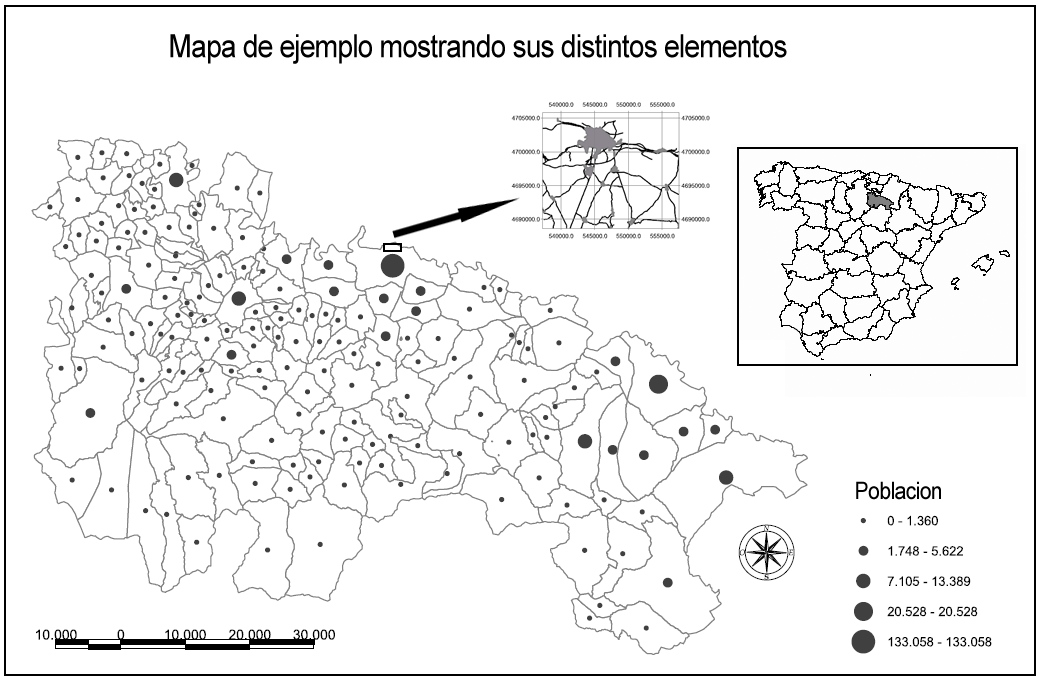
\includegraphics[width=\columnwidth]{Visualizacion/ElementosMapa.png}
\caption{\small Ejemplo de mapa mostrando sus elementos m�s habituales.}
\label{Fig:ElementosMapa} 
\end{figure}

\begin{itemize}
\item \textbf{Nombre o t�tulo}. Imprescindible para conocer qu� informaci�n muestra el mapa.
	\item \textbf{Autor}. La persona u organismo que ha creado el mapa debe aparecer indicada en alg�n punto de este.
	\item \textbf{Otra informaci�n sobre el mapa}. Por ejemplo, la relativa al sistema de referencia empleado o la fecha de su creaci�n, entre otras.
	\item \textbf{Canev�s}. El canev�s es una ret�cula que nos indica d�nde dentro de la superficie terrestre se encuentra aquello que el mapa representa, y provee la referencia geogr�fica para sus elementos. Asimismo, complementa a la escala para la estimaci�n visual de distancias y medidas. Es m�s necesario en caso de escalas bajas, aunque se a�ade con independencia de la escala.
	\item \textbf{Leyenda}. Aunque se ha de tratar de utilizar una simbolog�a lo m�s expresiva posible, no toda la informaci�n puede incorporarse en el mapa, y es necesario acompa�arlo de una leyenda. Esta ha de ser tambi�n f�cil de interpretar y lo m�s clara posible. Una leyenda demasiado extensa o de dif�cil comprensi�n probablemente nos indica que la simbolog�a escogida es mejorable.
	
	
	La leyenda y el mapa en s� forman un todo, por lo que no deben separarse mediante un cuadro, salvo en el caso en que el mapa cubra todo el �rea del lienzo y no sea f�cil separar visualmente de forma clara ambos elementos.
	\item \textbf{Norte}. Aunque habitualmente se presupone la orientaci�n Norte--Sur, no siempre ha de ocurrir as�, y una aguja apuntando al norte o una rosa de los vientos sirve para aclarar la orientaci�n del mapa. 
	\item \textbf{Escala}. La escala debe indicarse tanto de forma num�rica como gr�fica, de modo que puedan realizarse c�lculos y estimar visualmente distancias entre puntos dados del mapa.\index{Escala}
	\item \textbf{Localizador}. Un localizador provee un elemento visual para situar el mapa en un contexto geogr�fico m�s amplio. Es de especial inter�s en el caso de series de mapas, para establecer la relaci�n entre el presente y los restantes dentro de la misma serie. En este caso, el localizador sirve como mapa �ndice.
	\item \textbf{Mapas de detalle}. Cuando resulta necesario mostrar una cierta zona del mapa con mayor detalle y a una escala mayor, se puede incluir un mapa correspondiente a esa zona como un enclavado dentro del mapa principal. Se debe se�alar asimismo sobre este �ltimo la zona a la que corresponde el mapa de detalle.
\end{itemize}



Asimismo, es importante que el dise�o del mapa recalque su prop�sito, haciendo �nfasis en los aspectos m�s relevantes para cumplir este.


\section{Tipos de mapas tem�ticos}

Existen diversas alternativas en funci�n del tipo de elemento que se pretenda simbolizar o las caracter�sticas de la variable tratada, y la elecci�n de una u otra supondr� una diferencia importante en el mapa obtenido y en su uso posterior. En un mismo mapa pueden combinarse varias de estas formas, especialmente si se pretende representar m�s de una variable, en cuyo caso la combinaci�n debe buscar la m�xima claridad en la representaci�n de todas ellas.

En este apartado detallaremos los siguientes tipos de mapas tem�ticos: mapas de coropletas, mapas de isol�neas, mapas de densidad de puntos y mapas de s�mbolos proporcionales. Todos ellos se utilizan para la representaci�n de variables cuantitativas.


\subsection{Mapas de s�mbolos proporcionales}

Un mapa de s�mbolos proporcionales representa \textbf{variables cuantitativas} a trav�s de s�mbolos cuyo \textbf{tama�o est� en relaci�n con el valor} a representar de dicha variable. Es decir, emplea la \textbf{variable visual tama�o} (la �nica con la propiedad cuantitativa) para transmitir el valor de la variable representada. Si el s�mbolo es lineal, como por ejemplo una barra, el escalado de los s�mbolos para los distintos valores se realiza utilizando la longitud. Es decir, a un valor doble le corresponde una barra del doble de longitud. En el caso de s�mbolos de superficie, se emplea la superficie. Por ejemplo, en el caso de usar c�rculos, a un valor doble no le corresponde un circulo de radio doble, sino uno de �rea doble.

El escalado de s�mbolos se puede dar de forma continua, aunque resulta m�s conveniente efectuar un escalado discreto, creando clases y asignando a cada una de ellas un �nico tama�o. 

Para evitar problemas de percepci�n del tama�o, es importante mostrar en la leyenda la relaci�n entre los distintos tama�os de los s�mbolos y sus valores, como se muestra en la figura \ref{Fig:EjemplosLeyendaSimbolosProporcionales}

\begin{figure}[!hbt]
\centering
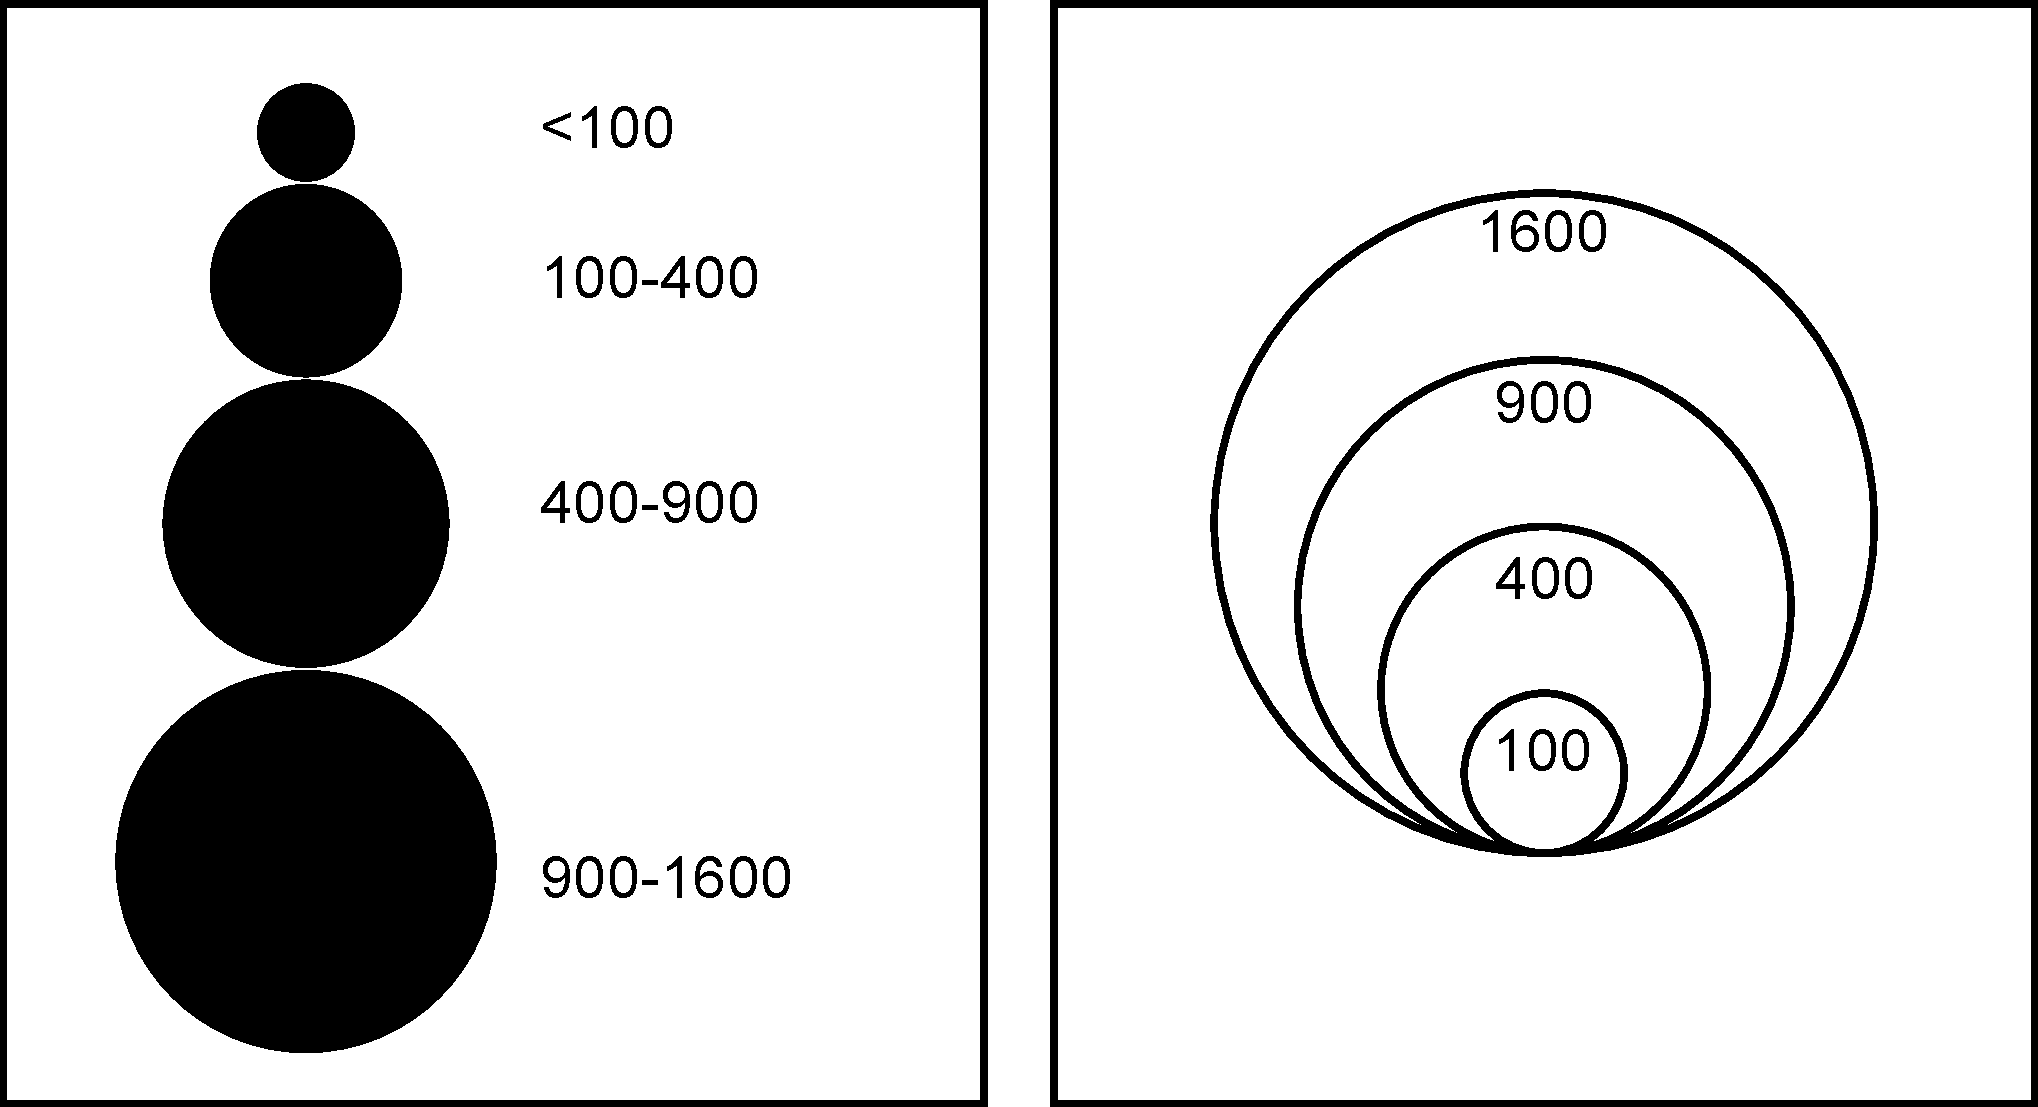
\includegraphics[width=.65\columnwidth]{Visualizacion/EjemplosLeyendaSimbolosProporcionales.pdf}
\caption{\small Dos ejemplos de leyendas para un mapa de s�mbolos proporcionales.}
\label{Fig:EjemplosLeyendaSimbolosProporcionales} 
\end{figure}


\subsection{Mapas de puntos}\index{Mapa!de puntos}

Los mapas de puntos se emplean especialmente para \textbf{variables que representan alg�n tipo de cantidad}, tales como la poblaci�n, el gasto medio por persona o la producci�n de un determinado cultivo. Estas cantidades se representan mediante la \textbf{repetici�n de puntos}, en numero proporcional a su magnitud. Cada uno de esos puntos representa un valor unitario, y el conjunto de ellos sobre la zona en cuesti�n suma la cantidad total a representar. Los puntos tienen todos la misma forma y tama�o, a diferencia de lo que vimos en el caso de los s�mbolos proporcionales. Son especialmente adecuados para variables discretas (valores enteros)

Tres son los aspectos que deben tenerse en cuenta a la hora de elaborar un mapa de puntos: el \textbf{valor de cada punto} (es decir, cu�ntas unidades de la variable representa cada punto), su \textbf{tama�o} y su \textbf{posici�n}.

El valor de cada punto se debe establecer \textbf{en funci�n de los valores m�nimo y m�ximo} de la variable, para que resulte en un mapa en el que los puntos no aparezcan en demas�a o sean demasiado escasos. Este valor se representar� en la leyenda para su interpretaci�n, habitualmente en forma de texto, escribiendo por ejemplo, que <<un punto equivale a 1000 habitantes>>.

La elecci�n del tama�o del punto debe garantizar la buena visibilidad de este, al tiempo que no debe ser excesivamente grande para que no ocupe demasiado espacio y dificulte la visi�n de otros. El \textbf{tama�o �ptimo est� en relaci�n con el valor unitario} escogido, y ambos par�metros deben establecerse conjuntamente para lograr la combinaci�n m�s adecuada.

La posici�n del punto es de gran importancia para transmitir la informaci�n correcta y no dar lugar ambig�edades o incorporar errores conceptuales. Si no disponemos de informaci�n adicional y solo tenemos el valor correspondiente a una zona dada, los puntos se han de disponer de forma regular ocupando toda la superficie de la zona. Si, por el contrario, sabemos algo m�s acerca de la distribuci�n de la variable, debemos emplear esa informaci�n para emplazarlos de forma m�s realista. Si, por ejemplo, la zona corresponde a una provincia y sabemos la localizaci�n de la principal ciudad dentro de ella, es m�s l�gico situar m�s puntos cerca del emplazamiento de esa ciudad que en otras partes de la provincia, ya que una mayor parte de la poblaci�n estar� all�.

Otro aspecto a considerar es el significado de la variable que se representa y la posibilidad o no de que aparezca en las distintas localizaciones de los puntos. Si la variable es, por ejemplo, el numero de ejemplares avistados de un determinado ave acu�tica, situar los puntos sobre zonas urbanas o de bosque no tiene sentido, ya que dan a entender que ah� hay presencia de esa especie (tantos ejemplares como los puntos en cuesti�n indiquen), algo que es falso.


La imagen \ref{Fig:MapaPuntos} muestra un ejemplo de un mapa de puntos.


\begin{figure}[!hbt]
\centering
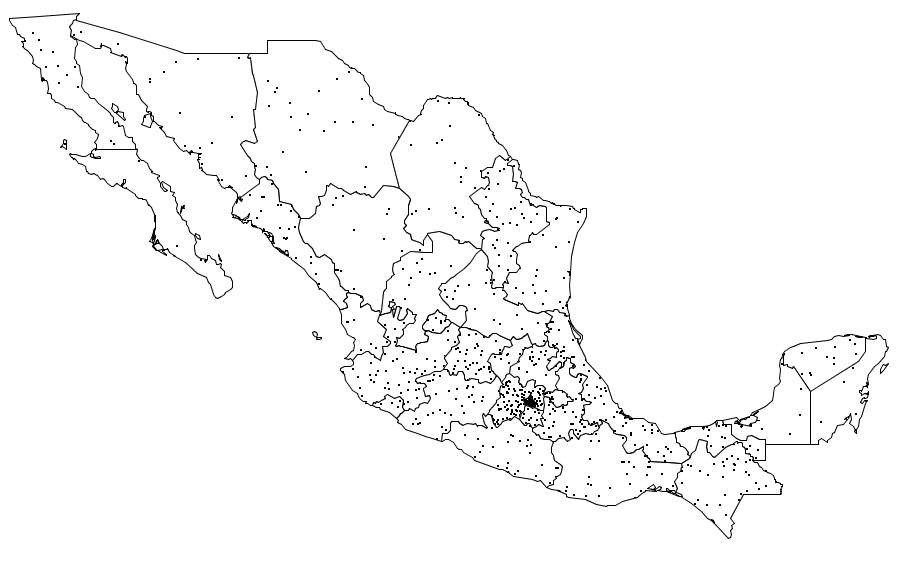
\includegraphics[width=.8\columnwidth]{Visualizacion/MapaPuntos.png}
\caption{\small Mapa de puntos.}
\label{Fig:MapaPuntos} 
\end{figure}


\subsection{Mapas de isol�neas}

Los mapas de isol�neas son muy utilizados para la representaci�n de \textbf{variables continuas}. Se combinan adecuadamente con otros tipos de mapas, ya que, al representarse �nicamente mediante l�neas, permite la presencia de otros elementos dentro del mapa sin resultar obstrusiva.

Un mapa de isol�neas est� formado por un conjunto de l�neas, cada una de las cuales une \textbf{puntos que presentan el mismo valor} de la variable. Estas l�neas no pueden cruzarse, ya que ello significar�a que en un punto se presentan dos valores. El caso m�s t�pico de mapa de isol�neas son las curvas de nivel que aparecen el un mapa topogr�fico, indicando la elevaci�n del terreno.

La representaci�n de isol�neas viene definida por la denominada \textbf{equidistancia}, que indica la diferencia entre los valores dedos isol�neas contiguas. Una menor equidistancia implica un mayor n�mero de isol�neas y una representaci�n m�s densa.

La variable visual tama�o es la �nica que suele emplearse para simbolizar isol�neas, en particular para se�alar aquellas l�neas que representan un valor m�ltiplo de una determinada cantidad y hacer as� m�s f�cil la lectura del mapa. Estas l�neas son lo que se conoce como \textbf{curvas directrices}. 

\begin{figure}[!hbt]
\centering
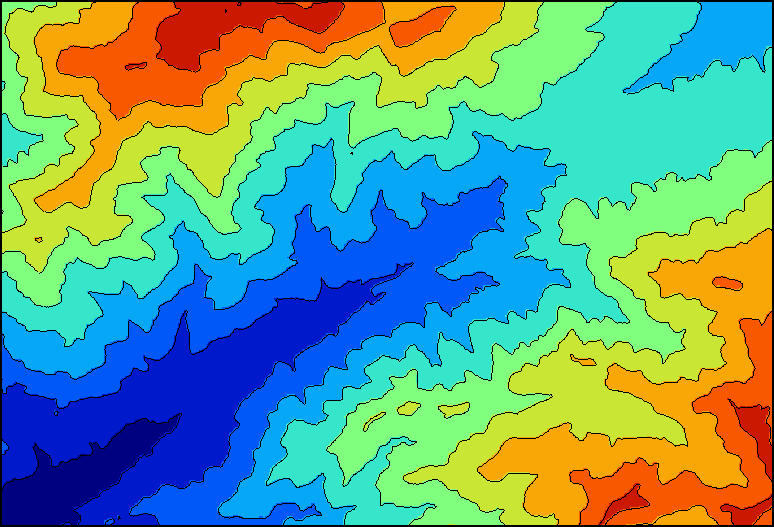
\includegraphics[width=.8\columnwidth]{Visualizacion/Isolineas.png}
\caption{\small Mapa de isol�neas. Se ha empleado para su representaci�n tanto las l�neas como el coloreado de las franjas entre estas.}
\label{Fig:Isolineas} 
\end{figure}


Las l�neas se etiquetan con el valor que representan (con texto sobre la l�nea), y se aprovecha el hecho de que dos l�neas consecutivas est�n separadas siempre por una magnitud igual a la equidistancia, lo cual aporta un importante contexto en lo que a los valores se refiere. 

Una forma particular de representar las isol�neas mediante color es hacerlo no sobre las l�neas, sino sobre las zonas que median entre ellas. Es decir, representar la clase en lugar del l�mite de clase. Este tipo de mapas se asemeja al mapa de coropletas (que veremos seguidamente), trat�ndose m�s de un mapa de �reas que de l�neas, por lo que se conoce como de \emph{isocoropletas}. Ambos tipos de representaci�n, mediante �reas y mediante l�neas, pueden combinarse en un �nico mapa.\index{Isocoropletas}

En la figura \ref{Fig:Isolineas} puede verse un ejemplo de mapa de isol�neas combinando las dos formas anteriores.


\subsection{Mapas de coropletas}\index{Mapa!de coropletas}

Los mapas de coropletas son utilizados habitualmente para representar la informaci�n geogr�fica en un SIG. Por ejemplo, los mapas de la figura \ref{Fig:TiposIntervalosClases} son todos ellos mapas de coropletas.

En un mapa de coropletas se tiene una serie de �reas definidas, cada una de las cuales posee un valor de una variable. Este valor de la variable afecta a todo el �rea y es el que se representa por medio de alguna variable visual, normalmente el color a trav�s de su componente valor.

Los mapas de coropletas adolecen de ciertos inconvenientes, siendo los principales la \textbf{sensaci�n de cambio brusco en los l�mites entre �reas}, la cual puede transmitir la idea de que en esa frontera los valores de la variable cambian bruscamente, ocultando la continuidad de la variable en caso de existir esta,, y la \textbf{homogeneidad dentro de cada �rea}, que puede no ser cierta.

Para transmitir correctamente la informaci�n, es importante normalizar la variable en funci�n de la superficie de cada unidad. Por ejemplo, en el caso de representar la poblaci�n de una serie de t�rminos municipales, es m�s adecuado representar la poblaci�n por unidad de �rea, dividiendo el valor de poblaci�n cada unidad entre la superficie de esta.


\section{La visualizaci�n en un SIG}


Una vez que conocemos los conceptos b�sicos sobre representaci�n gr�fica y su uso para la elaboraci�n de mapas, es momento de ver c�mo estos se aplican en el contexto de un SIG. Dos aspectos son especialmente relevantes a este respecto: el hecho de \textbf{contar con m�ltiples capas} que han de representarse conjuntamente, y las \textbf{particularidades de la representaci�n en pantalla}, con la interactividad que el SIG ofrece.


\subsection{Combinaci�n de capas}

En general, una capa aislada no constituye la forma �ptima de visualizar esta. Si en un mapa encontramos elementos variados, ello no obedece a la mera econom�a de espacio, sino a que a�adir informaci�n adicional a la de esa capa que queremos representar nos ayuda a entenderla mejor. Los procesos que tienen lugar en el espacio est�n relacionados unos con otros, y \textbf{visualizar esas relaciones aporta una mayor riqueza a la visualizaci�n}, haciendo que sea m�s sencillo extraer la informaci�n contenida en ella. 

Aunque sencillo de llevar a cabo en lo que a manejo del SIG respecta, combinar capas es un proceso que tambi�n debe realizarse con conocimiento y en el que, si se realiza correctamente, las diferencias pueden ser notables. No solo se trata de dar espacio dentro del mapa a toda la informaci�n que esas capas contienen, sino que exista una sinergia entre ellas en la medida de lo posible, para que se complementen mutuamente como partes de un conjunto. 


La configuraci�n fundamental en este sentido es el \textbf{orden de las capas}, que indica c�mo se disponen estas las unas sobre las otras y define el orden de pintado. Si una misma zona est� ocupada por elementos de varias capas, solo ser�n visibles los correspondientes a la capa superior, ya que la representaci�n de los pertenecientes a las dem�s quedar� oculta. 

Sabemos que las capas r�ster llenan todo el espacio y contienen valores en todas sus celdas (o p�xeles en el caso de im�genes). Por ello, van a tapar lo que se sit�e por debajo de ellas y no resulta buena idea situarlas en lo alto del orden de pintado. En su lugar, se deben considerar como \textbf{capas base sobre las que situar las restantes}, de tal modo que no impidan a estas visualizarse correctamente.

Con un razonamiento similar, podemos establecer la mejor forma de ordenar las capas vectoriales, situando por norma general los pol�gonos y encima de estos las l�neas y los puntos respectivamente. 


En ocasiones, un determinado orden viene \textbf{impuesto por el significado} que tienen las capas. Por ejemplo, si nuestro mapa contiene una capa con la red de drenaje y otra con carreteras, lo l�gico y habitual es que las carreteras est�n por encima de los r�os, ya que lo normal es que pasen por encima de estos y no al contrario. 


Una funcionalidad de que disponen los SIG para la combinaci�n de capas es el uso de \textbf{transparencias} totales o parciales. Estas se pueden aplicar tanto a capas r�ster como vectoriales, de forma que puede verse a trav�s de ellas y as� presentar la informaci�n de otras capas que se encuentren por debajo. Por ejemplo, la representaci�n mostrada en la figura \ref{Fig:CombinacionCapas} hace uso de esta t�cnica. El pol�gono que delimita la cuenca vertiente es semi--transparente, de tal modo que la capa de relieve sombreado que est� debajo puede verse, dando la sensaci�n de que sigue ese relieve.

\begin{figure}[!hbt]
\centering
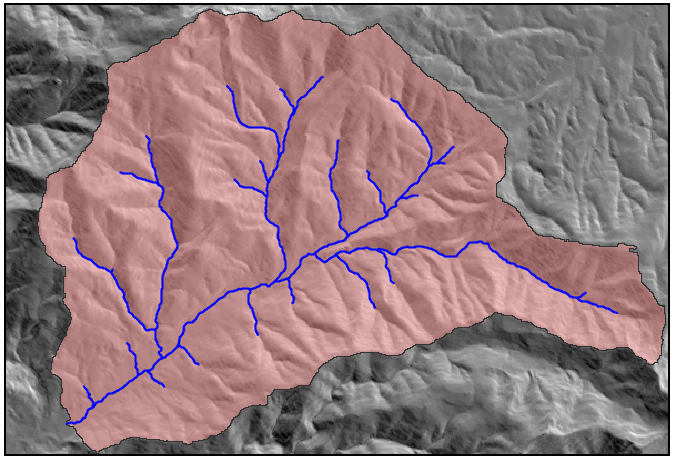
\includegraphics[width=.7\columnwidth]{Visualizacion/CombinacionCapas.png}
\caption{\small Combinaci�n de capas mediante transparencia.}
\label{Fig:CombinacionCapas} 
\end{figure}

En el caso de una capa r�ster, puede aplicarse una transparencia total, haciendo que determinadas partes de esta no se representen, en funci�n de sus valores.

En el caso en que una variable se encuentre dividida en \textbf{varias capas} (divisi�n horizontal), debe asignarse una \textbf{misma simbolog�a} a todas esas capas, con el fin de que la representaci�n sea coherente.


\subsection{Particularidades de la representaci�n en pantalla}

Tanto para las representaciones en papel como para las representaciones en pantalla se siguen unos mismos principios a la hora de dise�arlas, pero estas �ltimas presentan algunas caracter�sticas particulares que hacen necesario tener en consideraci�n otros factores. 

Podemos distinguir dos bloques fundamentales de diferencias que hacen que un mapa pensado para ser visualizado en la pantalla mientras ejecutamos un SIG no deba dise�arse exactamente igual que si estuviera pensado exclusivamente para ser utilizado en un soporte impreso: la \textbf{baja resoluci�n de la pantalla} y la \textbf{interactividad} de la propia representaci�n.


A la hora de preparar cartograf�a impresa, la resoluci�n no es un problema, ya que las capacidades de que se dispone superan a las necesidades que el cart�grafo puede tener. En la pantalla, sin embargo, algunos elementos pueden no aparecer con suficiente claridad y, aunque en papel cumplan su funci�n correctamente, es conveniente sustituirlos por otros m�s adecuados cuando no se trabaja sobre un medio impreso. Entre los elementos a evitar se encuentran las \textbf{fuentes con ornamentos} tales como sombreados, las \textbf{fuentes con serifas} (peque�os adornos al final de las l�neas para facilitar la lectura) o los \textbf{rellenos o punteados de paso muy fino}.

Respecto a la interactividad de las representaciones, debe tenerse presente que, a diferencia de un mapa impreso, en un SIG lo que vemos no es un elemento est�tico, sino din�mico. En este contexto, \emph{din�mico} no quiere decir que el mapa cambie o que represente un proceso din�mico, sino que el usuario puede alterarlo utilizando por lo menos las herramientas m�s fundamentales que proporcionan interactividad, tales como el desplazamiento, el acercamiento o el alejamiento. 

Por ejemplo, el hecho de que la escala de la representaci�n pueda variar seg�n la voluntad del usuario puede causar problemas con algunos de sus elementos  tales como s�mbolos o etiquetas de texto. Si todos los elementos del mapa se escalan proporcionalmente, una reducci�n importante de escala disminuir� el tama�o del texto hasta hacerlo ilegible. Por el contrario, si aumentamos la escala el tama�o puede ser excesivo. La figura \ref{Fig:ProblemasRepresentacionSimbolos} muestra este hecho. 


\begin{figure}[!hbt]
\centering
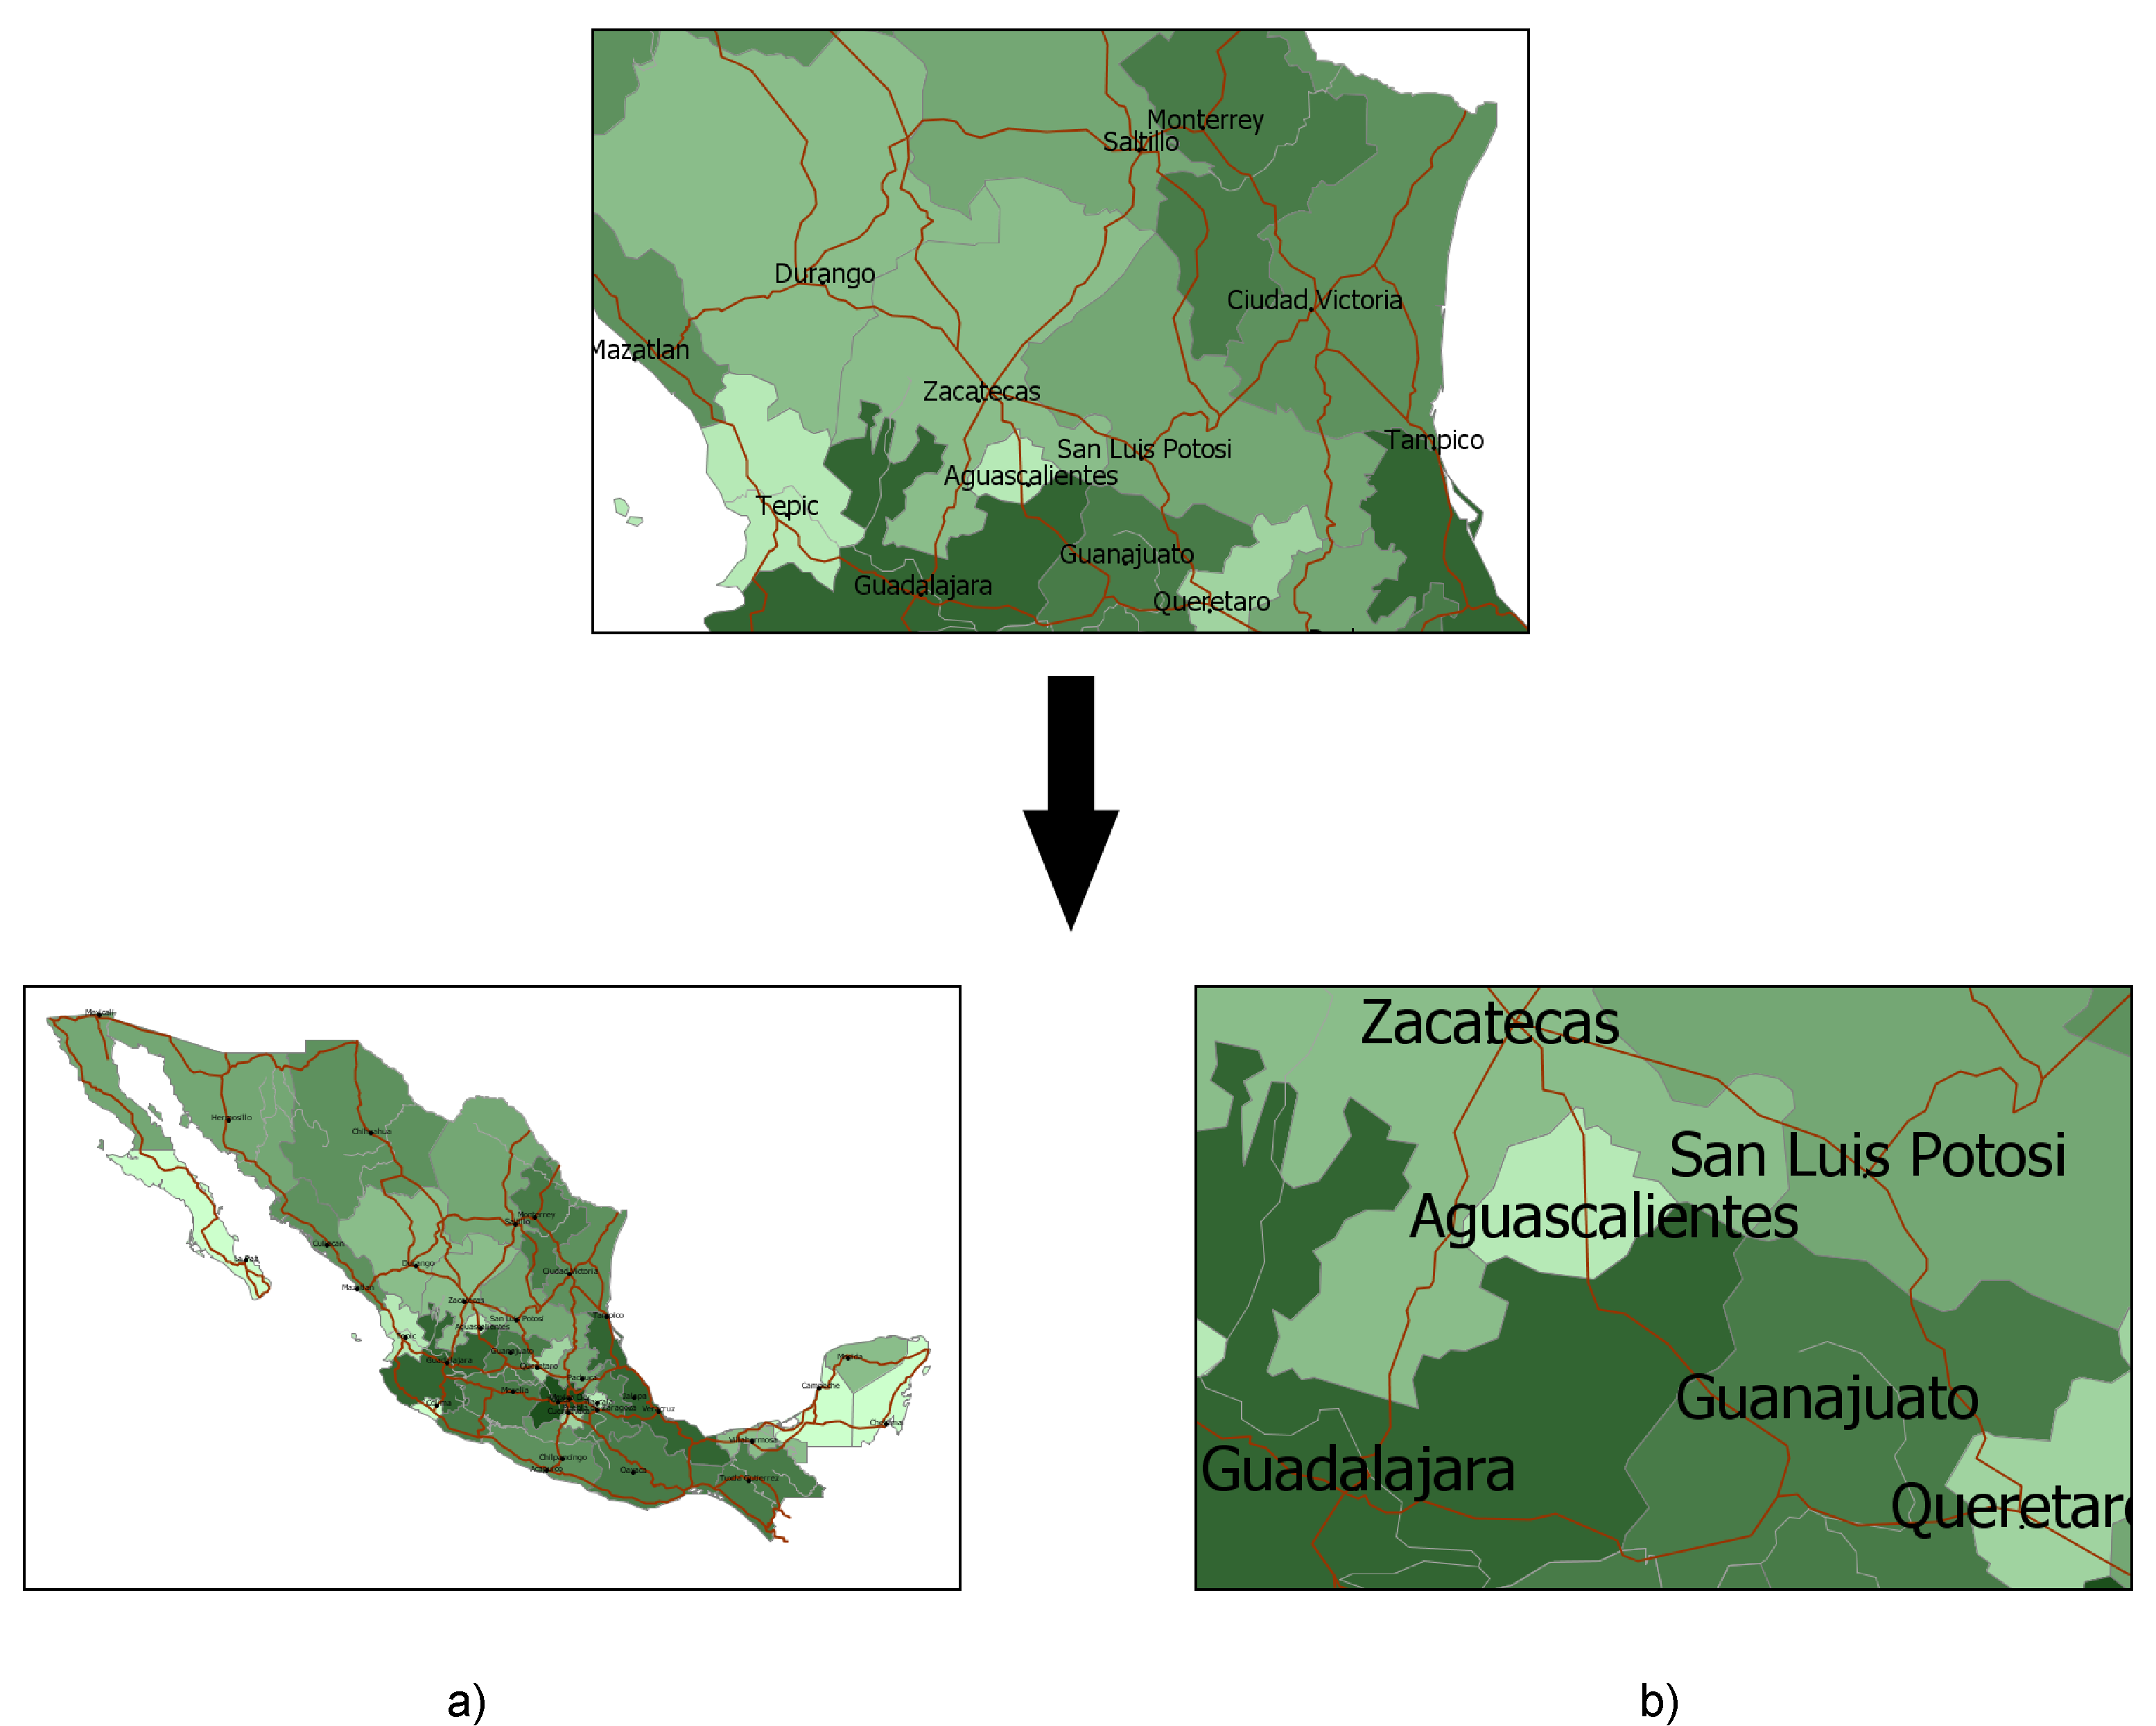
\includegraphics[width=\columnwidth]{Visualizacion/ProblemasRepresentacionSimbolos.pdf}
\caption{\small El cambio de escala var�a el tama�o de los s�mbolos tales como las etiquetas, haci�ndolos demasiado peque�os (a) o demasiado grandes (b)}
\label{Fig:ProblemasRepresentacionSimbolos} 
\end{figure}


Una soluci�n a esto es especificar un \textbf{tama�o absoluto} de estos elementos que no var�e con la escala. Es decir, que un s�mbolo o una etiqueta de texto tengan siempre el mismo tama�o en pantalla y ocupen los mismos p�xeles. A escalas bajas, sin embargo, este m�todo puede dar lugar a representaciones saturadas, como se observa en la figura \ref{Fig:RepresentacionSaturada}.

\begin{figure}[!hbt]
\centering
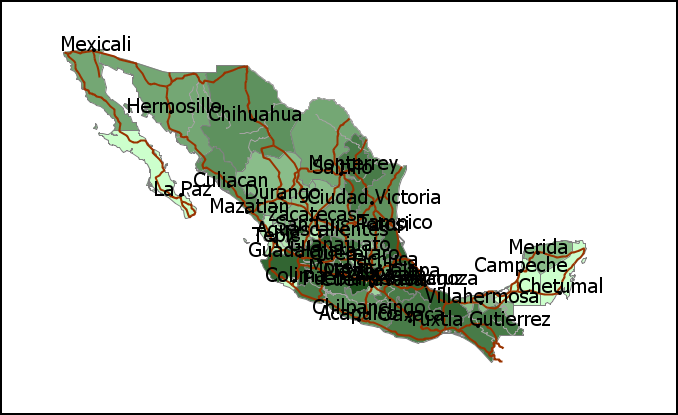
\includegraphics[width=.9\columnwidth]{Visualizacion/RepresentacionSaturada.png}
\caption{\small Representaci�n saturada al representar elementos con tama�o fijo a una escala baja.}
\label{Fig:RepresentacionSaturada} 
\end{figure}

La posibilidad de representar capas a distintas escalas, puede tambi�n dar lugar a \textbf{problemas de rendimiento}. Para evitar estos, se recomienda un \textbf{planteamiento multi--escalar} en el que, seg�n la escala, se visualicen unas u otras capas, as� como trabajar con capas de menor detalle a escalas peque�as

\pagestyle{empty} 
\tableofcontents
\end{mainmatter}

\cleardoublepage

\end{document}


